%% This is a shortened version of the notes
\documentclass[a4paper,twoside]{book}
\usepackage{geometry}
\usepackage[notheorems]{beamerarticle}
%\includeonly{privacy}
\makeindex

\mode<presentation>{
  % \useinnertheme{rectangles}
  %\useoutertheme{infolines}
  % \usecolortheme{crane}
  % \usecolortheme{rose}
}
%% Pre-amble - commonly defined macros.

%% Packages
\usepackage{fixltx2e}
\usepackage{amsmath}
\usepackage{amsfonts}
\usepackage{amssymb}
\usepackage{amsbsy}
\usepackage{isomath}
\usepackage{amsthm}
\usepackage{dsfont}
%%\usepackage{theorem}
\usepackage{algorithm}
\usepackage{algorithmicx}
\usepackage{algpseudocode}
\usepackage{mathrsfs}
\usepackage{epsfig}
\usepackage{subcaption}
\usepackage{makeidx} 
\usepackage{colortbl}
\usepackage{enumerate}
\usepackage{multirow}
\usepackage{listings}
\usepackage{pgfplots}
\usepackage{fontawesome}
\newlength\fheight
\newlength\fwidth
\only<presentation>{
\setlength\fheight{\columnheight}
\setlength\fwidth{\columnwidth}
}
\only<article>{
\setlength\fheight{0.25\textheight}
\setlength\fwidth{0.5\textwidth}
}
\usepackage[sort&compress,comma,super]{natbib}
\def\newblock{} % To avoid a compilation error about a function \newblock undefined
\usepackage{hyperref}

\setbeamertemplate{theorems}[numbered] 
\mode<presentation>{
\theoremstyle{plain}
\newtheorem{assumption}{Assumption}
\theoremstyle{definition}
\newtheorem{exercise}{Exercise}
\theoremstyle{remark}
\newtheorem{remark}{Remark}
}

\numberwithin{equation}{section} 
\mode<article>{
  \theoremstyle{plain}
  % \newtheorem{assumption}{Assumption}[section]
  \newtheorem{lemma}{Lemma}[section]
  \newtheorem{theorem}{Theorem}[section]
  \newtheorem{corollary}{Corollary}[section]
  \theoremstyle{definition}
  \newtheorem{definition}{Definition}[section]
  \theoremstyle{remark}
  \newtheorem{remark}{Remark}[section]

  % \theoremstyle{plain} \newtheorem{remark}{Remark}[section]
  % \theoremstyle{plain} \newtheorem{definition}{Definition}[section]
  \theoremstyle{plain} \newtheorem{assumption}{Assumption}[section]
  
  %%% Examples %%%%
  \newtheoremstyle{example}  % Name
  {1em}       % Space above 
  {1em}       % Space below
  {\small}      % Body font
  {}          % Indent amount 
  {\scshape}  % Theorem head font
  {.}         % Punctuation after theorem head
  {.5em}      % Space after theorem head
  {}          % Theorem head spec
  \theoremstyle{example}
  \newtheorem{example}{Example}
  \newtheorem{exercise}{Exercise}

  \usepackage{framed}
  \usepackage[framemethod=tikz]{mdframed}
  \mdfsetup{%
    roundcorner=10pt}
  \renewenvironment{block}[1]
  {\begin{mdframed}[backgroundcolor=black!10,frametitle={#1}]}
    {\end{mdframed}}

  \renewenvironment{exampleblock}[1]
  {\begin{mdframed}[backgroundcolor=blue!10,frametitle={\faGears{} #1}]}
    {\end{mdframed}}


  \renewenvironment{alertblock}[1]
  {\begin{mdframed}[backgroundcolor=green!10,frametitle={{\fontencoding{U}\fontfamily{futs}\selectfont\char 66\relax} #1}]}
    {\end{mdframed}}


  \newenvironment{theoryblock}[1]
  {\begin{mdframed}[backgroundcolor=yellow!10,frametitle={\Coffeecup #1}]}
    {\end{mdframed}}

  \newenvironment{exerciseblock}[1]
  {\begin{mdframed}[backgroundcolor=red!10,frametitle={\faPencilSquareO{} #1}]}
    {\end{mdframed}}
}
%\theoremstyle{plain} \newtheorem{conjecture}{Conjecture}[section]
%\theoremstyle{plain} \newtheorem{theorem}{Theorem}[section]
%\theoremstyle{plain} \newtheorem{proposition}{Proposition}[section]
%\theoremstyle{plain} \newtheorem{lemma}{Lemma}[section]
%\theoremstyle{plain} \newtheorem{corollary}{Corollary}[section]


%\newenvironment{proof}[1][Proof]{\begin{trivlist}
%\item[\hskip \labelsep {\bfseries #1}]}{\end{trivlist}}
%\newcommand{\qed}{\nobreak \ifvmode \relax \else
%      \ifdim\lastskip<1.5em \hskip-\lastskip
%      \hskip1.5em plus0em minus0.5em \fi \nobreak
%      \vrule height0.5em width0.5em depth0.25em\fi}

\newcommand \indexmargin[1] {\marginpar{\emph{#1}}\index{#1}}
\newcommand \marginref[2] {\marginpar{\emph{#1}}\emph{#1}\index{#2}}
\newcommand \emindex[1] {\emph{#1}\marginpar{\emph{#1}}\index{#1}}


\newcommand \E {\mathop{\mbox{\ensuremath{\mathbb{E}}}}\nolimits}
\newcommand \hE {\hat{\mathop{\mbox{\ensuremath{\mathbb{E}}}}\nolimits}}
\renewcommand \Pr {\mathop{\mbox{\ensuremath{\mathbb{P}}}}\nolimits}
\newcommand \given {\mathrel{|}}
\newcommand \gvn {|}
\newcommand \eq {{=}}


%% Special characters
\newcommand\Reals {{\mathbb{R}}}
\newcommand\Naturals {{\mathbb{N}}} 
\newcommand\Simplex {\mathbold{\Delta}}

\newcommand \FB {{\mathfrak{B}}}
\newcommand \FD {{\mathfrak{D}}}
\newcommand \FF {{\mathfrak{F}}}
\newcommand \FM {{\mathfrak{M}}}
\newcommand \FK {{\mathfrak{K}}}
\newcommand \FJ {{\mathfrak{J}}}
\newcommand \FL {{\mathfrak{L}}}
\newcommand \FO {{\mathfrak{O}}}
\newcommand \FS {{\mathfrak{S}}}
\newcommand \FT {{\mathfrak{T}}}
\newcommand \FP {{\mathfrak{P}}}
\newcommand \FR {{\mathfrak{R}}}


\newcommand \CA {{\mathcal{A}}}
\newcommand \CB {{\mathcal{B}}}
\newcommand \CC {{\mathcal{C}}}
\newcommand \CD {{\mathcal{D}}}
\newcommand \CE {{\mathcal{E}}}
\newcommand \CF {{\mathcal{F}}}
\newcommand \CG {{\mathcal{G}}}
\newcommand \CH {{\mathcal{H}}}
\newcommand \CJ {{\mathcal{J}}}
\newcommand \CL {{\mathcal{L}}}
\newcommand \CM {{\mathcal{M}}}
\newcommand \CN {{\mathcal{N}}}
\newcommand \CO {{\mathcal{O}}}
\newcommand \CP {{\mathcal{P}}}
\newcommand \CQ {{\mathcal{Q}}}
\newcommand \CR {{\mathcal{R}}}
\newcommand \CS {{\mathcal{S}}}
\newcommand \CT {{\mathcal{T}}}
\newcommand \CU {{\mathcal{U}}}
\newcommand \CV {{\mathcal{V}}}
\newcommand \CW {{\mathcal{W}}}
\newcommand \CX {{\mathcal{X}}}
\newcommand \CY {{\mathcal{Y}}}
\newcommand \CZ {{\mathcal{Z}}}

\newcommand \BA {{\mathbb{A}}}
\newcommand \BI {{\mathbb{I}}}
\newcommand \BS {{\mathbb{S}}}

\newcommand \bx {{\vectorsym{x}}}
\newcommand \by {{\vectorsym{y}}}
\newcommand \bu {{\vectorsym{u}}}
\newcommand \bw {{\vectorsym{w}}}
\newcommand \ba {{\vectorsym{a}}}
\newcommand \bc {{\vectorsym{c}}}
\newcommand \bz {{\vectorsym{z}}}
\newcommand \bq {{\vectorsym{q}}}
\newcommand \bat {{\vectorsym{a}_t}}
\newcommand \bh {{\vectorsym{h}}}
\newcommand \bo {{\vectorsym{o}}}
\newcommand \bp {{\vectorsym{p}}}
\newcommand \bs {{\vectorsym{s}}}
\newcommand \br {{\vectorsym{r}}}

\newcommand \SA {\mathscr{A}}
\newcommand \SB {\mathscr{B}}
\newcommand \SC {\mathscr{C}}
\newcommand \SF {\mathscr{F}}
\newcommand \SG {\mathscr{G}}
\newcommand \SH {\mathscr{H}}
\newcommand \SJ {\mathscr{J}}
\newcommand \SL {\mathscr{L}}
\newcommand \SP {\mathscr{P}}
\newcommand \SR {\mathscr{R}}
%%\newcommand \SS {\mathscr{S}}
\newcommand \ST {\mathscr{T}}
\newcommand \SU {\mathscr{U}}
\newcommand \SV {\mathscr{V}}
\newcommand \SW {\mathscr{W}}

\newcommand \hM {\widehat{M}}

\newcommand \KL[2] {\mathbb{D}\left( #1 \| #2 \right)}


%\newcommand \p {\partial}

\newcommand \then{\Rightarrow}
\newcommand \defn {\mathrel{\triangleq}}
%\newcommand \StateSet {{\CQ}}


%% Commands

\newcommand \argmax{\mathop{\rm arg\,max}}
\newcommand \argmin{\mathop{\rm arg\,min}}
\newcommand \dtan{\mathop{\rm dtan}}
\newcommand \sgn{\mathop{\rm sgn}}
\newcommand \trace{\mathop{\rm tr}}

\newcommand \onenorm[1]{\left\|#1\right\|_1}
\newcommand \pnorm[2]{\left\|#1\right\|_{#2}}
\newcommand \inftynorm[1]{\left\right\|#1\|_\infty}
\newcommand \norm[1]{\left\|#1\right\|}

%%\newcommand \defn {\triangleq}
%%\newcommand \defn {\equiv}
%%\newcommand \defn {\coloneq}
%%\newcommand \defn {\stackrel{\text{\tiny def}}{=}}
%%\newcommand \defn {\stackrel{\text{def}}{\hbox{\equalsfill}}}

\DeclareMathAlphabet{\mathpzc}{OT1}{pzc}{m}{it}

\newcommand \Normal {\mathop{\mathpzc{N}}\nolimits}
\newcommand \Poisson {\mathop{\mathpzc{Poisson}}\nolimits}
\newcommand \Multinomial {\mathop{\mathpzc{Multinomial}}\nolimits}
\newcommand \Dirichlet {\mathop{\mathpzc{Dirichlet}}\nolimits}
\newcommand \Student {\mathop{\mathpzc{Student}}\nolimits}
\newcommand \Bernoulli {\mathop{\mathpzc{Bernoulli}}\nolimits}
\newcommand \BetaDist   {\mathop{\mathpzc{Beta}}\nolimits}
\newcommand \Singular   {\mathop{\mathpzc{D}}\nolimits}
\newcommand \GammaDist {\mathop{\mathpzc{Gamma}}\nolimits}
\newcommand \Softmax{\mathop{\mathpzc{Softmax}}\nolimits}
\newcommand \Exp{\mathop{\mathpzc{Exp}}\nolimits}
\newcommand \Uniform{\mathop{\mathpzc{Unif}}\nolimits}
\newcommand \Laplace {\mathop{\mathpzc{Laplace}}\nolimits}

\newcommand \Param {\Theta}
\newcommand \param {\theta}
\newcommand \vparam {\vectorsym{\theta}}
\newcommand \mparam {\matrixsym{\Theta}}
\newcommand \Hyperparam {\Phi}
\newcommand \hyperparam {\phi}
\newcommand \family {\mathcal{F}}
\newcommand{\ie}{\emph{i.e.}~}
\newcommand{\eg}{\emph{e.g.}~}
\newcommand{\etal}{\emph{et al.}~}
\newcommand{\constg}{}
\newcommand{\Bel}{\mathcal{B}}
\newcommand \Bay {\ensuremath{\mathscr{B}}}
\newcommand \Adv {\ensuremath{\mathscr{A}}}

\newcommand \step {\eta}

\newcommand \Borel[1] {\FF(#1)}
\newcommand \Probs[1] {\FM(#1)}


\newcommand \pol {\pi}
\newcommand \Pol {\Pi}
\newcommand \mdp {\mu}
\newcommand \MDP {\CM}
\newcommand \meanMDP {{\bar{\mdp}_\xi}}

\newcommand {\msqr} {\vrule height0.33cm width0.44cm}
\newcommand {\bsqr} {\vrule height0.55cm width0.66cm}

\newcommand\ind[1]{\mathop{\mbox{\ensuremath{\mathbb{I}}}}\left\{#1\right\}}
\newcommand\Ind{\mbox{\bf{I}}}

\newcommand\dd{\,\mathrm{d}}

\newcommand \seq[2]{#1^{#2}}
\newcommand \pseq[3]{#1_{#2}^{#3}}
\newcommand \sam[2]{#1^{(#2)}}
\newcommand \transpose[1] {#1^\top}
\newcommand\set[1] {\left\{#1\right\}}
\newcommand\tuple[1] {\left\langle #1\right\rangle}
\newcommand\cset[2] {\left\{#1 ~\middle|~ #2\right\}}
\newcommand \ceil[1]{\left\lceil #1 \right\rceil}





\newcommand{\indep}{\mathrel{\text{\scalebox{1.07}{$\perp\mkern-10mu\perp$}}}}


\newcommand \eqlike {\eqsim}
\newcommand \gtlike {\succ}
\newcommand \ltlike {\prec}
\newcommand \gelike {\succsim}
\newcommand \lelike {\precsim}

\newcommand \eqpref {\eqsim^*}
\newcommand \gtpref {\succ^*}
\newcommand \ltpref {\prec^*}
\newcommand \gepref {\succsim^*}
\newcommand \lepref {\precsim^*}

\newcommand \util {U}
\newcommand \BUtil {U^*}
\newcommand \MUtil {\matrixsym{U}}
\newcommand \risk {\sigma}
\newcommand \Brisk {\sigma^*}
\newcommand \Loss {\ell}
\newcommand \Regret {L}
\newcommand \regret {\ell}
\newcommand \Reward {\SR}
\newcommand \reward {r}
\newcommand \vreward {\vectorsym{r}}
\newcommand \Rew {\rho}
\newcommand \boutcome {\vectorsym{\omega}}
\newcommand \outcome {\omega}
\newcommand \Outcome {\Omega}
\newcommand \act {a}
\newcommand \Act {\CA}
\newcommand \decision {a}
\newcommand \Decision {\mathcal{A}}
\newcommand \dec {\delta}
\newcommand \Dec {\mathscr{D}}


\newcommand {\MH} {\matrixsym{H}}

\newcommand \alg {\lambda}
\newcommand \Alg {\Lambda}
\newcommand \KNN {\textsc{k-NN}}

\newcommand \model {\mu}
\newcommand \MAP {\model_{\textrm{MAP}}}
\newcommand \Model {\CM}
\newcommand \Datasets {\CD}
\newcommand \Data {D}
\newcommand \Training {D_T}
\newcommand \Holdout {D_H}
\newcommand \Testing {D^*}
\newcommand \error {\epsilon}
\newcommand \obs {x}
\newcommand \Obs {\CX}
\newcommand \Att {\CA}
\newcommand \att {a}
\newcommand \attv {v}
\newcommand \Attv {\CV}
\newcommand \cls {y}
\newcommand \Cls {\CY}
\newcommand \Entropy {\mathbb{H}}
\newcommand \Gain {\mathbb{G}}


\newcommand \IDThree {\texttt{ID3}}

\newcommand \nactions {A}
\newcommand \nclasses {C}
\newcommand \nstates{S}
\newcommand \nobservations {N}
\newcommand \ndata{T}

\newcommand \figwidth {0.6\textwidth}
\newcommand \figheight {0.4\textwidth}

\newcommand \eye {\matrixsym{I}}
\newcommand \MA {\matrixsym{A}}
\newcommand \MC {\matrixsym{C}}
\newcommand \MX {\matrixsym{X}}
\newcommand \MR {\matrixsym{R}}
\newcommand \MY {\matrixsym{Y}}
\newcommand \MB {\matrixsym{B}}
\newcommand \MV {\matrixsym{V}}
\newcommand \MW {\matrixsym{W}}
\newcommand \MP {\matrixsym{P}}
\newcommand \MZ {\matrixsym{Z}}

\newcommand \vg {\vectorsym{\gamma}}
\newcommand \vp {\vectorsym{p}}
\newcommand \vs {\vectorsym{s}}
\newcommand \vx {\vectorsym{x}}
\newcommand \vr {\vectorsym{r}}
\newcommand \vm {\vectorsym{m}}
\newcommand \vb {\vectorsym{b}}
\newcommand \vt {\vectorsym{\theta}}

\newcommand \pn[1] {\vx_{[#1]}}

\newcommand \basis {f}
\newcommand \bel {\beta}
\newcommand \hyper {\omega}
\newcommand \mbel {\bel^D}
\newcommand \pbel {\bel^C}

\newcommand \pmean {\matrixsym{M}}
\newcommand \pcov {\matrixsym{C}}
\newcommand \pwish {\matrixsym{W}}
\newcommand \porder {n}

\newcommand \Syx {\matrixsym{\Sigma}_{yx}}
\newcommand \Sxx {\matrixsym{\Sigma}_{xx}}
\newcommand \Syy {\matrixsym{\Sigma}_{yy}}
\newcommand \Symx {\matrixsym{\Sigma}_{y\mid x}}

\newcommand \trans {\matrixsym{P}}
\newcommand \ident {\matrixsym{I}}

\newcommand \noise {\vectorsym{\varepsilon}}

\newcommand \pt {p_t}


\newcommand \CSet {G}
\newcommand \Parent[1] {\mathfrak{P}(#1)}
\newcommand \Children[1] {\mathfrak{C}(#1)}
\newcommand \Ancestors[1] {\mathfrak{A}(#1)}
\newcommand \Descendants[1] {\mathfrak{D}(#1)}
\newcommand \metric[2] {\nu(#1, #2)}
\newcommand \zooming {\zeta}
\newcommand \depth[1] {d(#1)}

\newcommand \sensitivity[1] {\mathbb{L}\left(#1\right)}
\newcommand \disc {\gamma}
\newcommand \Value {V}
\newcommand \val {\vectorsym{v}}
\newcommand \Vals {\mathcal{V}}
\newcommand \qval {\vectorsym{q}}
\newcommand \Qvals {\mathcal{Q}}
\newcommand \blm {\mathscr{L}}
\newcommand \tdm {\mathscr{D}}
\newcommand \pim {\mathscr{B}}



\newcommand \dist[2]{D\left(#1 ~\middle\|~ #2\right)}

\newcommand \Ae {A_\epsilon^\hist}

\newcommand \lrdist[2]{d_{lr}(#1, #2)}
\newcommand \xdistChar{\rho}
\newcommand \xdist[2]{\xdistChar(#1, #2)}
\newcommand \pdist[2]{\kappa(#1, #2)}
\newcommand{\constScale}{\omega}
\newcommand{\constScaleB}{\kappa}

\newcommand \fields[1]{\sigma(#1)}

\newcommand \hist {h}

\newcommand \abs[1] {\left|#1\right|}

\newcommand{\errorband}[5][]{ % x column, y column, error column, optional argument for setting style of the area plot
\pgfplotstableread[col sep=comma, skip first n=2]{#2}\datatable
% Lower bound (invisible plot)
\addplot [draw=none, stack plots=y, forget plot] table [
x={#3},
y expr=\thisrow{#4}-\thisrow{#5}
] {\datatable};

% Stack twice the error, draw as area plot
\addplot [draw=none, fill=gray!40, stack plots=y, area legend, #1] table [
x={#3},
y expr=2*\thisrow{#5}
] {\datatable} \closedcycle;

% Reset stack using invisible plot
\addplot [forget plot, stack plots=y,draw=none] table [x={#3}, y expr=-(\thisrow{#4}+\thisrow{#5})] {\datatable};
}


%%% macros to make things smalller
% For comparison, the existing overlap macros:
% \def\llap#1{\hbox to 0pt{\hss#1}}
% \def\rlap#1{\hbox to 0pt{#1\hss}}
\def\clap#1{\hbox to 0pt{\hss#1\hss}}
\def\mathllap{\mathpalette\mathllapinternal}
\def\mathrlap{\mathpalette\mathrlapinternal}
\def\mathclap{\mathpalette\mathclapinternal}
\def\mathllapinternal#1#2{%
\llap{$\mathsurround=0pt#1{#2}$}}
\def\mathrlapinternal#1#2{%
\rlap{$\mathsurround=0pt#1{#2}$}}
\def\mathclapinternal#1#2{%
\clap{$\mathsurround=0pt#1{#2}$}}


\usepackage{tikz}
\usepackage{tikzsymbols}
%\usetikzlibrary{external}
%\tikzexternalize[prefix=tikz/]
\usepackage{gnuplot-lua-tikz}


\usetikzlibrary{automata}
\usetikzlibrary{topaths}
\usetikzlibrary{shapes}
\usetikzlibrary{arrows}
\usetikzlibrary{decorations.markings}
\usetikzlibrary{intersections}
\usetikzlibrary{backgrounds}
\usetikzlibrary{positioning}


\tikzstyle{utility}=[diamond,draw=black,draw=blue!50,fill=blue!10,inner sep=0mm, minimum size=8mm]
\tikzstyle{select}=[rectangle,draw=black,draw=blue!50,fill=blue!10,inner sep=0mm, minimum size=6mm]
\tikzstyle{hidden}=[dashed,draw=black,fill=red!10]
\tikzstyle{RV}=[circle,draw=black,draw=blue!50,fill=blue!10,inner sep=0mm, minimum size=6mm]
\tikzstyle{place}=[circle,draw=black,draw=blue!50,fill=blue!20,inner sep=0mm, minimum size=9mm]
\tikzstyle{transition}=[rectangle,draw=black!50,fill=black!20,thick]
\tikzstyle{observed}=[circle,draw=black,draw=blue!50,fill=blue!10,inner sep=0mm, minimum size=6mm]
\tikzstyle{someset}=[circle,draw=black,minimum size=8mm]

\tikzstyle{known}=[rectangle,draw=green!50,fill=green!20,thick]
\tikzstyle{queried}=[rectangle,draw=blue!50,fill=blue!20,thick]
%\tikzstyle{transition}=[rectangle,draw=black!50,fill=black!20,thick]

\tikzstyle{thickarrow}=[->, >=latex, line width=15pt, green!50]
\tikzstyle{medarrow}=[->, >=latex,  line width=5pt]
\tikzstyle{arrow}=[->,>=triangle 60]

\tikzset{every picture/.style={
    line width=1
  }
}

\definecolor{dark-green}{rgb}{0,0.5,0}




\begin{document}



\title{Machine learning in science and society}
\subtitle{From automated science to beneficial artificial intelligence}
\author[C. Dimitrakakis]{Christos Dimitrakakis}


\maketitle

\chapter*{Preface}

This book is a technical introduction to important aspects of machine learning in science and society. It covers the most fundamental concepts in privacy, fairness, causality, reproducibility and experiment design. While I have tried to make the book as rigorous as possible, in the interest of brevity some technical details are omitted. 

However, even though the book is not addressed to a technical audience, every concept is necessarily connected to precise technical definition. This includes the bare minimum amount of theoretical development for a thorough understanding of the main concepts. Throughout the book, we use Bayesian decision theory and graphical models to offer a unifying perspective on those issues.


Throughout the book, we will use the following blocks of text for particular types of material.
\begin{exampleblock}{An example.}
Such blocks contain illustrations and examples. 
\end{exampleblock}

\begin{alertblock}{An important note.}
Important caveats or properties of algorithms will be given in such blocks.
\end{alertblock}

\begin{theoryblock}{Theoretical note.}
Discussions of a more theoretical nature, or notes that require some additional thinking.
\end{theoryblock}

\begin{exerciseblock}{Exercise.}
  These exercises are meant to be done individually, either while reading the text, or in class.
\end{exerciseblock}

\begin{groupactivity}{Group activity.}
  These activities are meant to be done in class.
\end{groupactivity}

The first chapter offers an introduction to the field of machine learning in general and to fairness, privacy and reproducibility in particular. Chapter~\ref{ch:privacy} discusses privacy. Chapter~\ref{ch:fairness} talks about fairness.

I whole-heartedly recommend the book ``The Ethical Algorithm'' as a non-technical companion to this book and ``The foundations of differential privacy'' as a more thorough overview of differential privacy.



\tableofcontents


\chapter{Introduction}
\label{ch:introduction}

\only<article>{
  What this this book about?
}
\section{Introduction to machine learning}
\only<presentation>{
  \begin{frame}
    \tableofcontents[ 
    currentsection, 
    hideothersubsections, 
    sectionstyle=show/shaded
    ] 
  \end{frame}
}


\only<article>{
  % What are the central problems in machine learning?
  Problems in machine learning are similar to problems in science.
  Scientists must plan experiments intelligently and collect data.
  The must be able to use the data to verify a different hypothesis.
  More generally, they must be able to make decisions under
  uncertainty (Without uncertainty, there would be no need to gather more data).
  Similar problems appear in more mundane tasks, like learning to drive a car.
}
\only<presentation>{
  \begin{frame}
    \frametitle{Scientific applications}
    \centering
    \begin{columns}
      \begin{column}{0.5\textwidth}
        \centering
        \includegraphics[width=0.8\columnwidth]{../figures/climate.jpg}\\
        \includegraphics[width=\columnwidth]{../figures/networks-2.jpg}
      \end{column}
      \begin{column}{0.5\textwidth}
        \includegraphics[width=\columnwidth]{../figures/dark_matter.jpg}
        \\
        \includegraphics[width=\columnwidth]{../figures/protein.jpg}
      \end{column}
    \end{columns}
    \only<2>{
      \begin{tikzpicture}[remember picture,overlay]
        \draw[fill=black,opacity=0.75] 
        (current page.north east) rectangle (current page.south west);
        \node at (current page.center) {
          {\Huge \alert{Interpretability, Reproducibility}}
        };
      \end{tikzpicture}}
  \end{frame}
}

\only<article>{
  For that reason, science is a very natural application area for
  machine learning.  We can model the effects of climate change and
  how to mitigate it; discover structure in social networks; map
  the existence of dark matter in the universe by intelligently
  shifting through weak gravitational lens data, and not only study
  the mechanisms of protein folding, but discover methods to
  synthesize new drugs.

  We must be careful, however. In many cases we need to be able to
  interpret what our model tells us. We also must make sure that
  the any results we obtain are reproducible.
}

\only<presentation>{
  \begin{frame}
    \frametitle{Pervasive ``intelligent'' systems}
    \begin{columns}
      \begin{column}{0.3\textwidth}
        \centering
        \includegraphics[width=\textwidth]{../figures/echo-home.jpg}
        \\
        Home assistants

        \vspace{\fill}

        \bigskip

        \includegraphics[width=\textwidth]{../figures/tesla.jpg}
        \\
        Autonomous vehicles
      \end{column}
      \begin{column}{0.3\textwidth}
        \centering 
        \includegraphics[width=\textwidth]{../figures/web-ads.png}
        \\
        Web advertising

        \vspace{\fill}

        \bigskip

        \includegraphics[width=\textwidth]{../figures/uber-here-maps.jpg}
        \\
        Ridesharing
      \end{column}
      \begin{column}{0.3\textwidth}
        \centering 
        \\
        \includegraphics[width=\textwidth,clip = true, trim=0 0 0 42.5cm]{../figures/lending.pdf}
        \\
        Lending

        \vspace{\fill}

        \bigskip

        \includegraphics[width=\textwidth]{../figures/algorithms-public.jpg}
        \\
        Public policy
      \end{column}
    \end{columns}
    \only<2>{
      \begin{tikzpicture}[remember picture,overlay]
        \draw[fill=black,opacity=0.75] 
        (current page.north east) rectangle (current page.south west);
        \node at (current page.center) {
          {\Huge \alert{Privacy, Fairness, Safety}}
        };
      \end{tikzpicture}}
  \end{frame}
}

\only<article>{
  While machine learning models in science are typically carefully
  handcrafted by scientists and experts in machine learning and
  statistics, this is not typically the case in everyday
  applications. Nevertheless, well-known or home-grown machine
  learning models are being deployed across the application
  spectrum. This involve home assistants that try and get you want,
  web advertising, which tries to find new things for you to want,
  lending, which tries to optimally lend you money so that you buy
  what you didn't need before. We also have autonomous vehicles,
  which take you were you want to go, and ridesharing services,
  which do the same thing, but use humans instead. Finally, there
  are many applications in public policy, such as crime prevention,
  justice, and disease control which use machine learning.  In all
  those cases, we have to worry about a great many things that are
  outside the scope of the machine learning problems itself. These
  are (a) privacy: you don't want your data used in ways that you have
  not consented to (b) fairness: you don't want minorities to be
  disadvantaged and (c) safety: you don't want your car to crash.
}

\subsection{Data analysis,  learning and planning}

\only<article>{
  To make the above more concrete, let's have a look at a number of problems in machine learning. These involve learning from and analysing data, including inferring decision rules, and constructing complex plans using the evidence gleaned from the data. Machine learning problems are commonly separated in three different types: supervised, unsupervised and reinforcement learning. Typical supervised learning problems include classification and regression, while unsupervised problems include compression, clustering and topic modelling. Reinforcement learning, on the other hand, is concerned with artificially intelligent agents more generally, with examples including game playing and adaptive control. Their main differences are two. Firstly, the \emph{type} of feedback we have about learning performance. Secondly, and perhaps more importantly, whether or not the problem involves \emph{active data collection}. In this course, we will try and take a global view of these problems in the context of decision theory.
}

\only<presentation>{
  \begin{frame}
    \centering
    \Huge{What can machine learning do?}
  \end{frame}
}
\begin{frame}
  \frametitle{Can machines learn from data?}
  \begin{center}
    \only<1>{\includegraphics[width=0.8\textwidth]{../figures/text-cloud}
      \\

      {\large An unsupervised learning problem: topic modelling}
    }
    \only<2>{\includegraphics[width=0.8\textwidth]{../figures/Face-Recognition}
      \\

      {\large A supervised learning problem: object recognition}
    }
  \end{center}
\end{frame}


\only<article>{
  You can use machine learning just to analyse, or find structure in
  the data. This is generally called unsupervised learning. One such
  example is topic modelling, where you let the algorithm find topics
  from a corpus of text.  These days machines are used to learn from
  in many applications.  These include speech recognition, facial
  authentication, weather prediction, etc. In general, in these
  problems we are given a \emph{labelled} dataset with, say, example
  images from each class. Unfortunately this does not scale very
  well, because obtaining labels is expensive.

  This is partially how science works, because what we need to do
  is to find a general rule of nature from data. Starting from some
  hypothesis and some data, we reach a conclusion. However, many
  times we may need to actively experiment to obtain more data,
  perhaps because we found that our model is wrong.
}



\begin{frame}
  \frametitle{Can machines learn from their mistakes?}
  \begin{center}
    \includegraphics[width=0.7\textwidth]{../figures/rl_interaction}
  \end{center}
  \only<presentation>{
    \begin{block}{Reinforcement learning}
      Take actions $a_1, \ldots, a_t$, so as to maximise utility
      $U = \sum_{t=1}^T r_t$
    \end{block}
  }
\end{frame}


\only<article>{
  So, what happens when we make a mistake? Can we somehow recognise
  it? Humans and other animals can actually learn from their
  mistakes. Consider the proverbial rat in the maze. At some
  intervals, the experimenter places some cheese in there, and the
  rat must do a series of actions to obtain it, such as navigating
  the maze and pulling some levers. It doesn't know how to get to
  the cheese easily, but it slowly learns the layout of the maze
  through observation, and in the end, through trial-and-error it
  is able to get to the cheese very efficiently.

  We can formalise this as a reinforcement learning problem, where
  the rat takes a series of actions; at each step it also obtains a
  reward, let's say equal to 0 when it has no cheese, and 1 when it
  eats cheese. Then we can declare that the rat's utility is the sum
  of all rewards over time, i.e. the total amount of cheese it can
  eat before it dies. The rat needs to explore the environment in order to be able to
  get to the cheese. 

  An example in robotics is trying to teach a
  robot to flip pancakes. One easy thing we can try is to show the robot
  how to do it, and then let it just copy the demonstrated
  movement. However, this doesn't work! The robot needs to explore
  variations of the movement, until it manages to successfully flip
  pancakes. Again, we can formulate this as a reinforcement learning
  problem, with a reward that is high whenever the pancake's position is
  flipped, and on the pan; and low everywhere else. Then the robot can
  learn to perform this behaviour through trial and error. It's
  important to note that in this example, merely demonstration is not
  enough. Neither is reinforcement learning enough. The same thing is
  true for the recent success of AlphaGo in beating a master human:
  apart from planning, they used both demonstration data and self-play,
  so that it could learn through trial and error.  }

\begin{frame}
  \frametitle{Can machines make complex plans?}
  \begin{center}
    \includegraphics[width=0.8\textwidth]{../figures/619px-FloorGoban}
  \end{center}
\end{frame}


\only<article>{
  I suppose the first question is whether machines can plan
  ahead. Indeed, even for large problems, such as Go, machines can
  now perform at least as well as top-rated humans. How is this
  achieved?
}

\begin{frame}
  \frametitle{Machines can make complex plans!}
  \begin{center}
    \includegraphics[width=0.8\textwidth]{../figures/Tic-tac-toe-game-tree}
  \end{center}
\end{frame}


\only<article>{
  The basic construction is the planning tree. This is an enumeration
  of all possible future events. If a complete enumeration is
  impossible, a partial tree is constructed. However this requires
  evaluating non-terminal game positions. In the old times, this was
  done with heuristics, but now this is data-driven, both through the
  use of expert databases, and through self-play and reinforcement
  learning.
}


\subsection{Experiment design}

\only<presentation>{
  \begin{frame}
    \centering
    \Huge{The scientific process as machine learning}
  \end{frame}
  \begin{frame}
    \centering
    \includegraphics[width=\textwidth]{../figures/Las_Vegas_slot_machines}
  \end{frame}
}


\only<article>{
  An example that typifies trial and error learning are bandit
  problems. Imagine that you are in a Casino and you wish to
  maximise the amount of money you make during the night. There are
  a lot of machines to play. If you knew which one was the best,
  then you'd just play it all night long. However, you must also
  spend time trying out different machines, in order to get an
  estimate of how much money each one gives out. The trade off
  between trying out different machines and playing the one you
  currently think is best is called the exploration-exploitation
  trade-off and it appears in many problems of experiment design for
  science.
}


\only<presentation>{
  \begin{frame}
    \frametitle{Adam, the robot scientist}
    \centering
    \includegraphics[width=\fwidth]{../figures/robot-scientist}
  \end{frame}
}

\only<article>{
  Let's say we want to build a robot scientist and tell it to
  discover a cure for cancer. What does the scientist do and how can the robot replicate it??
}


\only<presentation>{
\begin{frame}
  \frametitle{Drug discovery}
  \centering
  \includegraphics[width=\columnwidth]{../figures/drug-discovery-000}
\end{frame}
}

\only<article>{
  Simplifying the problem a bit, consider that you have a large
  number of drug candidates for cancer and you wish to discover
  those that are active against it. The ideas is that you select
  some of them, then screen them, to sort them into active and
  inactive. However, there are too many drugs to screen, so the
  process is interactive. At each cycle, we select some drugs to
  screen, classify them, and then use this information to select
  more drugs to screen. This cycle, consequently has two parts:
  1. Selecting some drugs given our current knowledge.
  2. Updating our knowledge given new evidence.
}


\begin{frame}
  \frametitle{Drawing conclusions from results}
  \begin{figure}[H]
    \centering
    \begin{tikzpicture}[line width=2pt]
      \node at (0,0) (bt) {hypothesis}; \node[select] at (0,2) (at)
      {experiment}; \node[utility] at (3,-2) (rt) {result};
      \draw[blue,->] (at) -- (rt); \node at (4,0) (bt2) {conclusion};
      \draw[red,->] (at) -- (bt2); \draw[red,->] (bt) -- (bt2);
      \draw[red,->] (rt) -- (bt2);
    \end{tikzpicture}
    \only<article>{
      \caption{Dependence diagram between selection of an experiment, formulation of a hypothesis, and drawing of a conclusion. The result depends only on the experiment. However, the conclusion depends on the experiment, hypothesis and the obtained result. The red lines indicate computational dependencies, while the blue lines indicate physical dependencies.}
    }
    \label{fig:drawing-conclusions}
  \end{figure}
\end{frame}

\only<article>{
  In general, we would like to have some method which can draw
  conclusions from results. This involves starting with a
  hypothesis, performing an experiment to verify or refute it,
  obtain some experimental result; and then concluding for or
  against the hypothesis. Here the arrows show dependencies
  between these variables. So what do we mean by "hypothesis" in this case?
}

\subsection{Bayesian inference.}
\only<presentation>{
\begin{frame}
  \frametitle{Tycho Brahe's minute eye measurements}
  \begin{figure}[h]
    \centering
    \begin{columns}
      \begin{column}{0.45\textwidth}
        \includegraphics[width=0.9\fwidth]{../figures/circular-orbits}
      \end{column}
      \hspace{1em}
      \begin{column}{0.45\textwidth}
        \includegraphics[width=0.9\fwidth]{../figures/tycho-observations}
      \end{column}
    \end{columns}

    \caption{Tycho's measurements of the orbit of Mars and the conclusion about the actual orbits, under the assumption of an earth-centric universe with circular orbits.}
    \label{fig:tycho}
  \end{figure}
  \begin{itemize}
  \item Hypothesis: Earth-centric, Circular orbits
  \item Conclusion: \alert{Specific} circular orbits
  \end{itemize}
\end{frame}
}

\only<article>{
  Let's take the example of planetary orbits. Here Tycho famously
  spent 20 years experimentally measuring the location of Mars. He
  had a hypothesis: that planetary orbits were circular, but he
  didn't know which were the right orbits. When he tried to fit his data to this hypothesis, he concluded a specific circular orbit for Mars \ldots around Earth.
}

\only<presentation>{
  \begin{frame}
  \frametitle{Johannes Kepler's alternative hypothesis}
  \begin{columns}
    \centering
    \begin{column}{0.5\textwidth}
      \includegraphics[width=\fwidth]{../figures/orbits}
    \end{column}
    \begin{column}{0.5\textwidth}
      \includegraphics[width=\fwidth]{../figures/tycho-observations}
    \end{column}
  \end{columns}
    \begin{itemize}
    \item Hypothesis: Circular \alert{or} elliptic orbits
    \item Conclusion: Specific \alert{elliptic} orbits
    \end{itemize}
\end{frame}
}

\only<article>{
  \centering
  \begin{figure}[h]
    \begin{subfigure}{0.3\textwidth}
      \includegraphics[width=0.5\fwidth]{../figures/tycho-observations}
      \caption{Tycho's Measurements}
    \end{subfigure}
    \begin{subfigure}{0.3\textwidth}
      \includegraphics[width=0.5\fwidth]{../figures/circular-orbits}
      \caption{Tycho's conclusion}
    \end{subfigure}
    \begin{subfigure}{0.3\textwidth}
      \includegraphics[width=0.5\fwidth]{../figures/orbits}
      \caption{Kepler's conclusion}
    \end{subfigure}
    \caption{How given the same data, one can reach different conclusion depending on one's modelling assumptions.}
  \end{figure}
}

\only<article>{
  Kepler had a more general hypothesis: that orbits could be
  circular or elliptic, and he actually accepted that the planets
  orbited the sun. This led him to the broadly correct model of all
  planets being in elliptical orbits around the sun. However, the
  actual verification that all things do not revolve around earth,
  requires different experiments.
}


\only<presentation>{
  \begin{frame}
    \frametitle{200 years later, Gauss formalised this statistically}
    \begin{columns}
      \begin{column}{0.5\textwidth}
        \includegraphics[width=\fwidth]{../figures/gauss-diagram}
      \end{column}
      \begin{column}{0.5\textwidth}
        \includegraphics[width=\fwidth]{../figures/SeptemberTable}
      \end{column}
    \end{columns}
  \end{frame}
}

\only<article>{
  Later on, Gauss collected even more experimental data to calculate the orbit of Ceres. He did this using one of the first formal statistical methods; this allowed him to avoid cheating (like Kepler did, to accentuate his finding that orbits were elliptical).
}

\only<presentation>{
  \begin{frame}
    \frametitle{A warning: The dead salmon mirage}
    \includegraphics[width=\textwidth]{../figures/fmri-salmon}
  \end{frame}
}


\only<article>{
  It is quite easy to draw the wrong conclusions from applying
  machine learning / statistics to your data. For example, it was
  fashionable to perform fMRI studies in humans to see whether some
  neurons have a particular functional role. There were even
  articles saying that "we found the neurons encoding for Angelina
  Jolie". So some scientists tried to replicate those results. They
  took a dead salmon, and put it an fMRI scanner. They checked its
  brain activity when it was shown images of happy or sad
  people. Perhaps surprisingly, they found an area of the brain that
  was correlated with the pictures - so it seemed, as though the
  dead salmon could distinguish photos of happy people from sad
  ones. However, this was all due to a misapplication of
  statistics. In this course, we will try and teach you to avoid
  such mistakes.

}

\begin{frame}
  \frametitle{A simple simulation study}
  \only<article>{Sometimes we want to use a simple simulation study to understand how well our methods work. The following code is an example of how to do this. Here we are doing a simplified fMRI analysis, but the general idea is not significhey, antly different from what people actually do in the field.}
  \url{src/reproducibility/mri_analysis.ipynb}
\end{frame}

\begin{frame}
  \frametitle{Planning future experiments}
  \only<article>{
    So far we have focused only on the problem of data analysis. However, we also need to think about the problem of planning for experiments. This is called \alert{experiment design}. Experiment designs are usually fixed. In that case, we can use assumptions about the data and how much accuracy we need to design the experiment. However, it is also possible to have an adaptive experiment design where our future experiments depend on our current conclusions.
  }
  \begin{figure}
    \centering
    \begin{tikzpicture}[line width=2pt]
      \node at (0,0) (bt) {hypothesis};
      \node[select] at (0,2) (at) {experiment};
      \node[utility] at (3,-2) (rt) {result};
      \draw[blue,->] (at) -- (rt);
      \node at (4,0) (bt2) {conclusion};
      \draw[red,->] (at) -- (bt2);
      \draw[red,->] (bt) -- (bt2);
      \draw[red,->] (rt) -- (bt2);
    \end{tikzpicture}
  \end{figure}
\end{frame}

\only<article>{
  In general, optimal experiment design is indeed difficult, especially in setting such as drug discovery where the number of experiments is huge.  However, conceptually, there is a simple and elegant solution to this problem.
}


\begin{frame}
  \frametitle{Planning experiments is like Tic-Tac-Toe}
  \begin{center}
    \includegraphics[width=\textwidth]{../figures/Tic-tac-toe-game-tree}
  \end{center}
\end{frame}


\only<article>{
  The basic idea is to think of experiment design as a game between the scientist and Nature. At every step, the scientist plays an X to  denote an experiment. Then Nature responds with an Observation. The main difference from a game is that Nature is (probably) not adversarial. We can also generalise this idea to problems in robotics, etc.
}

\only<presentation>{
  \begin{frame}
    \frametitle{Eve, another robot scientist}
    \includegraphics[width=\textwidth]{../figures/eve.jpg}
    Discovered a malaria drug
  \end{frame}
}
\only<article>{
  These kinds of techniques, coming from the reinforcement learning literature have been successfully used at the university of Manchester to create a robot, called Eve, that recently (re)-discovered a malaria drug.
}

\subsection{Book overview}

\begin{frame}
  \frametitle{Machine learning in practice}
  \begin{block}{Avoiding pitfalls}
    \begin{itemize}
    \item Choosing hypotheses.
    \item Correctly interpreting conclusions.
    \item Using a good testing methodology.
    \end{itemize}
  \end{block}
  \begin{block}{Machine learning in society}
    \begin{itemize}
    \item<alert@2> Privacy \uncover<2->{--- Credit risk.}
    \item<alert@3> Fairness \uncover<3->{--- Job market.}
    \item<alert@4> Safety \uncover<4->{--- Medicine.}
    \end{itemize}
  \end{block}
\end{frame}

\only<article>{
  One of the things we want to do in this course is teach you to
  avoid common pitfalls.

  Now I want to get into a different track. So far everything has
  been about pure research, but now machine learning is pervasive:
  Our phones, cars, watches, bathrooms, kettles are connected to the
  internet and send a continuous stream of data to companies. In
  addition, many companies and government actors use machine
  learning algorithms to make or support decisions. This creates a
  number of problems in privacy, fairness and safety.
}


\begin{frame}
  \frametitle{The view from statistics}
  \only<article>{While in machine learning people generally discuss mainly supervised, unsupervised or reinforcement learning, these are actually three rather broad, but still limited categories of problems. There are many other problems, such as semi-supervised learning, active learning, imitation/apprenticeship learning, inverse reinforcement learning, preference elicitation, adaptive control, and possibly many others to come. The statistical view is that there basically three types of problems:}

  \begin{block}{Inference}\index{inference|textbf}
    Given what we know, what can we say about how the world works, the current state of the world or events in the past?
  \end{block}
  \begin{block}{Prediction.}\index{prediction|textbf}
    Can we predict specific evens in the future? \only<article>{This frequently is done through some type of inference.}
  \end{block}
  \begin{block}{Decision making.}\index{prediction|textbf}
    Given what we know, and what we want to achieve, what is the best decision we can make? \only<article>{This typically requires some ability to predict the effect of our actions.}
  \end{block}
  \only<article>{We will encounter many specific inference, prediction and decision making tasks during this course.}
\end{frame}

\begin{frame}
  \frametitle{Course structure}
  \begin{block}{Module structure}
    \begin{itemize}
    \item \alert{Activity}-based, hands-on.
    \item Mini-lectures with short exercises in each class.
    \item Technical tutorials and labs in alternate week.
    \end{itemize}
  \end{block}
  
  \begin{block}{Modules}
    Three mini-projects.
    \begin{itemize}
    \item Simple decision problems: Credit risk.
    \item Sequential problems: Medical diagnostics and treatment.
    \end{itemize}
  \end{block}
\end{frame}

\begin{frame}
  \frametitle{Technical topics}
  The book covers a number of technical topics. Sections marked with an asterisk (*) may be skipped safely upon a first reading without compromising understanding of the remaining material.
  \begin{block}{Machine learning problems}
    \begin{itemize}
    \item Unsupervised learning. \only<article>{Loosely speaking, this is simply the problem of estimating some structure from data. In statistical terms, it is usually the problem of estimating some joint distribution of random variables under some model assumptions. Problems in unsupervised learning include clustering, anomaly detection, compression}.
    \item Supervised learning. \only<article>{In this setting data can be split in two groups of variables. One group that is always available, and another group that must be predicted. A special case of the problem is when we wish to estimate some function $f : \CX \to \CY$ from data. Classical problems in this setting are classification and regression.}
    \item Reinforcement learning. \only<article>{This is a very general sequential decision problem, where an agent must learn how to behave optimally in an unknown environment only by limited feedback and reinforcement. The standard setting involves the agent trying to maximise its (expected) cumulative reward over time.}
    \end{itemize}
  \end{block}

  \begin{block}{Algorithms and models}
    \begin{itemize}
    \item Bayesian inference and graphical models.
    \item Stochastic optimisation and neural networks.
    \item Backwards induction and Markov decision processes.
    \end{itemize}
  \end{block}
\end{frame}


\begin{frame}
  \begin{block}{Further reading}
    \begin{itemize}
    \item \citet{bennett2012journal} describe how the usual
      uncorrected analysis of fMRI data leads to the conclusion that
      the dead salmon can reason about human images.
    \item \citet{Bennett2009ThePC} discuss how to perform analyses of medical images in a principled way. They also introduce the use of simulations in order to test how well a particular method is going to perform.
    \end{itemize}
  \end{block}

  \begin{block}{Resources}
    \begin{itemize}
    \item Online QA platform: \url{https://piazza.com/class/jufgabrw4d57nh}
    \item Course code and notes:  \url{https://github.com/olethrosdc/ml-society-science}
    \item Book \url{https://github.com/olethrosdc/ml-society-science/notes.pdf}
    \end{itemize}
  \end{block}
\end{frame}





%%% Local Variables: 
%%% mode: latex
%%% TeX-master: "notes.tex"
%%% End: 

\chapter{Privacy}
\label{ch:privacy}

\only<article>{ One interpretation of privacy is simply the ability to
  maintain a personal secret. Is it possible to maintain perfect
  secrecy? Can the thoughts in our head be perfectly safe, or can they
  be revealed indirectly through our actions?

  While we certainly \emph{can} securely store and transmit data using
  cryptography, the problems we will discuss in this chapter are
  \emph{not} solvable solely through cryptography. We are interested
  in scenarios where we must make a public decision or release some
  summary statistics that depend on private data, in such a way as to
  minimise harm to the individuals contributing their data.

  If we never have to reveal any of our computations, cryptography is
  what is needed. For example, through homomorphic computation, an
  untrusted party can even perform some computations on encrypted
  data, returning an encrypted result to us, while learning nothing
  about the original secret.  As long as the data, and the results of
  any computation on it, are kept under lock and key, our personal
  information cannot be revealed.

  However, sometimes we must make public decisions or release
  public information based on this data. Then it can be revealed
  indirectly. For example, you can trust your doctor to maintain
  confidentiality, but when you go to the pharmacy to get the prescribed
  medicine, somebody can infer the medical condition you suffer from.

  It is even possible to learn personal information from aggregate
  statistics.  Let us say your doctor publishes a list of cases of
  different diseases every week, together with some other information
  such as the approximate patient age. Even though your own data is
  mixed with that of all other patients, it is possible to infer your
  diagnosis, especially with some additional side-information: If
  somebody knows you were the only person in that age group visiting
  the doctor that week, they will learn your diagnosis.
  
  From that point of view, it is not the data itself, but the complete
  process of data collection, treatment and public release that can be
  characterised as private or non-private.  For that reason, we will
  emphasise an \emph{algorithmic} view of privacy: participants
  entrusts their data to an algorithm, which produces a useful output
  in return. The algorithmic process is typically not fully automated,
  as it also depends on some human input: One example is a medical
  study examining different treatments for a disease. While humans
  select and administer the treatments, they will typically rely on a
  randomised strategy for assigning treatments to individuals, and use
  a statistical method to report their results.  Given this mixture of
  ad-hoc decisions and formal algorithmic methods, is it possible to
  guarantee privacy in any sense? What kind of guarantees can we make?

  Generally speaking, an algorithm has good privacy properties, if the
  amount of information that can be revealed through the algorithm's
  output about any individual contributing data is bounded. In
  particular, we are interested in how much an adversary can learn
  about any individual's input to the algorithm from the algorithm's
  output.

  This does not preclude learning general facts about individuals from
  the output. For example, a study about the use of steroids in sports
  may show that 90\% of sprinters with times under 10 seconds are
  using steroids, while only 50\% of slower sprinters do so. Any
  sprinter with a time under 10 seconds is thus suspected of using
  steroids by association. However, it does not matter if their data
  has been used in the study. The publication of the result does not
  impact their privacy, but the amount of harm it does to them does
  not depend in their participation: the same statistical result would
  have been obtained with or without them.
  
  In this chapter, we will look at two formal concepts of privacy
  protection: $k$-anonymity and \emph{differential privacy}. The first
  is a simple method for anonymising databases. However, it provides
  only limited resistance to identification. The latter is a more
  general concept, which provides full information-theoretic
  protection to individuals. A major problem with any privacy
  definition and method, however is correct interpretation of the
  privacy concept used, and correct implementation of the algorithm
  used.
}



\section{Things we do with data}

\only<presentation>{
  \begin{frame}
    \begin{block}{Reasons for data collection}
      \begin{itemize}
      \item To publish it.
      \item To publish specific statistics.
      \item To make decisions through arbitrary computations.
      \end{itemize}
    \end{block}
  \end{frame}
} \only<article>{ How do we use data in the first place? Sometimes we
  simply publish the data, perhaps after some initial
  processing. Publication of datasets is useful for researchers that
  want to do perform further analysis on the data. Usually though, we collect data in order to calculate specific statistics. For example the census collects data about the number of people in different households, wages, etc, and then publishes tables detailing the average age and number of people per household in different areas of the country. This demographic information is useful for policy makers, urban planning to organise voting centers and the distribution of police and fire stations, as well as other public services. }


\begin{frame}
  \begin{figure}
    \centering
    \includegraphics[height=\fheight]{../figures/smbc-the-problem}
    % Copyright: SMBC comics
  \end{figure}
\end{frame}
\begin{frame}

  \only<article>{ Fundamentally, privacy in statistics is an \emph{issue of
      trust.} The analyst, be it a human, or an automated service, will
    use your data to make decisions. You must also decide who to trust
    and how much. Do we trust the data analyst? How much privacy are
    we willing to sacrifice to the analyst? How much to the public at
    large?  What you want out of the service.  Is the service
    important enough to sacrifice significant amounts of privacy? What
    is an acceptable trade-off between utility and privacy?  These are
    difficult questions and are hard to quantify, hence we assume that
    we have already decided how to answer them, and we simply want to
    find an appropriate methodology for achieving a good result.  }
  
  \only<presentation>{
    \begin{block}{An issue of trust}
      \begin{itemize}
      \item Who to trust and how much.
      \item What you want out of the service.
      \end{itemize}
    \end{block}
  }

  \only<article>{ Consider a researcher wishing to collect data for a  statistical analysis. If the analysis is eventually
    published,\footnote{If somebody knows that the analysis is being
      conducted, however, they could still learn something private from the fact that the analysis has \emph{not} been published.} this
    creates two possible scenarios for that may lead to privacy violations.}
  \begin{itemize}
  \item Publication of ``anonymised'' data.
    \only<article>{Sometimes we may collect data in order to publish the dataset itself for other researchers to use. This is common practice in machine learning, with image classification datasets being a good example. However, there is always some privacy risk even if identifying information such as names are removed.}
  \item Public data analysis. \only<article>{In this setting, we only publish summary statistics or models about the data. A prime example is a national census analysis, which may provide detailed demographic information for all towns and regions in a nation. Although only aggregate data is published, it is theoretically possible to infer personal information. For that reason, the US Census Bureau conducted its analysis in 2020 using differential private algorithms.}
  \end{itemize}
  \begin{alertblock}{Cryptography is not enough.}
    \only<presentation>{
      Cryptography provides:
      \begin{itemize}
      \item Secure communication and computation.
      \item Authentication and verification.
      \end{itemize}
      Public outputs are by definition \alert{not} protected.
    }
    \only<article>{Cryptography provides secure communication and computation, authentication and verification. These are used to establish secure channels with somebody that we trust. However, the privacy violations we are concerned with relate to \alert{publicly released} outputs of algorithms. It is not important whether or not all the data and computation are encrypted: as long as the algorithm generates a public output, it is theoretically possible for somebody to learn something about the algorithm's input.}
  \end{alertblock}


\end{frame}



\section{Statistical disclosure}

\only<presentation>{
  \begin{frame}
    \tableofcontents[ 
    currentsection, 
    hideothersubsections, 
    sectionstyle=show/shaded
    ] 
  \end{frame}
}

\only<article>{
  \begin{centering}
    \emph{``Data is everywhere'', said the statistician, ``data, data!''.}
  \end{centering}

  In the past, statistical analysis was performed
  with laboriously collected and annotated datasets. Even as
  recently as in the early 21st century, databases for machine
  learning were limited to a few thousand entries at most. At the
  time of writing, not only has the size of datasets become
  extremely large, but the sources of data are much more
  diverse. Data are collected and commercialised whenever we visit a
  website and even as we walk around with our phone. To a limited
  extent, there is a tradeoff between what we can get out of a
  service and what we pay into it. Many free services such as
  navigation software rely on collecting user data to perform
  better: If you can tell that there is a traffic jam in Central
  Avenue, you can after all try and take another route.  As long as
  informed consent exists, use of private data is generally regarded
  as unproblematic.\footnote{This is actually underscored by the
    GDPR legislation, which focuses on consent and data use
    methods.}

  However, even apparently benign data collected with appropriate
  consent can lead to serious and unexpected privacy
  violations. There are three famous examples of this: Firstly, the
  identification of people in supposedly anonymous health data in
  the 1990s in the state of Massachussets, which we will go over in
  detail in this chapter. Secondly, the identifications of users
  through anonymised movie ratings in the Netflix dataset. Finally,
  the ability to discover if any given individual's data is
  contained in a pooled genomic study.
}
\begin{frame}
  \frametitle{Anonymisation}
  \only<article>{Data is collected for many reasons. Any typical service you might want to use will require a minimal amount of data. For example, a dating service will at a minimum require your age and location, as shown in the example below.}
  \begin{example}[Typical relational database in a dating website.]
    \begin{table}[H]
      \centering
      \begin{tabular}{l|l|l|l|l|l|l}
        Birthday & Name & Height  & Weight & Age & Postcode & Profession\\
        \hline
        06/07 & \only<1>{Li Pu} & 190 & 80 & 60-70 & 1001 & Politician\\
        06/14 & \only<1>{Sara Lee} & 185 & 110 & 70+ & 1001 & Rentier\\
        01/01 & \only<1>{A. B. Student} & 170 & 70 & 40-60 & 6732 & Time Traveller
      \end{tabular} 
    \end{table}
    \only<article>{ If somebody is a user in a dating website, you
      expect them to give some minimal personal information to be
      stored in the site's database. This might include their
      birthday, location and profession, for example.} 
  \end{example}
  \only<article>{When you submit your data to a service, you expect it to be used responsibly. For the dating service, you expect it to use the information to find good matches, based on your preferences and location. Whenever somebody uses the service, they obtain some information about you, at least indirectly. For example, if they make a query for similar singles in their neighbourhood, and they see your profile, then they have learned that you live nearby.

    If we wish to publish a database, frequently we need to protect the identities of the people involved. A simple idea is to erase directly identifying information. However, this does not really work most of the time, especially since attackers can have side-information that can reveal the identities of individuals in the original data, when combined with the published dataset.
  }
  
  \only<2>{The simple act of hiding or using random identifiers is called anonymisation.}
  \only<article>{However this is generally insufficient as other identifying information may be used to re-identify individuals in the data.   In particular, even if somebody is unable to infer the information of any individual from the published, anonymised, dataset, they may be able to do so via some side-information. All that is needed is another dataset with some columns in common with the dataset they want to target.}
\end{frame}


\begin{frame}
  \frametitle{Record linkage}
  \begin{figure}
    \begin{subfigure}{0.65\textwidth}
      \centering \def\firstcircle{(0,0) circle (7em)}
      \def\secondcircle{(3,0) circle (7em)}
      
      \begin{tikzpicture}
        \uncover<1,3>{ \draw \firstcircle node[text width=7em]
          {Ethnicity\newline Date\newline Diagnosis \newline Procedure
            \newline Medication \newline Charge }; } \uncover<3>{
          \begin{scope}
            \clip \firstcircle; \fill[red] \secondcircle;
          \end{scope}
        } \uncover<2,3>{\draw \secondcircle node [text width=2em,
          align=right] {Name \newline Address \newline Registration
            \newline Party \newline Lastvote}; } \node [text width=4em]
        (QI) at (1.5, 0) {Postcode \newline Birthdate \newline Sex};
        \uncover<3>{ \node [text width=16em] (qi-text) at (1.5, -3)
          {87\% of Americans identifiable}; \path[->]<1-> (qi-text) edge [bend left]
          (QI); }
      \end{tikzpicture}
      \caption{Voter registration}
    \end{subfigure}
    \begin{subfigure}{0.3\textwidth}
      \centering
      \includegraphics[height=0.8\fheight]{../figures/Bill_Weld}
      %% Copyright: CC BY 2.0 
      \caption{Bill Weld}
    \end{subfigure}

    \caption{Linkage attack on a anonymised patient information database. A misguided attempt to release medical information as public data (left circle in figure (a)) by then-governor Bill Weld resulted in a simple linkage attack. This was done by accessing a party registration database (right circle in figure (b)) which contained three common fields with the medical database. }
  \end{figure}
  \only<article>{
    As an example, in the 1990s a the governor of Massachussets,
    decided to publish anonymised information about the health records
    of individual state employs. They were careful to hide all
    obviously identifying information such as their name, and thus
    claimed that there are no potential privacy violations. However,
    they left in some information that they thought would be useful
    for researchers: the postcode, the birthdate, and the sex of each
    individual.
    
    This allowed a PhD student, McSweeney, to perform the following
    linkage attack. She order a floppy disk containing database of
    voting records in the state. This contained names and addresses,
    as well as the postcode, birth date and sex of every voter. In that
    way, she was able to cross-reference this data, and so obtain the
    identities of individuals in that database. The first record she
    obtained was that of the governor himself, Bill Weld. Later, she
    estimated that approximately 87\% of Americans are uniquely
    identifiable through those three attributes.
  }
\end{frame}


% \begin{frame}
%   \frametitle{Data linkage with SQL}
%   The original database \verb|database| and adversary side information \verb|side-information| can be combined using the following simple SQL query:
% \begin{verbatim}
% SELECT * FROM database JOIN side-information ON [condition]
% \end{verbatim}
%   where \verb|condition| describes how to match the records.

%   \begin{example}
%     For the databases given above, we could use
% \begin{verbatim}
% SELECT * FROM tinder JOIN tax ON tinder.height = tax.height AND tinder.age = tax.age
% \end{verbatim}
%     to create a joint table.
%   \end{example}
% \end{frame}

\only<article>{ Clearly, anonymisation is not enough. So, is there a
  way to formally guarantee privacy? In the next section we will go
  over the solution of McSweeny, which provides us with an algorithmic
  definition of anonymity. While this provides some degree of
  protection against certain linkage attacks, it is sadly insufficient
  to protect privacy in general. Later, we will introduce the notion
  of differential privacy, which protects individuals against
  statistical disclosure in an information-theoretic manner.  }


\section{Algorithmic privacy.}
\only<article>{ The above discussion should help emphasise that
  \emph{a dataset} cannot be characterised as
  private or non-private. We should actually start from the
  observation that \emph{any data contributed by an individual} should
  be considered private, because it could be combined with other
  datasets to obtain sensitive personal information.

  For that reason, we wish to ensure that, whenever individuals
  contribute data for processing, the result of the processing cannot
  be used to reveal whatever information they had contributed. Thus,
  the idea of privacy only applies on \emph{algorithms} that are used
  on personal data. Generally speaking, we wish for algorithms to both
  be useful and have good privacy properties. Unfortunately, as we
  shall see in the sequel, there is a distinct trade-off between
  privacy and utility. However, let us specify more precisely what we
  mean by an algorithm.
}
\begin{frame}  
  \frametitle{What is an algorithm?}

  \only<article>{Any functional process is an algorithm. The
    information given to an algorithm for processing is called an
    \emph{input} to the algorithm. The result of the process is called
    the algorithm's \emph{output}.  In this book, identify inputs with
    observations or features $\CX$, and outputs with actions $\CA$ by
    the algorithm: i.e. we view the algorithm as taking actions that
    have an observable effect on its external environment.  Algorithms
    are usually deterministic: given the same input, they produce the
    same output. However, it is also useful to consider
    \emph{stochastic} algorithms, whose output randomly changes, even
    when the input is the same.
    
  }
  
  \begin{definition}[Stochastic algorithm $\pi$]
    A stochastic algorithm $\pi$ with input domain $\CX$ and output
    domain $\CA$ is a mapping $\pi : \CX \to \Simplex(\CA)$ from
    observations $\CX$ to \emph{distributions} over outputs
    $\Simplex(\CA$). When $\CA$ is finite, we will write
    $\pol(a \mid x)$ to denote the conditional probability that the
    algorithm outputs $a$ given input $x$.
  \end{definition}
  \only<article>{

    So, one way of seeing a stochastic algorithm is as a
    \emph{collection} of probability distributions $\pol(a \mid x)$
    over $\CA$, one for each value of $x$. This is exactly equivalent
    to the definition of a deterministic algorithm $f : \CX \to \CA$,
    which would be a simple function. This would define one specific
    value in $\CA$ (instead of a distribution) for each value of $x$.

    The above definition is fine when the output domain $\CA$ is
    finite. Then outputs $a \in \CA$ cannot have infinitesimally small
    probabilities. However, in many problems $\CA$ is a Euclidean
    subset, e.g. the interval $[0,1]$. In that case, we have two
    choices: either treat $\pol$ as a probability density, or as a
    probability measure. The latter is more general, and applies no
    matter what $\CA$ is. Formally, we can write this as follows.
    
    \begin{theoryblock}{The general case.}
      It is best to think of $\pol(\cdot | x)$ as a different probability
      measure over $\CA$ for every possible value of $x$. Then we write
      \[
        \pol(A \mid x) \defn \Pr_\pol(a \in A \mid x), \qquad A \subset \CA,
      \]
      for the conditional probability that algorithm's output is in
      some set $A \subset \CA$ given input $x$. This allows us to treat
      the case when $\CA$ is continuous or discrete with the same notation.
    \end{theoryblock}

    How can we actually obtain a stochastic algorithm? The usual
    method is to define an algorithm as usual, but with a source of
    randomness as part of its inputs, fancifully called \emph{random
      coins}. By using those random coins as part of the calculations,
    we obtain a random result, even if every step of the algorithm is
    deerministic.

    \begin{exampleblock}{Algorithmic randomness.}
      We can construct a random algorithm through access to a random
      coin $\omega$ taking values in $\Omega$. We can then define the
      output through a deterministic function $a_\pi(\omega, x)$. Since
      $\omega$ is random, the output of the function is also random.
      If $P$ is the probability distribution of $\omega$, then:
      \[
        \pi(A \mid x) = P(\cset{\omega \in \Omega}{a_\pi(\omega, x) \in A}),
      \]
      i.e. the probability that the algorithm's output is in $A$ is
      equal to the measure of the values of $\omega$ for which the
      $a_\pi(\omega, x) \in A$.
    \end{exampleblock}
  }
\end{frame}

\begin{frame}
  \frametitle{What is private?}

  \only<article>{
  The overall framework we will use in this book is that everything
  pertaining to an individual is by definition private. While in
  reality there might be some attributes that individuals might want
  to remain secret and some which are not considered important, it is
  generally impossible to predict potential harm from the disclosure
  of any individual information.  Thus, this chapter takes an
  expansive view of privacy: any information about an individual,
  which includes even the very fact that they might be part of a
  database is considered private.

  We assume that there is a \emph{private input}, which is processed
  by an \emph{algorithm}, which then generates a \emph{public output}.
  So, our main focus is how the algorithm generates the output,
  because the algorithm defines how the output and the input are
  linked. Our goal is to obtain algorithms that can be generally
  applied and that can have good privacy-preserving properties.
  }
\end{frame}



\section{Simple anonymisation and $k$-anonymity}
\label{sec:k-anonymity}
\only<article>{ One of the basic ideas for protecting individual
  information is to simply remove identifying information. However,
  this is easier said than done, as potentially any information can be
  used identify an individual in a dataset. Indeed, simply removing the names of people from a database is a very weak method, as there almost always exist enough information in the database to re-identify individuals. However, a slightly stronger, though not perfect, method for preventing re-identification is given by the framework of $k$-anonymity. }
\begin{frame}
  \frametitle{$k$-anonymity}
  \begin{figure}[H]
    \centering
    \begin{subfigure}{0.45\textwidth}
      \centering
      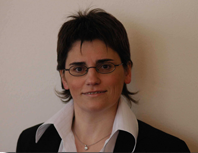
\includegraphics[width=0.9\fwidth]{../figures/samarati}
      \caption{Samarati}
    \end{subfigure}
    \hspace{0.05\textwidth}
    \begin{subfigure}{0.45\textwidth}
      \centering
      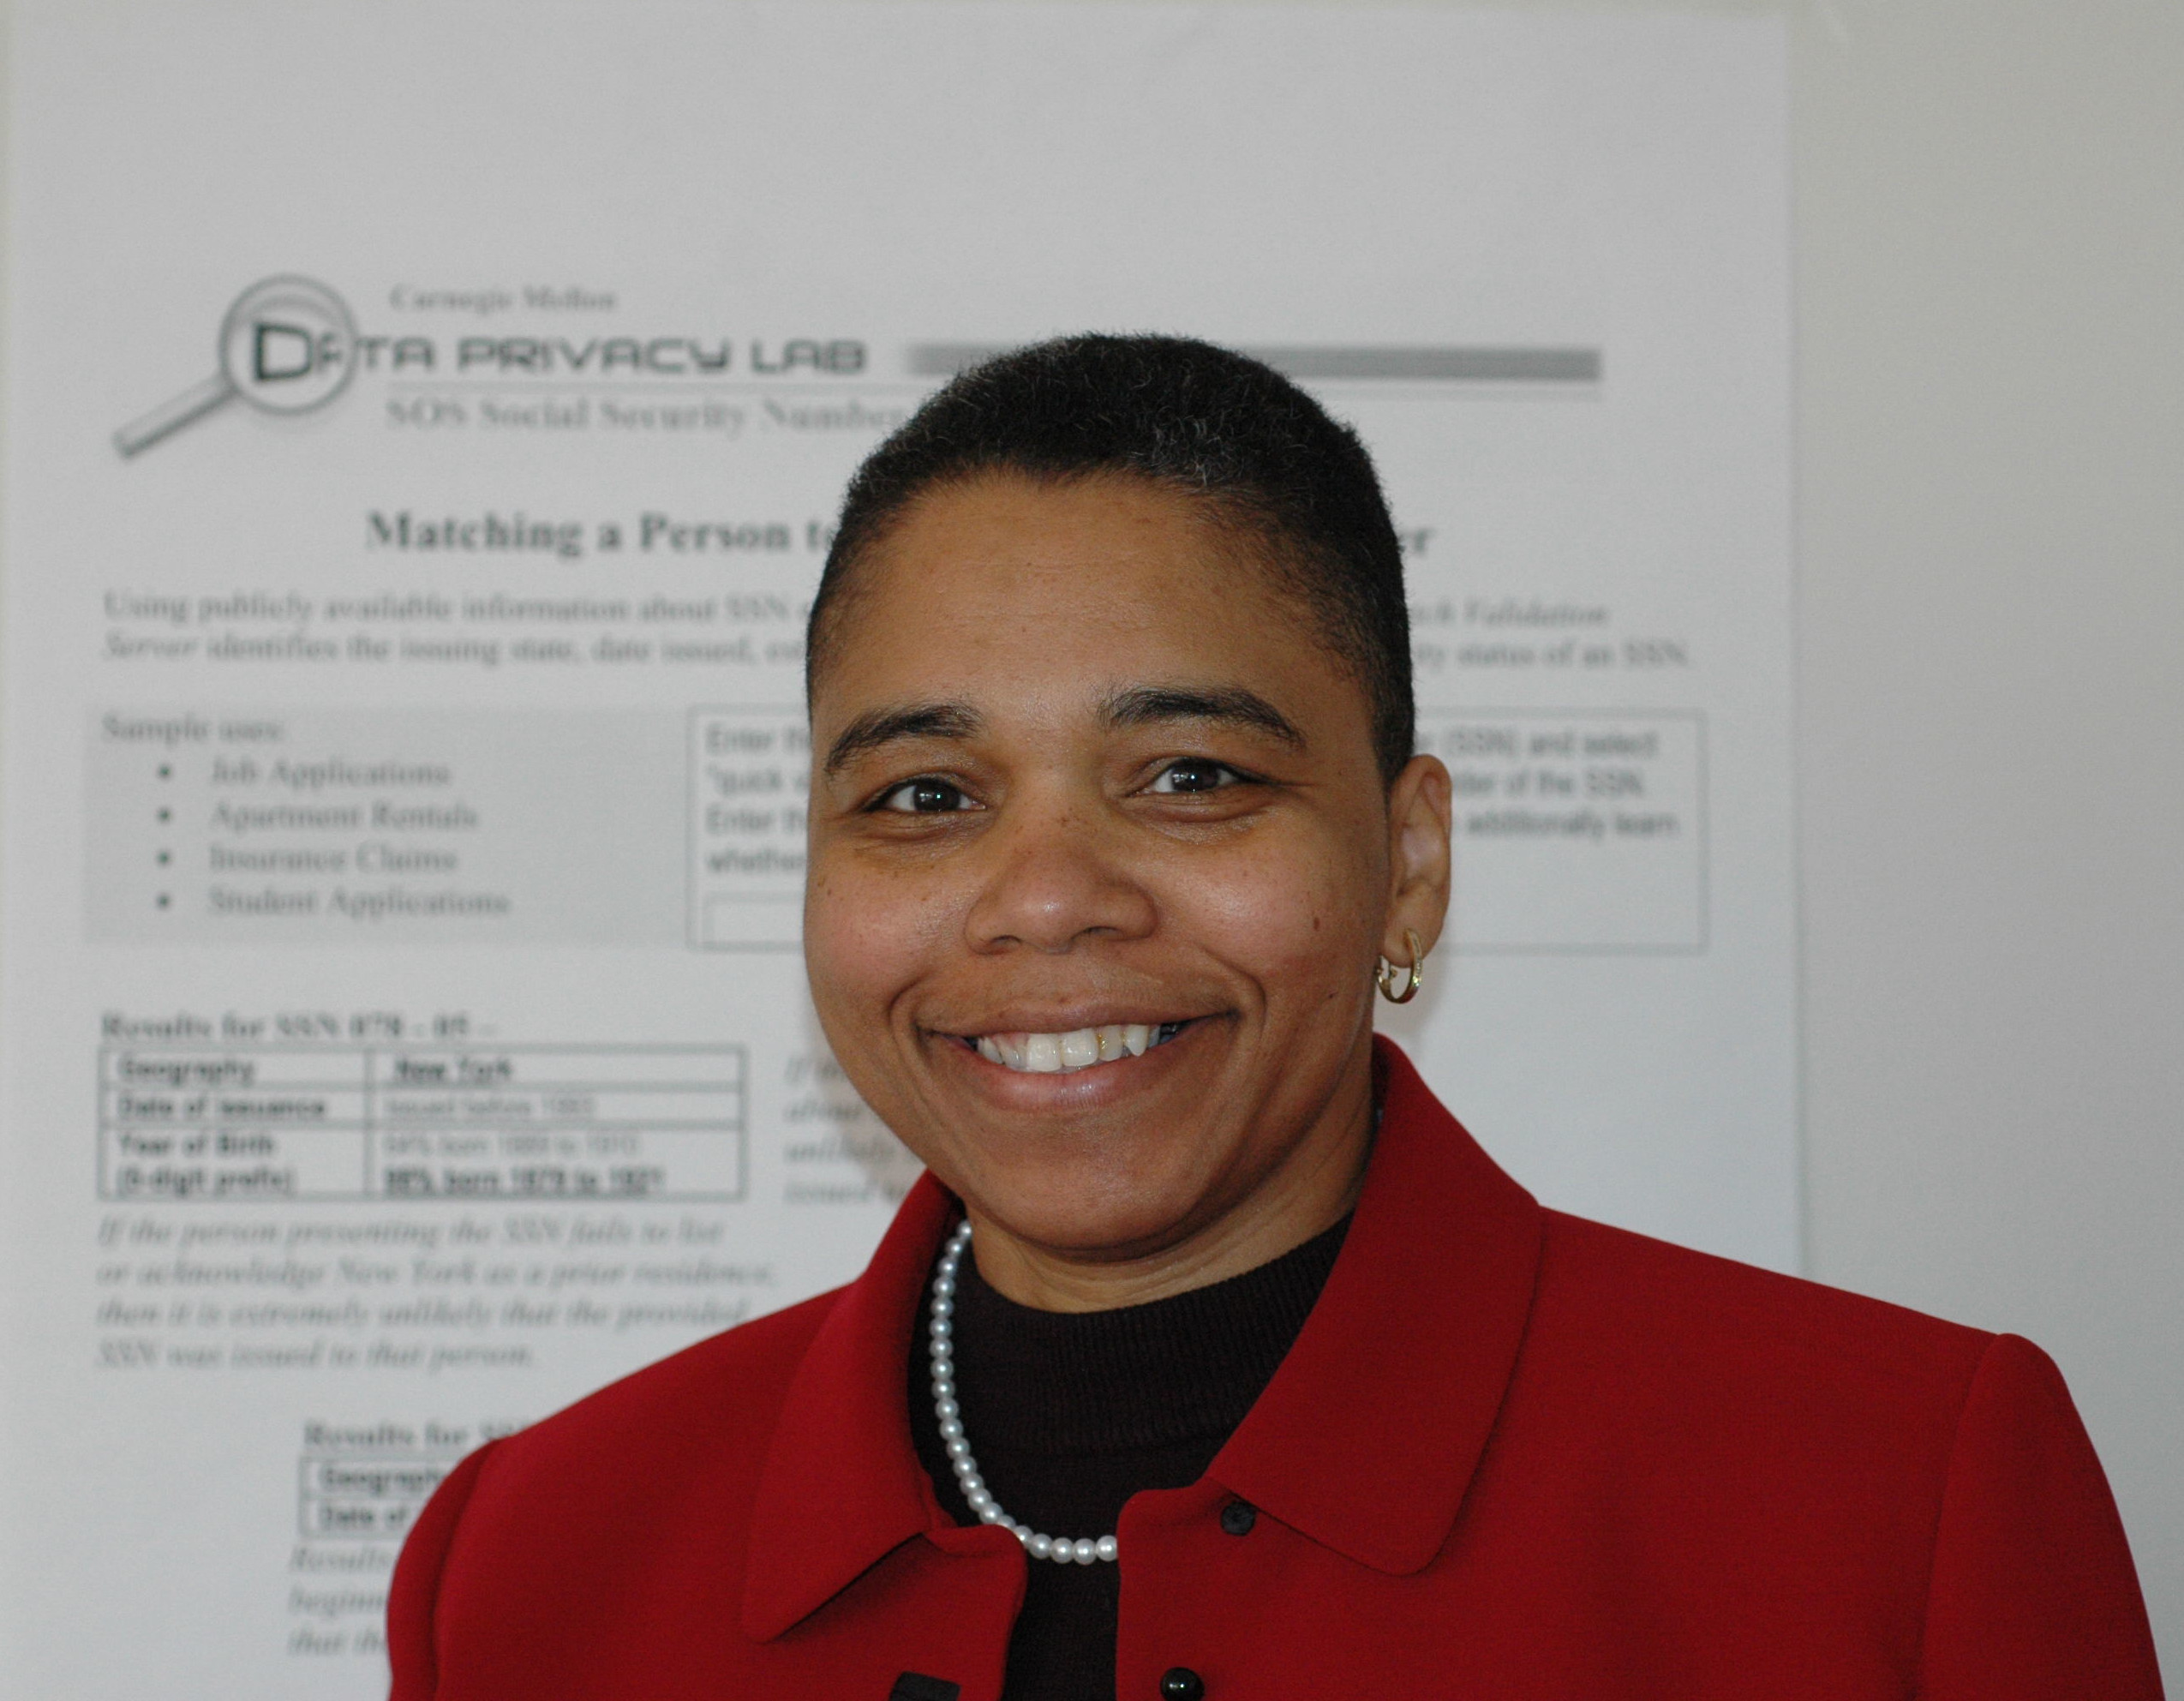
\includegraphics[width=0.9\fwidth]{../figures/sweeney}
      \caption{Sweeney}
    \end{subfigure}
  \end{figure}
  \only<article>{The concept of $k$-anonymity was introduced
    by~\citet{samarati1998protecting} and provides some guarantees
    against inferring personal information from a single
    database. This requires the analyst to first determine the
    variables of interest (which should not be modified), and then
    determine which variables are \emph{quasi-identifiers}, i.e. they
    could be potentially used to identify somebody in the database.}
  \alert{It's the analyst's job to define quasi-identifiers.} However, in general all variables should be considered quasi-identifiers.
  \begin{definition}[$k$-anonymity]
    A database provides $k$-anonymity if for every person in the
    database is indistinguishable from $k-1$ persons with respect to
    \emph{quasi-identifiers}.
  \end{definition}
  \only<article>{This hope is that, if the database satisfies
    $k$-anonymity it can be safely released, without revealing any
    private information directly. As you can see, the definition of
    $k$-anonymity relates to the algorithm \emph{output}, and not the
    algorithm itself. Because of this, it is not possible to give
    formal guarantees that hold generally for a $k$-anonymous
    database, as the result of the process does not tell us anything
    about how much information it conveys about the original input.

    But first, let us walk through an extended example to explain the
    concept.}
\end{frame}

\begin{frame}
  \frametitle{$k$-anonymity example}
  \only<article>{
    In particular, let us say that the analyst simply wants to calculate some statistics about how different professions correlate with age, weight, height and where people live. Some areas of the country might produce more politicians, for example. And taller people may be more successful in politics. The initial data collected might look like the table below. It was obvious to the analyst, that even if he did remove all the names, somebody knowing where A. B. Student lived and saw the table would have little trouble recognising them.
  }

  \only<1>{
    \begin{table}[H]
      \centering
      \begin{tabular}{l|l|l|l|l|l|l}
        Birthday & Name & Height  & Weight & Age & Postcode & Profession\\
        \hline
        06/07 & Li Pu & 190 & 80 & 65 & 1001 & Politician\\
        06/14 & Sara Lee & 185 & 110 & 67 & 1001 & Rentier\\
        06/12 & Nikos Karavas & 180 & 82 & 72+ & 1243 & Politician\\
        01/01 & A. B. Student & 170 & 70 & 52 & 6732 & Time Traveller\\
        05/08 & Li Yang & 175 & 72 & 35 & 6910 & Politician
      \end{tabular}
      \caption{1-anonymity.}
    \end{table}

  }
  \only<presentation>{
    \only<2>{
      \begin{tabular}{l|l|l|l|l|l|l}
        Birthday & Name & Height  & Weight & Age & Postcode & Profession\\
        \hline
        06/07 &  & 190 & 80 & 60+ & 1001 & Politician\\
        06/14 &  & 185 & 110 & 60+ & 1001 & Rentier\\
        06/12 &  & 180 & 82 & 60+ & 1243 & Politician\\
        01/01 &  & 170 & 70 & 40-60 & 6732 & Time Traveller\\
        05/08 &  & 175 & 72 & 30-40 & 6910 & Politician
      \end{tabular}
      1-anonymity
    }

    \only<3>{
      \begin{tabular}{l|l|l|l|l|l|l}
        Birthday & Name & Height  & Weight & Age & Postcode & Profession\\
        \hline
        06/07 &  & 180-190 & 80+ & 60+ & 1* & Politician\\
        06/14 &  & 180-190 & 80+ & 60+ & 1* & Rentier\\
        06/12 &  & 180-190 & 80+ & 60+ & 1* & Politician\\
        01/01 &  & 170-180 & 60-80 & 20-60 & 6* & Time Traveller\\
        05/08 &  & 170-180 & 60-80 & 20-60 & 6* & Politician
      \end{tabular}
      1-anonymity
    }
  }

  \only<article>{After thinking about it for a bit, the analyst decides to remove the birthday and name, and broadly categorise people according to their height in increments of 10cm, the weight in increments of 20cm, and keep just the first digit of the postcode. Now that looked much more reasonable. Still, somebody that knows that Li Yang and A. B. Student are in the table, as well as their postcodes, and they also know that Li Yang is a politician, can infer that A. B. Student is a Time Traveller.}
  \only<4>{
    \begin{table}[H]
      \centering
      \begin{tabular}{l|l|l|l|l|l|l}
        Height  & Weight & Age & Postcode & Profession\\
        \hline
        180-190 & 80+ & 60+ & 1* & Politician\\
        180-190 & 80+ & 60+ & 1* & Rentier\\
        180-190 & 80+ & 60+ & 1* & Politician\\
        170-180 & 60-80 & 20-60 & 6* & Time Traveller\\
        170-180 & 60-80 & 20-60 & 6* & Politician
      \end{tabular}
      \caption{2-anonymity: the database can be partitioned in sets of at least 2 records}
    \end{table}
  }


  \only<article>{However, with enough information, somebody may still
    be able to infer something about the individuals. In the example
    above, it remains true that if somebody knows that both
    A. B. Student and Li Yang are in the database, as well as their
    postcodes, as well as that Li Yang is a politician, they can infer
    A. B. Student's profession.  Fortunately, there is a way to
    protect individual information from adversaries with arbitrary
    side-information. This is given by differential privacy.  }
\end{frame}



\section{Differential privacy}
\label{sec:differential-privacy}
\only<article>{ This section introduces one of the main tools for
  giving formal guarantees about the privacy of any algorithm ran on
  a dataset, \emph{differential privacy}. This will provide
  individual-level privacy, in the sense that an algorithm that is
  differentially private guarantees that no adversary can
  significantly increase their knowledge about any particular
  individual by observing the algorithm's output. This is
  independent of the adversary's existing knowledge, or
  computational power. }

\only<article>{While $k$-anonymity can protect against specific
  re-identification attacks when used with care, it says little about
  what to do when the adversary has a lot of knowledge. For example,
  if the adversary knows the data of everybody that has participated
  in the database, it is trivial for them to infer what our own data
  is. For some particularly sensitive datasets, we may want for the
  adversary to be unable to tell whether or not your data was part of
  the base. Differential privacy offers protection against adversaries
  with unlimited side-information or computational power. Intuitively,
  an algorithmic computation is differentially-private if an adversary
  cannot distinguish two ``neighbouring'' databases based on the result
  of the computation. Informally, two databases are neighbours when
  they are identical apart from the data of one person. A
  differentially private algorithm, because of its randomness, makes
  it impossible for somebody to tell from the algorithm's output
  whether any specific individual's data was in the database. }

\begin{frame}
  \begin{figure}[H]
    \centering
    \begin{tikzpicture}[node distance=0.4\textwidth]
      \node[label=left:$x$] at (0,0) (data) {\includegraphics[width=0.1\columnwidth]{../figures/medical}};

      \node[label=$x_1$] at (-2,3)(patient1) {\includegraphics[width=0.05\columnwidth]{../figures/me-recent}};
      \uncover<3->{
        \node[label=$x_2$] at (2,3) (patient2) {\includegraphics[width=0.1\columnwidth]{../figures/judge}};
      }
      \uncover<4->{
        \node[label=$a$] at (4,0)   (statistics) {\includegraphics[width=0.2\columnwidth]{../figures/coronary-disease}};
      }
      \uncover<2->{
        \draw[->] (patient1) -- (data);
      }
      \uncover<3->{
        \draw[->] (patient2) -- (data);
      }
      \uncover<4->{
        \draw[->] (data) -- node[above]{$\pol$} (statistics);
      }
      \uncover<5->{
        \draw[line width=5, red, ->] (statistics) -- (patient2);
      }
    \end{tikzpicture}
    \caption{If two people contribute their data $x = (x_1, x_2)$ to a medical database, and an algorithm $\pol$ computes some public output $a$ from $x$, then it should be hard infer anything about the data from the public output.}
    \label{fig:privacy-data}
  \end{figure}
  \only<article>{ Consider the example given in
    Figure~\ref{fig:privacy-data}, where two people contribute their
    data to a medical database. The $i$-th individual contributes data
    $x_i$, and the complete dataset is $x = (x_1, x_2)$. The algorithm
    $\pol$ defines a distribution over the set of possible outputs
    $a \in \CA$, with $\pol(a | x)$ being the probability that the
    algorithm outputs $a$ if the data is $x$.  If the algorithm was
    deterministic, then it might be possible for an adversary to
    invert the computation and obtain $x$ from $a$. 
    But even if that
    is not possible, maybe they can learn \emph{something} about the
    data from the output. In the section below, we will formalise this
    notion. }
  
\end{frame}

\begin{frame}
  \frametitle{Privacy desiderata}
  \only<article>{
    Consider a scenario where $n$ persons give their data $x_1, \ldots, x_n$ to an analyst. This analyst then performs some calculation on the data and publishes the result through a randomised algorithm $\pol$, where for any output $a$, and any dataset $x$, $\pol(a | x)$ is the probability that the algorithm generates $a$.
    The following properties are desirable from a general standpoint.

    \paragraph{Anonymity.} Individual participation in the study remains a secret. From the release of the calculations results, nobody can significantly increase their probability of identifying an individual in the database.

    \paragraph{Secrecy.} The data of individuals is not revealed. The release does not significantly increase the probability of inferring individual's information $x_i$.

    \paragraph{Side-information.} Even if an adversary has arbitrary side-information, he cannot use that to amplify the amount of knowledge he would have obtained from the release.

    \paragraph{Utility.} The released result has, with high probability, only a small error relative to a calculation that does not attempt to safeguard privacy.
  }
  \only<presentation>{
    We wish to calculate something on some private data and publish a \alert{privacy-preserving}, but \alert{useful}, version of the result.
    \begin{itemize}
    \item Anonymity: Individual participation remains hidden.
    \item Secrecy: Individual data $x_i$ is not revealed.
    \item Side-information: Linkage attacks are not possible.
    \item Utility: The calculation remains useful.
    \end{itemize}
  }
\end{frame}

\begin{frame}
  \begin{exampleblock}{The prevalence of drugs in sport}
    
    \only<article>{
      Let's say you need to perform a statistical analysis of the drug-use habits of athletes. Obviously, even if you promise the athlete not to reveal their information, you still might not convince them. Yet, you'd like them to be truthful. The trick is to allow them to randomly change their answers, so that you can't be \emph{sure} if they take drugs, no matter what they answer.
    }

    \only<presentation>{
      \begin{itemize}
      \item $n$ athletes
      \item Ask whether they have doped in the past year.
      \item Aim: calculate \% of doping.
      \item How can we get truthful / accurate results?
      \end{itemize}
      \only<1>{
        \alert{Write responses in class}
      }
    }
    \only<2->{
      \begin{groupactivity}{Algorithm for randomising responses about drug use}
        \begin{enumerate}
        \item Flip a coin.
        \item If it comes heads, respond truthfully. 
        \item Otherwise, flip another coin and respond \texttt{yes} if it comes heads and \texttt{no} otherwise.
        \end{enumerate}
      \end{groupactivity}
      \begin{exerciseblock}{Calculating the true rate of responses.}
        Assume that the observed rate of positive responses in a sample is $p$, that everybody follows the protocol, and the coin is fair. Then, what is the true rate $q$ of drug use in the population?
      \end{exerciseblock}
      
    }
  \end{exampleblock}
  \only<3->{
  }
  \onslide<3->{
    \only<presentation>{
      \begin{proof}[Solution]
        Since the responses are random, we will deal with expectations first
        \begin{align*}
          \E p
          &= \frac{1}{2} \times \frac{1}{2} + q \times \frac{1}{2}
            \uncover<4->{= \frac{1}{4} + \frac{q}{2}}
            \uncover<5->{\\
          q &= 2 \E p - \frac{1}{2}.}
        \end{align*}
        
      \end{proof}
    }
  }
  \only<article>{The problem with this approach, of course, is that we are effectively throwing away half of our data sources. In particular, if we repeated the experiment with a coin that came heads at a rate $\epsilon$, then our error bounds would scale as $O(1/\sqrt{\epsilon n})$ for $n$ data points.}
\end{frame}

\begin{frame}
  \only<article>{This algorithm is very specific: it assumes binary responses, and it uses a fair coin, which introduces a lot of noise.  Since the coin flips make the responses noisy, we may want to have some way of controlling it. In general, we want to consider an algorithm that takes data $x_1, \ldots, x_n$ from $n$ users transforms it randomly to $a_1, \ldots, a_n$ using the following mapping.}
  \begin{block}{The binary randomised response mechanism}
    \begin{definition}[Randomised response]
      The $i$-th user, whose data is $x_i \in \{0,1\}$ , responds with $a_i \in \{0, 1\}$ with probability
      \[
        \pol(a_i = j \mid x_i = k) = p,  \qquad  \pol(a_i = k \mid x_i = k) = 1 - p,
      \]
      where $j \neq k$.
    \end{definition}
  \end{block}
  \uncover<2->{Given the complete data $x$, the algorithm's output is $a = (a_1, \ldots, a_n)$.}
  \uncover<3->{Since the algorithm independently calculates a new value for each data entry, the output probability is
    \[
      \pol(a \mid x) = \prod_i \pol(a_i \mid x_i)
    \]
  } \only<article>{This mechanism satisfies the formal notion of
    $\epsilon$-differential privacy, which will be given in
    Definition~\ref{def:epsilon-dp}. In a more general setting, we may
    have multiple possible responses. While the algorithm can be
    trivially generalised to $n$-ary outputs, the special case of when
    the outputs are integers is deferred until later.}
\end{frame}

\begin{exampleblock}{The original randomised response mechanism~\cite{werner:1965}}
  As first proposed by~\citeauthor{werner:1965}, the mechanism distributes spinners to people. The spinner has a probability $p$ of landing on $A$ and $1 - p$ of landing on $B$. This can be easily arranged by having the corresponding areas to have the appropriate proportions. The interesting thing about this mechanism is that the responders must merely say whether or not the spinner landed on the group they identify with. They do \emph{not} have to reveal a group. This makes the mechanism feel like you are revealing less, even if it is just a special case of a general randomised response mechanism.
\end{exampleblock}

\begin{frame}
  \frametitle{What can we learn from the output?}

  \only<article>{ In the Bayesian setting, we can think of the
    adversary as having some prior belief $\bel(x_i)$, expressed as a
    probability distribution over the secret value of each individual.

    After the adversary observes the output, they can form
    a posterior belief $\bel(x_i \mid a_i)$, representing the
    information they collected. The following example quantifies the
    amount of information gained by the adversary.
  }
  \begin{example}
    For simplicity, consider only one individual, and let the
    adversary have a prior $\bel(x = 0) = 1 - \bel(x = 1)$ over the
    values of the true response of an individual. We use the
    randomised response mechanism with parameter $p$ and the
    adversary observes the randomised data $a = 1$ for that
    individual, then what is $\Pr^\pol_\bel(x = 1 \mid a = 1)$, assuming the
    adversary knows the mechanism?
  \end{example}
  \begin{proof}
    Bayes's theorem states that\footnote{If there are too many symbols for you, you can write Bayes theorem simply with $P(x | a) = P(a | x) P(x) / P(a)$.}
    \[
      \Pr^\pol_\bel(x \mid a) = \pol(a \mid x) \bel(x) / \Pr^\pol_\bel(a),
    \]
    where
    \[
      \Pr^\pol_\bel(a) = \sum_{x'} \pol(a \mid x') \bel(x').
    \]
    Let $q = \bel(x = 1)$. Then we have:
    \[
      \Pr^\pol_\bel(x = 1 \mid a = 1) = pq / [pq + (1-p)(1 - q)].
    \]
    It is particularly interesting to consider the case where $q = 1/2$. Then
    \[
      \Pr^\pol_\bel(x = 1 \mid a = 1) = p,
    \]
    so we only have limited evidence for whether $x=1$. Now consider the case where we have some arbitrary prior $q$, and $p=1/2$. This means that the output of the algorithm is completely random. Consequently:
    \[
      \bel(x = 1 \mid a = 1) = q = \bel(x=1).
    \]
    So, in this scenario we learn nothing from the algorithm's output.
  \end{proof}
\end{frame}


\begin{frame}
  \frametitle{Differential privacy.}
  \only<presentation>{
    \includegraphics[width=0.2\textwidth]{../figures/dwork} \hspace{1em}
    \includegraphics[width=0.2\textwidth]{../figures/mcsherry} \hspace{1em}
    \includegraphics[width=0.2\textwidth]{../figures/nissim} \hspace{1em}
    \includegraphics[width=0.2\textwidth]{../figures/smith}
  }
  \only<article>{Now let us take a look at a way to characterise the  the inherent privacy properties of algorithms. This is called differential privacy, and it can be seen as a bound on the information an adversary with arbitrary power or side-information could extract from the result of a computation $\pol$ on the data. For reasons that will be made clear later, this computation has to be stochastic.}
  \begin{theoryblock}{$\epsilon$-Differential Privacy}
    \begin{definition}
      \label{def:epsilon-dp}
      A stochastic algorithm $\pol : \CX \to \Simplex(\CA)$, where $\CX$
      is endowed with a neighbourhood relation $N$, is said to be
      $\epsilon$-differentially private if
      \begin{equation}
        \label{eq:epsilon-dp}
        \left|\ln \frac{\pol(A \mid x)}{\pol(A \mid x')}\right| \leq \epsilon , \qquad \forall x N x', \quad A \subset \CA.
      \end{equation}
    \end{definition}
  \end{theoryblock}
  \only<article>{ This form is related to standard notions of
    statistical distance such as the KL divergence
    $\sum_a \ln \frac{\pol(a \mid x)}{\pol(a \mid x')} \pol(a \mid
    x)$.  However, the above inequality can be equivalently rewritten as
    \[
      \pol(A \mid x) \leq e^\epsilon \pol(A \mid x'). 
    \]
    Frequently (and particularly when $\CA$ is finite) we can also use
    $\pol(a \mid x)$ without any technical difficulties.  }

  \only<article>{Typically, algorithms are applied to
    datasets $x = (x_1, \ldots, x_n)$ composed of the data of $n$
    individuals. Thus, all privacy guarantees relate to the data
    contributed by these individuals.}
\end{frame}

\begin{frame}
  \frametitle{Neighbourhoods}

  \only<article>{
    Differential privacy guarantees that
    it is hard to distinguish neighbouring datasets. Hence, the
    definition of neighbourhood we use reflects what we want to
    protect. It makes sense to define neighbourhoods in terms of
    changes in one individual's data, because then an adversary cannot
    learn about the values of any particular individual.
    
    In this book we will use two definitions of neighbourhoods. The
    first is constructed so that the adversary cannot distinguish
    whether or not any particular individual's information is in the
    dataset. If not, then they cannot infer the individual's presence
    from the output of the algorithm.

  }
  \begin{definition}[Participation neighbourhood]
    If two datasets $x,x'$ are neighbours, then we write $xNx'$, and it holds that
    \[
      x = (x_1, \ldots, x_{i-1}, x_i, x_{i+1}, \ldots, x_n),
      \qquad
      x' = (x_1, \ldots, x_{i-1}, x_{i+1}, \ldots, x_n),
    \]
    for some $i$,  i.e. if one dataset is
    missing an element.
  \end{definition}
  \only<article>{ Under this neighbourhood relation, two datasets are
    neighbours if one contains the data of one individual, and the
    other does not, but they are otherwise the same. Then, if the
    algorithm is differentially private with respect to this
    neighbourhood, it is hard to tell if any single person's data has
    been used in the calculation.  This is an important concept if the
    participation in the dataset is itself sensitive. For example, if
    somebody is enlisted in study for experimental treatment of a rare
    disease, then the mere fact that they are part of the study is
    strong evidence that they have the disease.
    
    The second definition is slightly weaker. Here, two datasets are
    neighbours if they are identical, apart from the data of one
    individual, which is changed. It determines whether or not we can
    distinguish between different \emph{values} of individual data. If
    not, then they cannot infer whether the data submitted by the
    individual has a particular value.}
  \begin{definition}[Edit neighbourhood]
    We say that two datasets $x, x'$ are neighbours, and write $x N_e x'$ if
    \[
      x = (x_1, \ldots,  x_i, \ldots, x_n),
      \qquad
      x' = (x_1, \ldots, x'_i, \ldots,  x_n),
      \qquad
      x_i \neq x'_i.
    \]
    i.e. if one dataset has an altered element.
  \end{definition}
  \only<article>{ If $x,x'$ are 1-neighbours under the second
    definition, then they are 2-neighbours under the first
    definition. To see this, create a new dataset $\hat{x}$ from $x$,
    without the data of person $i$. Then $x N \hat{x}$ and
    $\hat{x} N x'$, since we can change the data of one person by
    removing the original data $x_i$ and then re-inserting the altered
    data $x'_i$. This is illustrated in the example below.}
\end{frame}



\begin{frame}
  \begin{exampleblock}{Neihgbourhood example}
    \only<article>{
      In this example, we have three datasets, $x, x'$ and $hat{x}$. In the second dataset, $\hat{x}$, the highlighted row in $x$ is missing. In the third dataset, $x'$, another row with the same name is added, but the height and weight are changed.
    }
    \begin{table}[H]
      \centering
      \begin{tabular}{l|l|l|l}
        Birthday & Name & Height  & Weight \\
        \hline
        06/07 & Li Pu & 190 & 80 \\
        06/14 & Sara Lee & 185 & 110  \\
        \alert<1>{06/12} & \alert<1>{John Smith} & \alert<1>{170} & \alert<1>{82} \\
        01/01 & A. B. Student & 170 & 70 \\
        05/08 & Li Yang & 175 & 72 
      \end{tabular}
      \caption{Data $x$}
    \end{table}
    \only<article>{
      In fact, $\hat{x}$ is obtained through a deletion from $x$. Of course, the operation can be reversed: $x$ can be obtained from an addition to $\hat{x}$.
    }
    \only<1>{
      \begin{table}[H]
        \centering
        \begin{tabular}{l|l|l|l}
          Birthday & Name & Height  & Weight \\
          \hline
          06/07 & Li Pu & 190 & 80 \\
          06/14 & Sara Lee & 185 & 110  \\
          01/01 & A. B. Student & 170 & 70 \\
          05/08 & Li Yang & 175 & 72 
        \end{tabular}
        \caption{$\hat{x}$, 1-Neighbour of $x$.}
      \end{table}
    }
    \only<article>{We can now instead add another row to $\hat{x}$, which will be similar to the row we had removed. This will have the effect of altering the original data in $x$.}
    \only<2>{
      \begin{table}[H]
        \centering
        \begin{tabular}{l|l|l|l}
          Birthday & Name & Height  & Weight \\
          \hline
          06/07 & Li Pu & 190 & 80 \\
          06/14 & Sara Lee & 185 & 110  \\
          06/12 & John Smith & \alert{180} & \alert{80} \\
          01/01 & A. B. Student & 170 & 70 \\
          05/08 & Li Yang & 175 & 72 
        \end{tabular}
        \caption{$x'$, 2-Neighbour of $x$.}
      \end{table}
      \only<article>{Since $x,x'$ only differ in the contents of a single row, they are edit-neighbours.}
    }
  \end{exampleblock}
\end{frame}

\begin{frame}
  \only<article>{ As we hinted earlier, the randomised response
    mechanism satisfies $\epsilon$-DP.  The $\epsilon$ parameter is
    dependent on $p$, with higher values giving a smaller $\epsilon$,
    and thus better privacy protection.}
  \begin{remark}
    The randomised response mechanism with $p \leq 1/2$ is
    $(\ln \frac{1 - p}{p})$-DP with respect to the edit neighbourhood
    $N_e$.
  \end{remark}
  \begin{proof}
    Consider $x = (x_1, \ldots, x_j,  \ldots, x_n)$, $x' = (x_1, \ldots, x'_j,  \ldots, x_n)$. Then
    \begin{align*}
      \pol(a \mid x)
      \uncover<2->{&= \prod_i \pol(a_i \mid x_i)}
                     \uncover<3->{\\ &= \pol(a_j \mid x_j) \prod_{i \neq j} \pol(a_i \mid x_i) }
                                       \uncover<4->{\\ &\leq \frac{1-p}{p} \pol(a_j \mid x'_j) \prod_{i \neq j} \pol(a_i \mid x_i) }
                                                         \uncover<5>{\\ &= \frac{1-p}{p} \pol(a \mid x')}
    \end{align*}
    \only<4>{$\pol(a_j = k\mid x_j = k) = 1 - p$ so the ratio is $\max\{(1-p)/p, p/(1 - p)\} \leq (1 - p)/p$ for $p \leq 1/2$.}
  \end{proof}

  \begin{groupactivity}{Moving to a new neighbourhood}
    Is the randomised-response mechanism for it to be differentially
    private with respect to the insertion-neighbourhood definition? If
    not, is it possible to modify it in order to satisfy that privacy
    definition?  \emph{Hint: The mechanism must be able to hide the
      participation of a single individual in the database.}
  \end{groupactivity}
  % Given this hint, the solution is obvious: The mechanism must
  % contain a non-identifying information aggregator. Let us take an
  % example, where individual responses are {0,1}. We can also add X,
  % as 'declined to respond'. Then the analyst will (by default) know
  % who has participated. Note that
  % $ln |p(a | x) / p(a|x')| < \epsilon$
  % requires that values of 0,1,X have non-zero probability for
  % everybody.  This is tricky, as typically the number of X will
  % depend on how many people do not participate, and the size of a
  % will be equal to the number of potential responders.


  
  \only<article>{Finally, it may be convenient to the look at
    neighbourhoods in terms of a distance between datasets. Let
    $\Naturals^{|\CX|}$ be the set of all possible dataset histograms,
    i.e. counts of different possible rows in each dataset. Then the
    distance between two datasets is simply the total difference in
    counts:
    \begin{definition}[Hamming distance between datasets]
      Consider two datasets, $\bx, \bx'$ with $n$ and $n'$ elements
      respectively. Then, we define their Hamming distance as:
      \begin{align}
        \|\bx - \bx'\|_1
        &= \sum_j |\sum_{i=1}^n \ind{x_i =j} - \sum_{i=1}^{n'} \ind{x_i =j}|
          = \sum_{j \in \CX}|n_j(\bx) - n_j(\bx')|,
      \end{align}
      where $n_j(\bx)$ is the number of elements in $\bx$ equal to $j$.
    \end{definition}
    Let us see how the Hamming distance relates to the two
    neighbourhoods we defined. In particular, $\|\bx - \bx'\|_1 = 1$
    if and only if $\bx N \bx'$.  To see this, notice that if $\bx'$
    has one row less than $\bx$, but is otherwise identical, then
    there is exactly one value $j$ for which
    $n_j(\bx) = n_j(\bx') + 1$, with $n_j(\bx) = n_j(\bx')$ otherwise.
    Consequently, $\|\bx - \bx'\|_1 = 1$. The reverse direction
    follows by contradiction: if the Hamming distance is one, then the
    two databases must differ in at least one element. If they differ
    in more, then their distance has to be larger than one.
    
    On the other hand, for the second neighbourhood definition, things
    are slightly different. There, we assume that $x_i \neq x'_i$ for
    one $i$. Without loss of generality, let us say that $x_i = j$ and
    $x'_i = k$, with $j \neq k$. Then $n_j(\bx) = n_j(\bx') + 1$ and
    $n_k(\bx') = n_k(\bx) + 1$. Consequently $\|\bx - \bx'\|_1 = 2$.
  }
\end{frame}


\section{The local and central privacy models}
\label{sec:local-central-dp}
\only<article>{ So far, we have only seen the concept of differential
  privacy applied as a method to generate a privatised version of a
  dataset. This can then be used to perform arbitrary
  computations. Typically, however, we want to perform some specific
  calculations on the data. Is it possible to compute things privately
  using the original data, but so that the result of the computation
  does not leak any information? Clearly this should depend somehow on
  the computation you wish to perform.

  For concreteness, let us assume that you have defined a function
  $f : \CX \to \CY$, which you wish to compute on arbitrary data
  $x \in \CX$. If you wish to preserve privacy, however, you need the
  computation to satisfy some formal guarantee like differential
  privacy. The simplest way to do this is by simply generating a
  dataset $a$ with a DP algorithm and then processing the data with
  the function we have already specified. This corresponds to the
  local privacy model.}


\begin{frame}
  \begin{block}{The local privacy model.}
    \only<presentation>{
      \begin{itemize}
      \item Individuals generate $a_i$ from $x_i$ using a DP policy $\pol(a_i | x_i)$.
      \item The analyst calculates $f(\ba)$.
      \end{itemize}
    }
    \only<article>{Given a function $f : \CX \to \CY$, and a set of
      individual data $\bx = (x_i)_{i=1}^n$, use a differentially
      private algorithm $\pol(\ba | \bx)$ to generate $\ba \in
      \CX$. Then output $f(\ba)$.}
  \end{block}

  \only<article>{ The advantage of the local model is that the
    calculation $f$ does not need to be modified. The individuals do
    not have to trust anybody, as they can modify their data
    locally. However, they must take care that the DP calculation is
    performed correctly.  }

  \only<article>{ Typically, in the local privacy model, the $i$-th
    individual's data $x_i$ is used to generate a private response
    $a_i$. This means that individual data is only available to a
    local private mechanism. This model allows us to publish a
    complete dataset of private responses.  In the central privacy
    model, the data $x$ is collected and the result $a$ is published
    by a \alert{trusted curator.}}
  
  \begin{block}{The central privacy model.}
    \only<presentation>{
      \begin{itemize}
      \item A \alert{trusted analyst} obtains $\bx$.
      \item She designs a DP policy $\pol(\ba \mid \bx)$ so that $\ba \approx f(\bx)$.
      \end{itemize}
    }
    \only<article>{A trusted curator obtains the data $\bx$ of all
      individuals and selects a DP policy $\pol(\ba \mid \bx)$ to generate
      the output $a$, so that $\ba \approx f(\bx)$.}
  \end{block}
  \only<article>{ The main advantage of the centralised model is that
    approximating $f$ with a differentially-private version can be much
    more accurate than simply using the original function with noisy
    data. However, obtaining such an approximation is not always easy.

    The dependency diagrams in Figures~\ref{fig:privacy-diagrams} shows
    how the output depends on the individual data, the non-private and
    private algorithm. 

  }
  
  \begin{figure}[H]
    \begin{subfigure}{0.3\textwidth}
      \centering
      \begin{tikzpicture}
        \node[RV] at (0,0) (x1) {$x_1$};
        \node[RV] at (0,1) (x2) {$x_2$};
        \node[RV] at (0,2) (xn) {$x_n$};
        \node[RV] at (2,1) (y) {$y$};
        \node[select] at (1,-1) (pol) {$f$};
        \draw[->] (x1) -- (y);
        \draw[->] (x2) -- (y);
        \draw[->] (xn) -- (y);
        \draw[->] (pol) -- (y);
      \end{tikzpicture}
      \caption{Non-private calculation}
      \label{fig:non-private}
    \end{subfigure}
    \begin{subfigure}{0.3\textwidth}
      \centering
      \begin{tikzpicture}
        \node[RV] at (0,0) (x1) {$x_1$};
        \node[RV] at (0,1) (x2) {$x_2$};
        \node[RV] at (0,2) (xn) {$x_n$};
        \node[RV] at (2,0) (a1) {$a_1$};
        \node[RV] at (2,1) (a2) {$a_2$};
        \node[RV] at (2,2) (an) {$a_n$};
        \draw[->] (x1) -- (a1);
        \draw[->] (x2) -- (a2);
        \draw[->] (xn) -- (an);
        \node[select] at (2,-1) (f) {$f$};
        \node[select] at (1,-1) (p) {$\pol$};
        \node[RV] at (3,1) (y) {$y$};
        \draw[->] (a1) -- (y);
        \draw[->] (a2) -- (y);
        \draw[->] (an) -- (y);
        \draw[->] (f) -- (y);
        \draw[->] (p) -- (a1);
        \draw[->] (p) -- (a2);
        \draw[->] (p) -- (an);
      \end{tikzpicture}
      \caption{Local privacy}
      \label{fig:local-privacy}
    \end{subfigure}
    \begin{subfigure}{0.3\textwidth}
      \centering
      \begin{tikzpicture}
        \node[RV] at (0,0) (x1) {$x_1$};
        \node[RV] at (0,1) (x2) {$x_2$};
        \node[RV] at (0,2) (xn) {$x_n$};
        \node[RV] at (2,1) (a) {$a$};
        \node[select] at (1,-1) (pol) {$\pol_f$};
        \draw[->] (x1) -- (a);
        \draw[->] (x2) -- (a);
        \draw[->] (xn) -- (a);
        \draw[->] (pol) -- (a);
      \end{tikzpicture}
      \caption{Central privacy}
      \label{fig:central-privacy}
    \end{subfigure}
    \caption{Non-privacy, local privacy, and centralised privacy models. In the first case, the value of $y$ depends directly on the function $f$ to be calculated, as well as the data $x$. In the local privacy model, noise is added to the individual data with a differentially private algorithm $\pol$, and the function is calculated on the output. In the central model, a stochastic version $\pol_f$ of the original function $f$ is calculated on the data.}
    \label{fig:privacy-diagrams}
  \end{figure}


  \begin{groupactivity}{Trust models.}
    Google uses a local privacy model to collect data from Android
    phone users. How does this compare to Google gathering data in the
    clear and then performing private computations? Who do the users
    have to trust? What are the privacy risks in either case?
  \end{groupactivity}
\end{frame}


\subsection{Properties of differential privacy.}
\begin{frame}

  \only<article>{
    \begin{remark}
      Any differentially private algorithm must be stochastic.
    \end{remark}

    To prove that this is necessary, consider the example of counting how many people take drugs in a competition. If the adversary only doesn't know whether you in particular take drugs, but knows whether everybody else takes drugs, it's trivial to discover your own drug habits by looking at the total. This is because in this case, $f(x) = \sum_i x_i$ and the adversary knows $x_i$ for all $i \neq j$. Then, by observing $f(x)$, he can recover $x_j = f(x) - \sum_{i \neq j} x_i$. Consequently, it is not possible to protect against adversaries with arbitrary side information without stochasticity.}
\end{frame}

\only<article>{ Randomness is also necessary in cryptography.  In that
  setting, Alice wants to communicate a message $x$ to Bob.  In a
  secret key cryptographic scheme, information theoretic security is
  achieved by making sure that the encrypted message $a$ comes from a
  uniform distribution $\pol(a | x)$. This is achieved by uniformly
  selecting a key and selecting an appropriate hash function }


\begin{frame}


  
  \only<article>{Depending on the DP scheme, each query answered may leak privacy. In particular, if we always respond with an $\epsilon$-DP mechanism, after $T$ queries our privacy guarantee is $T \epsilon$. There exist mechanisms that do not respond to each query independently, which can reduce the total privacy loss, but those are outside the scope of this chapter.}
  \only<presentation>{
    \begin{block}{Properties of $\epsilon$-DP algorithms}
      \begin{itemize}
      \item Composition: If $\pol_1, \pol_2$ are $\epsilon_1, \epsilon_2$-DP respectively, their composition is $(\epsilon_1 + \epsilon_2)$-DP.
      \item Post-processing: Any transformation of the output of an $\epsilon$-DP algorithm does not induce further privacy loss.
      \end{itemize}
    \end{block}
  }
  \begin{definition}[$T$-fold composition]
    In this privacy model, we compose a mechanism out of $T$ differential private mechanisms $\pol_1, \ldots, \pol_T$. This composition is fixed ahead of time.
    % The composition is \alert{adaptive}, in the sense that the next query is allowed to depend on the previous queries and their results.
  \end{definition}
  \begin{theorem}
    For any $\epsilon > 0$, the class of $\epsilon$-differentially private mechanism satisfy $T \epsilon$-differential privacy under $T$-fold composition. More generally, if each mechanism is $\epsilon_i$-DP, the composed mechanism is $\sum_{i=1}^T \epsilon_i$-DP.
  \end{theorem}

  \begin{theorem}[Post-processing]
    Let mechanism $\pi(a \mid x)$ be $\epsilon$-DP. Applying any transformation $f : A \to Y$ to the output of the mechanism to obtain $y = f(a)$, results in another $\epsilon$-DP mechanism.
  \end{theorem}

  \only<presentation>{
    \begin{alertblock}{Composition}
      If we answer $T$ queries with an $\epsilon$-DP mechanism, then our cumulative privacy loss is $\epsilon T$.
    \end{alertblock}
  }
  \only<article>{The composition theorem is a very useful tool, as it allows us to create new mechanisms that are composed of simpler parts. As a first example, we can look at how we can use it to create a randomised response algorithm when the respondents provide multiple attributes.}

  \begin{exampleblock}{Randomised response for multiple attributes.}
    \only<article>{Up to now we have been discussing the case where each individual only has one attribute. However, in general each individual $t$ contributes multiple data $x_{t.i}$, which can be considered as a row $\bx_t$ in a database. Then the mechanism can release each $a_{t,i}$ independently.}
    
    For $n$ users and $k$ attributes, if the release of each attribute $i$ is $\epsilon$-DP then 
    the data release is $k \epsilon$-DP. Thus to get $\epsilon$-DP overall,  we need $\epsilon / k$-DP per attribute.
    
    \only<article>{The result follows immediately from the composition theorem. We can see each attribute release as the result of an individual query. More generally, if each attribute $i$ is released with an $\epsilon_i$-DP mechanism, the overall mechanism is $\sum_i \epsilon_i$-DP.}
  \end{exampleblock}

\end{frame}


\begin{frame}
  
  \begin{exerciseblock}{Differential privacy from a Bayesian viewpoint.}
    \only<article>{Bayesian inference offers a simple way to explain the meaning of differential privaacy. Intuitively, using the Bayesian formalism, we can show that, no matter what prior knowledge the adversary has, they cannot infer a lot from the private release. We are specifically interested in adversary knowledge about the dataset, before and after the mechanism's release. In particular, assume that the adversary knows that the data is either $\bx$ or $\bx'$. For concreteness, assume the data is either }
    \[
      \bx = (x_1, \ldots, x_j = 0, \ldots,  x_n)
    \]
    \only<article>{where $x_i$ is the data of person $i$, or the alternative dataset:}
    \[
      \bx' = (x_1, \ldots, x'_j=1, \ldots, x_n).
    \]
    \only<article>{In other words, the adversary knows the data of all people apart from one, the $j$-th person. They only need to dinstiguish one possible value from another. Without loss of generality, we can model the adversary as having some arbitrary prior belief}
    \[
      \bel(\bx) = 1 - \bel(\bx')
    \]
    \only<article>{for the two cases. Assume the adversary knows
      the output $a$ of a mechanism $\pol$.}
    \only<presentation>{
      \onslide<2->{
        \[
          a_t, \qquad \pol(a_t \mid \bx_t) \Rightarrow
          \begin{cases}
            \pol(a_t \mid \bx_t = \bx)\\
            \pol(a_t \mid \bx_t = \bx')
          \end{cases}
        \]
      }
    }
    What can we say about the posterior distribution of the adversary $\bel(\bx \mid a, \pol)$ after having seen the output, if $\pol$ is $\epsilon$-DP? How does it depend on $\epsilon$?
  
  \only<article>{
    \begin{proof}[Solution]
      We can write the adversary posterior as follows.
      \begin{align}
        \Pr^\pol_\bel(\bx \mid a)
        &=
          \frac{\pol(a  \mid \bx) \bel(\bx)}
          {\pol(a  \mid \bx) \bel(\bx) + \pol(a  \mid \bx') \bel(\bx')}
        \\
        &\geq
          \frac{\pol(a  \mid \bx) \bel(\bx)}
          {\pol(a  \mid \bx) \bel(\bx) + \pol(a  \mid \bx) e^\epsilon \bel(\bx')} \tag{from DP definition}
        \\
        &=
          \frac{\bel(\bx)}
          {\bel(\bx) +  e^\epsilon \bel(\bx')}.
      \end{align}
      Note that $\pol(a \mid \bx) \leq e^\epsilon \pol(a \mid \bx')$ and conversely $\pol(a \mid \bx') \leq e^\epsilon \pol(a \mid \bx)$.
      We can also then bound the quantity from above:
      \[
        \Pr^\pol_\bel(\bx \mid a) \leq  \frac{\bel(\bx)} {\bel(\bx) +  e^{-\epsilon} \bel(\bx')}.
      \]
      Consequently, $\lim_{\epsilon \to 0} \Pr^\pol_\bel(\bx \mid a) = \beta(\bx)$, hence the information gained by the adversary is bounded by the prior and the information loss $\epsilon$.
    \end{proof}
  }
  \end{exerciseblock}    

  
\end{frame}





\section{The Laplace mechanism}
\label{sec:laplace-mechanism}
\begin{frame}
  \only<article>{ Many times we already have a function
    $f : \CX \to \Reals$ we want to calculate on data, and we would
    like to make the function preserve privacy. This clearly falls
    within the \emph{central privacy} model: The analyst has access to
    the data and function, and wishes for the algorithm generating the
    final output to be private.  One solution, that can satisfy
    differential privacy, is to add noise to the function's output. We
    start by first calculating the value of the function for the data
    we have, $f(x)$, and then we add some random noise $\omega$, hence
    our calculation is random:
    \[
      a = f(x) + \omega.
    \]
    The amount and type of noise added, together with the smoothness of the function $f$, determine the amount of privacy we have. One of the simplest noise-adding mechanisms is to add zero-mean Laplace noise. Then we write $\omega \sim \Laplace(\lambda)$.\footnote{When unspecified, the mean parameter is assumed to be zero.} The mechanism is defined below.
  }
  \begin{definition}[The Laplace mechanism]
    For any function $f : \CX \to \Reals$, the output $a$ of the mechanism is sampled from a Laplace distribution with mean $f(x)$ and scaling parameter $\lambda$, i.e.
    \begin{equation}
      \label{eq:laplace-mechanism}
      \pol(a \mid x) = \Laplace(f(x), \lambda).
    \end{equation}
    The probability density function of the Laplace distribution with mean $\mu$ and scaling $\lambda$ is given by:
    \[
      p(\omega \mid \mu, \lambda) = \frac{1}{2 \lambda} \exp\left(-\frac{|\omega - \mu|}{\lambda}\right).
    \]
    and has mean $\mu$ and variance $2 \lambda^2$.
  \end{definition}
\end{frame}

\begin{frame}
  \begin{exampleblock}{The Laplace mechanism for averages}
    \only<article>{Here we have $n$ individuals for which we wish to calculate the average salary.}
    \begin{itemize}
    \item The $i$-th person receives salary $x_i$
    \item We wish to calculate the average salary in a private manner.
    \end{itemize}
    \only<article>{We can do this in two ways. By using a DP mechanism on each individual salary and then calculating the average, or by first calculating the average and then applying a DP mechanism to the result. In particular, we can add try adding Laplace noise in both cases.}

    \textbf{The local model.}
    \only<article>{In this case, $\pol(a \mid x)$ is obtained by independent Laplace noise $\omega_i$ for each individual:}
    \begin{itemize}
    \item Obtain $y_i = x_i + \omega_i$, where $\omega_i \sim \Laplace(\lambda)$.
    \item Return $a = n^{-1} \sum_{i=1}^n y_i$.
    \end{itemize}

    \textbf{The centralised model.}
    \only<article>{In this case, $\pol(a \mid x)$ is obtained by averaging first and adding noise later.}
    \begin{itemize}
    \item Calcualte $y = n^{-1} \sum_{i=1}^n x_i$.
    \item Return $a = y + \omega$, where $\omega \sim \Laplace(\lambda')$.
    \end{itemize}
    \only<article>{We must tune $\lambda, \lambda'$ appropriately in to obtain the needed $\epsilon$-DP guarantee.}
  \end{exampleblock}


  \begin{figure}
    \centering
    \begin{tikzpicture}
      \node[RV] at (0,0) (x1) {$x_1$};
      \node[RV] at (0,1) (x2) {$x_2$};
      \node[RV] at (0,2) (xn) {$x_n$};
      \node[RV] at (2,1) (y) {$y$};
      \node[select] at (1,-1) (f) {$f$};
      \node[select] at (3,-1) (pol) {$\pol$};
      \node[RV] at (4,1) (a) {$a$};
      \draw[->] (f) -- (y);
      \draw[->] (x1) -- (y);
      \draw[->] (x2) -- (y);
      \draw[->] (xn) -- (y);
      \draw[->] (y) -- (a);
      \draw[->] (pol) -- (a);
    \end{tikzpicture}
    \caption{Laplace mechanism}
  \end{figure}
  
  \only<article>{In the centralised privacy model, the non-private calculation directly outputs $y = f(x)$. We can approximate this with a DP calculation with distribution $\pol(a \mid x)$. The Laplace mechanism does so by first calculating $y = f(x)$ and then generating $\pol(a \mid y)$ so that $\E_\pol[a \mid x] = f(x)$.}


  \only<article>{Let us now talk about how the Laplace mechanism that can be used both in the centralised and local model when $\CX \subset \Reals^n$ and $\CY \subset \Reals$.}
\end{frame}

\begin{frame}
  \frametitle{DP properties of the Laplace mechanism}
  \only<article>{To use the Laplace mechanism in the centralised setting, we must relate it to a specific function $f$ that we wish to compute. In particular, the mecnahism works by adding noise to the output of the function $f$ in a carefully calibrated manner so that we achieve exactly $\epsilon$-differential privacy. }
  \begin{definition}[Sensitivity]
    The sensitivity of a function $f$ is
    \[
      \sensitivity{f} \defn \sup_{x N x'} |f(x) - f(x')|
    \]
    \only<article>{
      If we define a metric $d$, so that $d(x, x') = 1$ for $x N x'$, then:
      \[
        |f(x) - f(x')| \leq \sensitivity{f} d(x, x'),
      \]
      i.e. $f$ is $\sensitivity{f}$-Lipschitz with respect to $d$.
    }
  \end{definition}
  \begin{example}
    If $f: \CX \to [0, B]$, e.g. $\CX = \Reals$ and $f(x) = \min\{B, \max\{0, x\}\}$, then
    \onslide<2->{
      $\sensitivity{f} = B$.
    }
  \end{example}
  \onslide<3->{
    \begin{example}
      If $f: [0,B]^n \to [0,B]$ is
      $f = \frac{1}{n} \sum_{t=1}^n x_t$,
      then
      \onslide<4->{
        $\sensitivity{f} = B/n$.
      }
    \end{example}
    \only<article>{
      \begin{proof}
        Consider two neighbouring datasets $x, x'$ differing in example $j$. Then
        \[
          f(x) - f(x')
          = \frac{1}{n}\left[f(x_j) - f(x'_j)\right]
          \leq \frac{1}{n}\left[B - 0\right]
        \]
      \end{proof}
    }
  }
\end{frame}
\begin{frame}
  \begin{theorem}
    The Laplace mechanism on a function $f$ with sensitivity $\sensitivity{f}$, ran with $\Laplace(\lambda)$ is $\sensitivity{f} / \lambda$-DP. Consequently, if the Laplace mechanism is ran with $\lambda = \sensitivity{f} / \epsilon$, then it is $\epsilon$-DP. 
  \end{theorem}
  \begin{proof}
    \begin{align*}
      \frac{\pol(a \mid x)}{\pol(a \mid x')}
      &=
        \frac{e^{|a - f(x')|/\lambda}}{e^{|a - f(x)|/\lambda}}
        \leq
        \frac{e^{|a - f(x)|/\lambda + \sensitivity{f}/\lambda}}{e^{|a - f(x)|/\lambda}}
        = e^{\sensitivity{f} / \lambda}
    \end{align*}
    \only<article>{
      The first step follows from the definition of the Laplace mechanism. The inequality follows from the fact that for  $x N x'$, we have $|f(x) - f(x')| \leq \sensitivity{f}$. In particular, 
      \begin{enumerate}[(a)]
      \item If $f(x') - a \geq 0$ then
        \[|f(x') - a| = f(x') - a  \leq \sensitivity{f} + f(x) - a \leq L + |a - f(x)|,\]
        as $f(x') \leq f(x) + \sensitivity{f}$ from the Lipschitz property.
      \item If $f(x') - a < 0$ then
        \[
          |f(x') - a| = a - f(x')   \leq \sensitivity{f} - f(x) + a \leq L + |a - f(x)|,
        \]
        as $-f(x') \leq \sensitivity{f} - f(x)$.
      \end{enumerate}
      Replacing into the exponential gives us the required inequality. The final result is obtained with elementary algebra.
    }
  \end{proof}

  \begin{exampleblock}{DP properties of the average in the local and central model.}
    What is the effect of applying the Laplace mechanism in the local
    versus centralised model?  \only<article>{ Let us continue the
      average example.  Here let us assume $x_i \in [0, B]$ for all
      $i$.
      \begin{block}{The Laplace mechanism in the local privacy model}
        The sensitivity of the individual data is $B$, so to obtain $\epsilon$-DP we need to use $\lambda = B / \epsilon$. The variance of each component is $2(B/\epsilon)^2$, so the total variance is $2B^2/\epsilon^2 n$.
      \end{block}
      \begin{block}{The Laplace mechanism in the centralised privacy model}
        The sensitivity of $f$ is $B / n$, so we only need to use $\lambda = \frac{B}{n \epsilon}$. The variance of $a$ is $2(B / \epsilon n)^2$. 
      \end{block}
      Thus the two models have a significant difference in the variance of the estimates obtained, for the same amount of privacy. While the central mechanism has variance $O(n^{-2})$, the local one is $O(n^{-1})$ and so our estimates will need much more data to be accurate under this mechanism. In particular, we need square the amount of data in the local model as we need in the central model. Nevertheless, the local model may be the only possible route if we have no specific use for the data.
    }
    
  \end{exampleblock}
\end{frame}

\section{Interactive data access.}
\only<article>{
  In a lot of applications, we cannot pre-define the computation that we want to perform. After we have collected the data, we need to be perform an adaptive data analysis.  This requires performing a sequence of computations on the data, where the result of one computation determines what computation we will do next.

  We can think of this as performing queries to the database. You may
  be familiar with database access languages such as SQL, where you
  ask a question such as ``what is the sum of the attribute
  \texttt{age} in table \texttt{students}?''and obtain the exact sum
  back. It is possible to answer such queries through a differentially
  private mechanism. However, the more queries you answer, the more
  you reveal about the original data. In addition, since an adversary
  may be cleverly adjusting the queries to more efficiently discover a
  secret, we need the concept of adaptive composition.
}
\begin{frame}
  \only<presentation>{
    \frametitle{Databases}
    \begin{example}[Typical relational database in a tax office]
      \begin{table}[H]
        \centering
        \begin{tabular}{l|l|l|l|l|l|l}
          ID & Name &  Salary & Deposits & Age & Postcode & Profession\\
          \hline
          1959060783 & Li Pu & 150,000 & 1e6 & 60 & 1001 & Politician\\
          1946061408 & Sara Lee & 300,000 & -1e9 & 72 & 1001 & Rentier\\
          2100010101 & A. B. Student & 10,000 & 100,000 & 40 & 1001 & Time Traveller
        \end{tabular}
      \end{table}
    \end{example}
    \only<1>{
      \begin{block}{Database access}
        \begin{itemize}
        \item When owning the database: Direct look-up.
        \item When accessing a server etc: Query model.
        \end{itemize}
      \end{block}
    }
  }
  \only<2>{
    \begin{figure}[H]
      \centering
      \begin{tikzpicture}
        \node[rectangle] at (0,0) (python) {Python program};
        \node[rectangle] at (8,0) (database) {Database System};
        \draw[thickarrow, bend right]   (python) to node[black]{Query} (database) ;
        \draw[thickarrow, bend right]   (database) to node[black]{response} (python) ;
      \end{tikzpicture}
      \label{fig:database-access}
      \caption{Database access model}
    \end{figure}
  }
  
\end{frame}

\only<presentation>{
  \begin{frame}
    \frametitle{SQL: A language for database access}
    \begin{block}{Creating and filling tables}
      \begin{itemize}
      \item \texttt{CREATE TABLE table-name (column1, column2)}
        \only<article>{Create a new table}
      \item \texttt{INSERT INTO table-name VALUES ('value1', 'value2')}
        \only<article>{Add specific values into a table}
      \item \texttt{INSERT INTO table-name VALUES (?, ?), variable}
        \only<article>{Fill in values from a variable}
      \end{itemize}
    \end{block}

    \begin{example}{Database creation}
      \url{src/privacy/database-creation.py}
      \\
      \url{src/privacy/database-access.py}
    \end{example}
  \end{frame}
  \begin{frame}
    \frametitle{Queries in SQL}
    \begin{block}{The \texttt{SELECT} statement}
      \begin{itemize}
      \item \texttt{SELECT column1, column2 FROM table;}
        \only<article>{This selects only some columns from the table}
      \item \texttt{SELECT * FROM table;}
        \only<article>{This selects all the columns from the table}
      \end{itemize}
    \end{block}

    \begin{block}{Selecting rows}
      \texttt{SELECT * FROM table WHERE column = value;}
    \end{block}

    \begin{exampleblock}{Arithmetic queries}
      \only<article>{Here are some example SQL statements}
      \begin{itemize}
      \item  \texttt{SELECT COUNT(column) FROM table WHERE condition;}
        \only<article>{This allows you to count the number of rows matching \texttt{condition}}
      \item  \texttt{SELECT AVG(column) FROM table WHERE condition;}
        \only<article>{This lets you to count the number of rows matching \texttt{condition}}
      \item  \texttt{SELECT SUM(column) FROM table WHERE condition;}
        \only<article>{This is used to sum up the values in a column.}
      \end{itemize}
    \end{exampleblock}

  \end{frame}
}

\only<presentation>{
  \begin{frame}
    \begin{figure}[H]
      \centering
      \begin{tikzpicture}
        \node[rectangle] at (0,0) (python) {Python program};
        \node[rectangle] at (8,0) (database) {Database System};
        \draw[thickarrow, bend right]   (python) to node[black]{Query $q$} (database) ;
        \draw[thickarrow, bend right]   (database) to node[black]{Private response $a$} (python) ;
      \end{tikzpicture}
      \label{fig:database-access}
      \caption{Private database access model}
    \end{figure}
    \begin{block}{Response policy}
      \index{policy!database response}
      The  policy defines a distribution over responses $a$ given the data $x$ and the query $q$.
      \[
        \pol(a \mid x, q)
      \]
    \end{block}
  \end{frame}
}

\only<presentation>{
  \begin{frame}
    \frametitle{Differentially private queries}
    \only<article>{There is no actual \texttt{DP-SELECT} statement, but we can imagine it.}
    \begin{block}{The \texttt{DP-SELECT} statement}
      \begin{itemize}
      \item \texttt{DP-SELECT $\epsilon$ column1, column2 FROM table;}
        \only<article>{This selects only some columns from the table}
      \item \texttt{DP-SELECT $\epsilon$ * FROM table;}
        \only<article>{This selects all the columns from the table}
      \end{itemize}
    \end{block}

    \begin{block}{Selecting rows}
      \texttt{DP-SELECT $\epsilon$  * FROM table WHERE column = value;}
    \end{block}

    \begin{exampleblock}{Arithmetic queries}
      \only<article>{Here are some example SQL statements}
      \begin{itemize}
      \item  \texttt{DP-SELECT $\epsilon$ COUNT(column) FROM table WHERE condition;}
        \only<article>{This allows you to count the number of rows matching \texttt{condition}}
      \item  \texttt{DP-SELECT $\epsilon$ AVG(column) FROM table WHERE condition;}
        \only<article>{This lets you to count the number of rows matching \texttt{condition}}
      \item  \texttt{DP-SELECT $\epsilon$ SUM(column) FROM table WHERE condition;}
        \only<article>{This is used to sum up the values in a column.}
      \end{itemize}
    \end{exampleblock}

  \end{frame}
}


\subsection{Utility of queries}

\begin{frame}
  \only<article>{Rather than saying that we wish to calculate a private version of some specific function $f$, sometimes it is more useful to consider the problem from the perspective of the utility of different answers to queries. More precisely, imagine the interaction between a database system and a user:}
  \begin{block}{Interactive queries}
    \begin{itemize}
    \item System has data $x$.
    \item At time $t$, user asks query $q_t = q$.
    \item System responds with $a_t = a$.
    \item There is a common utility function
      $\util : \CX, \CA, \CQ \to \Reals$.
    \end{itemize}
    We wish to give the most useful answer, by return $a$ that maximises $\util$, i.e. $a = \argmax_{a'} \util(x, a', q)$, but are constrained by the fact that we also want to preserve privacy.
  \end{block}
  \only<article>{The utility $\util(x,a,q)$  describes how appropriate each answer $a$ given by the system for a query $q$ is given the data $x$. It can be seen as how useful the response is~\footnote{This is essentially the utility to the user that asks the query, but it could be the utility to the person that answers. In either case, the motivation does not matter the action should maximise it, but is constrained by privacy.} It allows us to quantify exactly how much we would gain by replying correctly. The exponential mechanism, described below is a simple differentially private mechanism for responding to queries while trying to maximise utility for \alert{any possible} utility function.}

\end{frame}
\begin{frame}
  \frametitle{The Exponential Mechanism.}  \only<article>{ Here we
    assume that we can answer queries $q$, whereby each possible
    answer $a$ to the query has a different utility to the DM:
    $\util(q, a, x)$.  The idea is that the best answer to the query
    should have the highest utility. The further away from the correct
    answer the response is, the lower the utility should be. This
    allows us to quantify how much we value correct answers to a
    query.

    As an example, if the optimal response to a query is given by a
    real-valued function $f(q, x)$, then one possible utility function
    is $\util(q,a,x) = - [f(q,x) - a]^2$. This results in the correct
    response having a utility of zero, and responses whose value is
    further away will have negative values.

    The exponential mechanism allows us to answer queries in a ``soft'' manner, by using this utility function. It assigns lower probability to answers with lower utility, hence the better responses have a higher likelihood of being selected.
    
  }
  \begin{definition}[The Exponential mechanism]
    For any utility function $\util : \CQ \times \CA \times \CX \to \Reals$, define the policy, which implicitly depends on $\util$ and $\epsilon$, as:
    \index{policy!exponential mechanism}
    \begin{equation}
      \label{eq:exponential-mechanism}
      \pol(a \mid x, q) \defn \frac{e^{\epsilon \util(q, a, x) / 2\sensitivity{ \util(q)}}}{\sum_{a'} e^{\epsilon \util(q, a', x) / 2\sensitivity{\util(q)}}},
    \end{equation}
    where $\sensitivity{\util(q)} \defn \max_a \sup_{x N x'} |\util(q,
    a, x) -\util(q, a, x')|$ denotes the sensitivity of a query. 
  \end{definition}
  \only<presentation>{
    What happens when $\epsilon \to \infty$? What about when $\epsilon \to 0$?
  }
  \only<article>{
    Clearly, when $\epsilon \to 0$, this mechanism is uniformly random. When $\epsilon \to \infty$ the action maximising $\util(q,a,x)$ is always chosen (see Exercise~\ref{exer:exp-randomness}).
    Although the exponential mechanism can be used to describe some known DP mechanisms (see Exercise~\ref{exer:exp-laplace-gauss}), its best use is in settings where there is a natural utility function.
  }

  \begin{theorem}
    The exponential mechanism is $\epsilon$-differentially private.
  \end{theorem}
  \only<article>{
    \begin{proof}
      We only need to look at the ratio between two different distributions of answers to queries. Then we have:
      \begin{align*}
       \frac{\pol(a \mid x, q)}{\pol(a \mid x', q)}
         &=
         \frac{e^{\epsilon \util(q, a, x) / 2\sensitivity{ \util(q)}}}{\sum_{a'} e^{\epsilon \util(q, a', x) / 2 \sensitivity{\util(q)}}}
         \times          
         \frac{\sum_{a'} e^{\epsilon \util(q, a', x') / \sensitivity{\util(q)}}}         {e^{\epsilon \util(q, a, x') / 2\sensitivity{ \util(q)}}}
         \\
         &=
         e^{\epsilon \util(q, a, x) / 2 \sensitivity{ \util(q)}
         - \epsilon \util(q, a, x') / 2\sensitivity{ \util(q)}}
         \times          
         \frac{\sum_{a'} e^{\epsilon \util(q, a', x') / 2\sensitivity{\util(q)}}}
         {\sum_{a'} e^{\epsilon \util(q, a', x) / 2\sensitivity{\util(q)}}}
         \\
         &=e^{\epsilon [\util(q, a, x) - \util(q, a, x')] / 2\sensitivity{ \util(q)}}
         \times          
         \frac{\sum_{a'} e^{\epsilon \util(q, a', x') / 2\sensitivity{\util(q)}}}
           {\sum_{a'} e^{\epsilon \util(q, a', x) / 2\sensitivity{\util(q)}}}
        \\
         &\leq
           e^{\epsilon/2}
         \times          
         \frac{\sum_{a'} e^{\epsilon \util(q, a', x') / 2\sensitivity{\util(q)}}}
           {\sum_{a'} e^{\epsilon \util(q, a', x) / 2\sensitivity{\util(q)}}}
        \\
         &\leq
           e^{\epsilon/2}
         \times          
         \frac{\sum_{a'} e^{\epsilon [(\util(q, a', x) + \sensitivity{\util(q)}) / 2\sensitivity{\util(q)}}}
           {\sum_{a'} e^{\epsilon \util(q, a', x) / 2\sensitivity{\util(q)}}}
           \leq
           e^{\epsilon}
      \end{align*}
    \end{proof}
  }
\end{frame}


\begin{theoryblock}{Interactive differential privacy.}
  So far we only defined differential privacy in terms of a fixed
  mechanism. However, in general the mechanism must respond to
  sequential queries $q_1, \ldots, q_t$, with answers
  $a_1, \ldots, a_t$. The answer can depend arbitrarily on the
  sequence of responses and queries. So, privacy must hold no matter
  what the previous sequence of questions and answers.
  This gives rise to the following definition.
  
  \begin{definition}[Interactive DP]
    An algorithm $\pol$ satisfies interactive $\{\epsilon_1, \ldots, \epsilon_t\}$ differential privacy with respect to $N$ if
    \begin{equation}
      \label{eq:interactive-dp}
      \ln
      \frac{\pol(a_t | x, q_1, \ldots, q_t, a_1, \ldots, a_{t-1})}
      {\pol(a_t | x', q_1, \ldots, q_t, a_1, \ldots, a_{t-1})}
      \leq \epsilon_t,
      \qquad
      \forall x N x'.
    \end{equation}
  \end{definition}
  Since the queries are not defined in advance, this means that $q_t$ may also depend on all the previous answers $a_1, \ldots, a_{t-1}$.
\end{theoryblock}
Answering queries independently in the interactive setting is
sufficient for achieving differential privacy $\epsilon_t$ at each
step $t$. The total privacy loss is at most $\sum_{i=1}^t
\epsilon_i$. However, it is possible to bound the privacy loss more
tightly with advanced composition theorems.

\subsection{Differential privacy as a hypothesis testing game.}

Another way of viewing differential privacy is as a simple game
between an adversary interacting with an honest data analyst. At time
$t$, the adversary chooses two arbitrary neighbouring databases
$\bx, \bx'$. The analyst randomly chooses between $\bx_t$ to be one of
the two databases. It then generates $a_t \sim \pol(a \mid \bx_t)$,
and shows it to the adversary. The adversary must now decide if
$\bx_t = \bx$ or $\bx_t = \bx'$, i.e. which dataset was used by the
analyst. More precisely, the adversary must choose between hypothesis
0 $(\bx_t = \bx)$ and hypothesis 1, $(\bx_t = \bx')$.

Since the adversary can only base their decision on $a_t$, they must
use a decision rule of the form $f : \CA \to \{0,1\}$ so as to decide
between the two hypotheses.  That means that they must partition $\CA$
in two subsets, $A_0, A_1$ so that whenever $a_t \in A_0$ they
decide for $\bx$ and whenever $a_t \in A_1$ they decide for
$\bx'$. Because we know the that the probability of the 
response given the dataset depends only on the mechanism $\pol$, we
can write the probability of a true and a false positive as:
\[
  p_{\textrm{TP}} = \pol(A_0 \mid \bx), \qquad p_{\textrm{FP}} = \pol(A_1 \mid \bx).
\]
This is simply because the adversary answers correctly whenever $a_t \in A_0$, and incorrectly otherwise. Similarly, the probability of a true and false negative as
\[
  p_{\textrm{TN}} = \pol(A_0 \mid \bx), \qquad p_{\textrm{FN}} = \pol(A_0 \mid \bx').
\]
The probability with which the mechanism selects either dataset does
not factor into these quantities, are these are simply the conditional
probability of the incorrect decision region for each possible
dataset.

\begin{theorem}
  If the mechanism $\pol$ is $(\epsilon, \delta)$-differentially private then
  the false positive rate (FPR) and false negative rate (FNR) of the
  adversary are linked as follows:
  \begin{align*}
    p_{\textrm{TP}}\leq p_{\textrm{FP}} e^\epsilon  + \delta,
  \end{align*}
  i.e. the true positive rate cannot be much higher than the false positive rate. and conversely:
  \begin{align*}
    p_{\textrm{TN}}\leq p_{\textrm{FN}} e^\epsilon  + \delta,
  \end{align*}
  i.e. the true negative rate cnanot be much higher than the false
  negative rate.
  \end{theorem}
  \begin{proof}
    The proof is by direct substitution and the definition of $(\epsilon, \delta)$-differential privacy:
    \begin{align*}
      p_{\textrm{TP}} = \pol(A_1 | \bx') \leq \pol(A_1 | \bx) e^\epsilon  + \delta = p_{\textrm{FP}} e^\epsilon  + \delta.
    \end{align*}
    Similarly
    \begin{align*}
      p_{\textrm{TN}} = \pol(A_0 | \bx) \leq \pol(A_0 | \bx') e^\epsilon  + \delta
      = p_{\textrm{FN}} e^\epsilon  + \delta.
    \end{align*}
  \end{proof}
\section{Advanced topics.}

\only<article>{
  In this section, we give a brief overview of some more advanced topics on privacy. The interested reader is urged to look into the given references.
}
\subsection{Relaxations of differential privacy.}
\only<article>{
  In practice, satisfying differential privacy with a small $\epsilon$ results in mechanisms with low utility. It is possible to relax the definition of differential privacy to include an additive term, as shown below, which greatly improves the privacy-utility trade-off we can achieve.
\begin{definition}{Approximate differential privacy.}
  \label{def:epsilon-delta-dp}
  A stochastic algorithm $\pol : \CX \to \Simplex(\CA)$, where $\CX$
  is endowed with a neighbourhood relation $N$, is said to be
  $(\epsilon,\delta)$ differentially private if
  \begin{equation}
    \label{eq:epsilon-delta-dp}
    \pol(A \mid x) \leq \pol(A \mid x') \epsilon + \delta, \qquad \forall x N x', \quad A \subset \CA.
  \end{equation}
\end{definition}
One simple interpretation of this definition is that the mechanism is
$(\epsilon, 0)$-DP with probability $1 - \delta$. Conversely, this
implies that with a very small probability $\delta$, the complete
dataset might be revealed. For that reason, the parameter $\delta$
must be as small as possible.

Approximate differential privacy is satisfied by the \emph{Gaussian} mechanism. This is similar to the Laplace mechanism, but scales noise to the $\ell_2$ sensitivity of the function.
\begin{exampleblock}{The Gaussian mechanism}
  Given a function $f : \CX \to \Reals^k$, the Gaussian mechanism with parameter $\sigma$ outputs
  $a \sim \Normal(f(x), \sigma)$.

  Let $\ell_2$ sensitivity of $f$ be
  \[
    \sensitivity{f}_2 = \max\cset{\|f(x) - f(y)\|_2}{x N y}.
  \]
  For $\sigma \geq 2\ln(1.25 / \delta) \frac{\Delta_2(f)}{\epsilon}$, then the Gaussian mechanism is $(\epsilon, \delta)$-differentially private.
\end{exampleblock}


\begin{theoryblock}{Renyi differential privacy.}
  The careful reader will have noticed that differential privacy is essentially a bound on the distributional distance of mechanism outputs for similar inputs. In particular, the distance used for $\epsilon$-DP is $D_\infty(P \| Q) \defn \sup_A |\ln P(A)/Q(A)|$. We can use any other divergence between distributions, such as the KL divergence, as long as this becomes unbounded for distributions with unequal support. 
\end{theoryblock}
}

\subsubsection{Reproducibility}
\only<article>{
  Training and testing, overfitting on the test set.
}

\begin{frame}
  \frametitle{The unfortunate practice of adaptive analysis}
  \begin{figure}
    \centering
    \begin{tikzpicture}
      \node<1->[rectangle] at (0,4) (prior) {Prior};
      \node<2->[rectangle] at (0,0) (training) {Training data};
      \node<3->[rectangle] at (4,4) (posterior) {Posterior};
      \node<5->[rectangle] at (8,4) (posterior2) {Posterior'};
      \node<2->[rectangle] at (4,0) (holdout) {Holdout};
      \node<4->[RV] at (4,2) (result) {Result};
      \node<5->[RV] at (8,2) (result2) {Result'};
      \draw<3->[medarrow] (training)--(posterior);
      \draw<3->[medarrow] (prior)--(posterior);
      \draw<4->[medarrow] (posterior)--(result);
      \draw<4->[medarrow] (holdout)--(result);
      \draw<5->[red,medarrow] (posterior2)--(result2);
      \draw<5->[red,medarrow] (holdout)--(result2);
      \draw<5->[red,medarrow] (result)--(posterior2);
      \draw<5->[red,medarrow] (posterior)--(posterior2);
    \end{tikzpicture}
  \end{figure}
  \only<article>{In the ideal data analysis, we start from some prior hypothesis, then obtain some data, which we split into training and holdout. We then examine the training data and obtain a posterior that corresponds to our conclusions. We can then measure the quality of these conclusions in the independent holdout set.

    However, this is not what happens in general. Analysts typically use the same holdout repeatedly, in order to improve the performance of their algorithms. This can be seen as indirectly using the holdout data to obtain a new posterior, and so it is possible that you can overfit on the holdout data, even if you never directly see it. It turns out we can solve this problem if we use differential privacy, so that the analyst only sees a differentially private version of queries.
  }
\end{frame}


\begin{frame}
  \frametitle{The reusable holdout~\cite{dwork2015reusable}\footnote{Also see \url{https://ai.googleblog.com/2015/08/the-reusable-holdout-preserving.html}}}
  \only<article>{One idea to solve this problem is to only allow the analyst to see a private version of the result. In particular, the analyst will only see whether or not the holdout result is $\tau$-close to the training result.}

  \begin{block}{Algorithm parameters}
    \begin{itemize}
    \item Performance measure $f$.
    \item Threshold $\tau$. \only<article>{How close do we want $f$ to be on the training versus holdout set?}
    \item Noise $\sigma$. \only<article>{How much noise should we add?}
    \item Budget $B$. \only<article>{How much are we allowed to learn about the holdout set?}

    \end{itemize}
  \end{block}
  \begin{block}{Algorithm idea}
    \begin{algorithmic}
      \State Run algorithm $\lambda$ on data $\Training$ and get e.g. classifier parameters $\theta$.
      \State Run a DP version of the function $f(\theta, \Holdout) = \ind{\util(\theta, \Training) \geq \tau \util(\theta, \Holdout)}$.
    \end{algorithmic}
  \end{block}
  \only<article>{So instead of reporting the holdout performance at all, you just see if you are much worse than the training performance, i.e. if you're overfitting. The fact that the mechanism is DP also makes it difficult to learn the holdout set. See the thresholdout link for more details.}
\end{frame}

\section{Discussion}
\begin{frame}
  \begin{block}{The definition of differential privacy}
    \begin{itemize}
    \item First rigorous mathematical definition of privacy.
    \item Relaxations and generalisations possible.
    \item Connection to learning theory and reproducibility.
    \end{itemize}
  \end{block}

  \begin{block}{Current uses}
    \begin{itemize}
    \item Apple. \only<article>{DP is used internally in the company to ``protect user privacy''. It is not clear exactly what they are doing but their efforts seem to be going in the right direction.}
    \item Google. \only<article>{The company has a DP API available based on randomised response, RAPPOR.}
    \item Uber. \only<article>{Elastic sensitivity for SQL queries, which is available as open source. This is a good thing, because it is easy to get things wrong with privacy.}
    \item US 2020 Census. \only<article>{It uses differential privacy to protect the condidentiality of responders' information while maintaining data that are suitable for their intended uses.}
    \end{itemize}
  \end{block}

  \begin{block}{Open problems}
    \begin{itemize}
    \item Complexity of differential privacy.
    \item Verification of implementations and queries.
    \end{itemize}
  \end{block}
\end{frame}


\begin{frame}
  \frametitle{Available privacy toolboxes}
  \begin{block}{Differential privacy}
    \begin{itemize}
    \item Open DP \url<https://opendp.org/>
    \item \url{https://github.com/bmcmenamin/thresholdOut-explorations}{Threshold out}
    \item \url{https://github.com/steven7woo/Accuracy-First-Differential-Privacy}{Accuracy-constrained DP}
    \item \url{https://github.com/menisadi/pydp}{Various DP algorithms}
    \item \url{https://github.com/haiphanNJIT/PrivateDeepLearning} Deep learning and DP
    \end{itemize}
  \end{block}
  \begin{block}{$k$-anonymity}
    \begin{itemize}
    \item \url{https://github.com/qiyuangong/Mondrian} Mondrian k-anonymity
    \end{itemize}
  \end{block}
\end{frame}

\begin{frame}
  \frametitle{Learning outcomes}
  \begin{block}{Understanding}
    \begin{itemize}
    \item Linkage attacks and $k$-anonymity.
    \item Inferring data from summary statistics.
    \item The local versus centralised differential privacy model.
    \item False discovery rates.
    \end{itemize}
  \end{block}
  
  \begin{block}{Skills}
    \begin{itemize}
    \item Make a dataset satisfy $k$-anonymity with respect to identifying attributes.
    \item Apply the randomised response and Laplace mechanism to data.
    \item Apply the exponential mechanism to simple decision problems.
    \item Use differential privacy to improve reproducibility.
    \end{itemize}
  \end{block}

  \begin{block}{Reflection}
    \begin{itemize}
    \item How can potentially identifying attributes be chosen to achieve $k$-anonymity?
    \item How should the parameters of the two ideas, $\epsilon$-DP and $k$-anonymity be chosen?
    \item Does having more data available make it easier to achieve privacy?
    \end{itemize}
  \end{block}

\end{frame}

\begin{frame}
  \frametitle{Further reading}
  \begin{itemize}
  \item $k$-anonymity \cite{samarati1998protecting}
  \item Randomness, privacy, and the US 2020 census \cite{garfinkel2020randomness}
  \item The paper introducing differential privacy \cite{dwork2006calibrating}
  \item Differential privacy book \cite{dwork2014algorithmic}
  \item Bayesian inference and privacy \cite{bayesiandp}
  \item Local differential privacy and statistics \cite{duchi2013local}
  \item Local differential privacy and applications \cite{yang2020local}
  \item The exponential mechanism \cite{mcsherry2007mechanism}

  \end{itemize}
\end{frame}


\only<article>{
  \section{Exercises}
  \begin{exercise}
    Show that the randomised response mechanism, as originally defined, is not differentially private with respect to the addition/deletion neighbourhood.
    \label{exer:rp-neighbourhood}
  \end{exercise}
\ifdefined \solution
  \begin{proof}
    Let $\bx_1, \bx_2, \bx_3$ be three datasets with
    $\bx_1 N \bx_2 N \bx_3$ and $\bx_1 N_e \bx_3$.  First of all, an
    algorithm that is $\epsilon$-DP with respect to the $N$, is
    $2\epsilon$-DP with respect to $N_e$.  This follows from the fact
    that
    $\pol(a | \bx_1) \leq e^\epsilon \pol( a | \bx_2) \leq
    e^{2\epsilon} \pol( a | \bx_3)$.  What about the converse?
    Consider the case where $\bx_1$ has $n$ entries and $\bx_2$ has
    $n+1$ entries. Let $A_n$ be the set of all responses with $n$
    entries. Then clearly $\pi(A_n | \bx_1) = 1$ and
    $\pi(A_{n} | \bx_2) = 0$. Consequently
    $|\ln\frac{\pi(A_n | \bx_1)}{\pi(A_{n} | \bx_2)}|$ is not bounded by
    any constant, and differential privacy is not satisfied with
    respect to insertions and deletions.
  \end{proof}
\fi
  \begin{exercise}
    Define a variant of the binary randomised response mechanism that
    satisfies differential privacy with respect to the insertion and
    deletion neighbourhood. More precisely, it should hold that for
    any dataset pair $\bx = (x_1, \ldots, x_n)$, and
    $\bx' = (x_1, \ldots, x_n)$, $\bx = (x_1, \ldots, x_n, x_{n+1})$,
    the mechanism satisfies
    \[
      \pol(A | \bx) \leq e^\epsilon \pol(A | \bx'),
      \qquad \forall A \subset \CA.
    \]
    \label{exer:new-rp-neighbourhood}
  \end{exercise}
\ifdefined \solution
  \begin{proof}
    First of all, for the mechanism to satisfy $\epsilon$-DP, it must be the case
    that an output size must have a non-zero probability: If with an
    $n$-size input we can only generate $\leq n$-size outputs, then we
    cannot generate a $n+1$-size output. Consequently, the randomised
    response mechanism defined for $N$-neighbourhoods makes sense only
    when we know the maximum possible value of $n$. This is normally
    the case when we are surveying a population whose size is assumed
    to be common knowledge.

    In particular, consider a mechanism which samples person $i$ with
    probability $q$ so that $s_i = 1$ if a person is selected. If a
    person is selected, then $a_i$ is drawn from a standard randomised
    response mechanism (which flips $x_i$ with probability $p$),
    otherwise $a_i = \perp$.  Then, we can factorise the probability
    of a specific output as follows:
    \[
      \pol(a_i = k | x_i = k) =  \pol(a_i = k | s_i = 1, x_i = k) 
    \]
    %Note that subset selection of this form is very similar to DP in bandits.
  \end{proof}
\fi
  \begin{exercise}
    The mean estimator $\hat{\theta}$ for the randomised response mechanism with flipping probability $p$, where the true data generation process is Bernoulli with parameter $\theta$, is defined as
    \[
      \hat{\theta}(a) = \frac{\bar{a} - p}{1 - 2p},
    \]
    where $\bar{a} = \frac{1}{T} \sum_{t=1}^T a_t$ is the mean of the observed answers. Prove that this estimator is unbiased, i.e. that
    \[
      \E[\hat{\theta}] = \theta,
    \]
    where the expectation is taken over the unobserved data randomness and the randomness of the mechanism.
    \label{exer:rp-unbiased-estimator}
  \end{exercise}
  
  \begin{exercise}
    Prove that the exponential mechanism is uniform when $\epsilon \to 0$ and deterministically returns the maximising action when $\epsilon \to \infty$.
    \label{exer:exp-randomness}
  \end{exercise}

  \begin{exercise}
    Prove that the exponential mechanism, when we used to calculate a noisy version of the function $q(x)$ with $q : \CX \to \Reals$ and utility $U(a,q,x) = -|q(x) - a|^p$, results in the Laplace mechanism for $p=1$ and the Gaussian mechanism for $p = 2$.
    \label{exer:exp-laplace-gauss}
  \end{exercise}

  \begin{exercise}
    Consider the following relaxation of differential privacy to KL divergences. A mechanism is $\epsilon$-KL-private if
    \[
      \sum_{a} \ln \frac{\pol(a | x)}{\pol(a | x')} \pol(a | x) \leq \epsilon
    \]
    Prove that two-folded composition of such a mechanism is $2\epsilon$-KL-private.
    \label{exer:kl-dp}
  \end{exercise}
\iffalse
  \begin{proof}
    For simplicity, we compose the same mechanism twice over a finite alphabet. Then $\pol(a, a' | x) = \pol(a | x) \pol(a'|x)$ because the mechanism is not interactive. 
    \begin{align*}
      \sum_{a,a'} \ln \frac{\pol(a, a' | x)}{\pol(a, a' | x')} \pol(a, a' | x)
      &=
        \sum_{a,a'} \ln \frac{\pol(a | x) \pol(a' | x)}{\pol(a | x') \pol(a' | x')} \pol(a | x) \pol( a' | x)
      \\
      &=
        \sum_{a,a'} \ln \frac{\pol(a | x)}{\pol(a | x')} \pol(a | x) \pol( a' | x) + \ln \frac{\pol(a' | x)}{\pol(a' | x')} \pol(a | x) \pol( a' | x)
      \\
      &=
        \sum_{a'} \pol(a'|x) \sum_a \ln \frac{\pol(a | x)}{\pol(a | x')} \pol(a | x) + \sum_{a} \pol(a | x) \sum_{a'} \ln \frac{\pol(a' | x)}{\pol(a' | x')}  \pol( a' | x)
      \\
      &\leq
        \sum_{a'} \pol(a'|x) \epsilon + \sum_{a} \pol(a | x) \epsilon
        = 2\epsilon.
    \end{align*}
    
  \end{proof}
\fi

}
%%% Local Variables:
%%% mode: latex
%%% TeX-engine: xetex
%%% TeX-master: "book"
%%% End:

 %data bases
\chapter{Fairness.}
\label{ch:fairness}
\only<article>{ When machine learning algorithms are applied at scale,
  it can be difficult to imagine what their effects might be. In this
  part of the book, we consider notions of fairness as seen through
  the prism of conditional independence and meritocracy. The first
  notion requires that we look deeper into directed graphical models.
  
  The problem of fairness in machine learning and
  artificial intelligence has only recently been widely
  recognised. When any algorithm is implemented at scale, no matter
  the original objective and whether it is satisfied, it has
  significant societal effects. In particular, even when considering
  the narrow objective of the algorithm, even if it improves it
  overall, it may increase inequality.
  
  In this course we will look at two aspects of fairness. The first
  has to do with disadvantaged populations that form distinct social
  classes due to a shared income stratum, race or gender. The second
  has to do with meritocratic notions of fairness.

  This chapter requires some knowledge of decision theory (See
  Appendix~\ref{ch:decision-problems}) to understand the principles of
  expected utility maximisation and graphical models (See
  Appendix~\ref{ch:graphical-models}) to understand the idea of conditional independence.
}

\section{Introduction.}


\only<article>{ Fairness is a concept that has received much attention
  recently when applied to large-scale algorithmic decision
  making. However, the very concept of fairness is not well-defined
  and encompasses many different ideas. Some of those relate to fair
  treatment of individuals: \emph{Meritocracy} is the idea that people
  should receive rewards according to their merit. \emph{Equal
    treatment} is the related notion that similar people should be
  treated similarly under similar circumstances. Some concepts are
  related more to the treatment of different groups:
  \emph{Proportional representation} is the idea that proportions of
  different groups in society should be reflected in every facet of
  society. Finally \emph{non-discrimination} captures the notion of
  not treating people differently depending on sensitive
  characteristics.  }

\only<presentation>{
  \begin{frame}
    \frametitle{Fairness}
    What is it?
    \begin{itemize}
    \item<2-> \alert{Meritocracy}.
    \item<3-> Proportionality and representation.
    \item<4-> Equal treatment.
    \item<5-> \alert{Non-discrimination}.
    \end{itemize}
  \end{frame}
}

\begin{frame}
  \frametitle{Meritocracy}
  \only<article>{

    Meritocracy embodies the principle that merit should be
    rewarded. A common example are admissions to universities. Some
    type of summary, typically a grade obtained from high school, is
    used to represent the underlying merit of individuals.
  }
  \uncover<2->{
    \begin{example}[College admissions]
      \only<article>{ In this example, we have two students. In terms
        of grades, student $B$ is clearly better. If we can only
        accept one of them, and given no other information, it seems
        like the natural choice is student $B$.  }
      \begin{itemize}
      \item Student $A$ has a grade 4/5 from Gota Highschool.
      \item Student $B$ has a grade 5/5 from Vasa Highschool.
      \end{itemize}
    \end{example}
  }
  \only<article>{Grades, by themselves, are typically insufficient information. It might be that grades from some high-schools are inflated and do not represent the quality of individuals accurately. So, let us suppose we now consider the information.}
  \uncover<3->{
    \begin{example}[Additional information]
      \only<article>{
        In particular, let us suppose that we have statistics on how well students from different high school do, depending on their high school grade.
      }
      \begin{itemize}
      \item 70\% of admitted Gota graduates with 4+ get their degree.
      \item 50\% of admitted Vasa graduates with 5 get their degree.
      \end{itemize}
      \only<article>{
        All other thing being equal, it is now more likely that student $A$ will graduate. So perhaps we should take in $A$ and not $B$.
      }
    \end{example}
  }

  \uncover<4->{We still don't know how a \alert{specific} student will
    do!}

  \only<article>{ I must emphasise that these are only
    statistics, and not necessarily predictive of the students'
    ability.  Ideally, we would like to admit the students that we
    expect to do well, given the information that we have. However,
    this information is typically not enough for us to make reliable
    predictions.  In addition, we might want to also make sure that
    everybody has a chance to obtain a good education. In order to
    achieve this, we might want to promote ethnic or gender equality
    through university admissions.  Unfortunately, there is no ideal
    solution and we must always balance the benefit of individual
    students with that of specific societal groups as well as society
    as a whole.
  }
  

\end{frame}


\only<presentation>{
  \begin{frame}
    \frametitle{Hiring decisions}
    \begin{columns}
      \begin{column}{0.5\textwidth}
        \includegraphics[height=\textheight]{../figures/cmu-headcount}
      \end{column}
      \begin{column}{0.5\textwidth}
        \includegraphics[width=\columnwidth]{../figures/amazon-hiring}
        \\
        \includegraphics[width=\columnwidth]{../figures/recruitement-automation}
      \end{column}
    \end{columns}
  \end{frame}


  \begin{frame}
    \frametitle{Group fairness and proportionality}
    \includegraphics[width=\textwidth]{../figures/genomics-diversity}
    \url{https://qz.com/1367177/}
  \end{frame}

}

\begin{frame}
  \frametitle{Solutions}
  \only<article>{These solution methods are not completely exclusive, and can be implemented simultaneously to some extent.}
    \begin{itemize}
    \item<5-> Admit \alert{everybody}? \only<article>{This suggests that everybody is admitted to at least one university, perhaps even their university of choice. However, it requires that there is enough teaching capacity for all students in the first year. Subsequently, we expect the students who were not qualified to drop out. Of course, this is unfair to the qualified students, as it drains resources that could have been used for them.}
    \item<6-> Admit \alert{randomly}? \only<article>{Completely random decisions are not considered fair, because they do not take into account any information. However, randomisation can also be used in conjunction with grades to ensure that everybody has a shot.}
    \item<7-> Use \alert{prediction} of individual academic performance? \only<article>{The more information we have, the better we can predict academic performance. A grade from high school is one indicator, but more data can be used to obtain better predictions. Of course, no prediction is perfect.}
    \item<8-> Should we take into account \alert{group membership} or other population information? \only<article>{For many reasons, students in some groups can perform differently in standardised tests, even though their innate talents may be no different than students not in the group. The classical example of this is high school teachers discouraging girls from mathematics.}
    \end{itemize}
    
\end{frame}


\only<article>{
  \begin{example}[Hiring decisions.]
    As a further example, consider gender balance in hiring decisions.
    Typically, received applications are screened, so that some
    applicants undergo through an interview process. At the end, some
    of the interviewed applicants will be hired. There are two
    decision points here, with most people being cut off at the first
    point: the screening. To automate this process, Amazon worked on
    resume-screen program.~\footnote{\url{https://www.reuters.com/article/us-amazon-com-jobs-automation-insight-idUSKCN1MK08G}}
    However, this was scrapped after it was discovered that it
    predominantly favoured men. The reason is not entirely clear, but
    it was probably due to the fact that they trained the system on
    their own screening decisions, and given that the tech industry
    predominantly hires men in the first place, women were likely
    rejected in the screening phase. 
  \end{example}
}


\section{Group fairness.}
\only<article>{ Let us now take a look at concepts of fairness related
  to \emph{group membership}. This includes concepts such as equal
  treatment, equality of opportunity and generally lack of
  discrimination.  The general idea is that we would like for members
  of society to follow trajectories through life that do not strongly
  depend on their membership in sensitive groups. For example, gender
  should not play a role in academic achievement. Ethnic heritage
  should have no influence on annual income. Unfortunately, the
  underlying societal dynamics create situations where group
  membership becomes important.

  In this section, and throughout this chapter, we will imagine that
  an individual is interacting with a system, which makes decisions
  about the individual, such as whether or not to give them a
  loan. These result in a certain outcome , such as the individual
  using the borrowed money to invest in a business and then having a
  particular annual income. Crucially, these outcomes can be
  correlated with group membership, because of societal dynamics. The
  system designer should make sure that not only the system does what
  it intends, such as giving loans to people that are expected to
  repay them, but also that it does not create inequalities between
  different groups. As we will see later, depending on our fairness
  definition, and on the societal dynamics, this is not always easy.
  
}

\begin{frame}
  \frametitle{Bail decisions}

  \only<article>{ For a more detailed
    example, let us consider bail decisions in the US court
    system. When a defendant is charged, the judge has the option to
    either place them in jail pending trial, or set them free, under
    the condition that the defendant pays some amount of 'bail'. The
    amount of bail (if any) is set to deter flight or a relapse.

    This process sometimes includes the use of a software tool called
    \texttt{COMPAS}, which gives risk scores for the possibility of
    flight, recidivism or violent behaviour. These scores are taken
    into account by judges when making decisions.  In some cases, it
    appears as though automating this procedure might lead to better
    outcomes. But is that generally true?
  }


  \only<presentation>{
    \begin{columns}
      \begin{column}{0.5\textwidth}
        \centering
        \begin{tikzpicture}
          \node at (0,0) (judge) {\includegraphics[width=0.3\columnwidth]{../figures/judge}};
          \uncover<2->{
            \node at (-2,-2) (jail) {\includegraphics[width=0.3\columnwidth]{../figures/jail}};
            \draw[->] (judge) -- (jail);
          }
          \uncover<3->{
            \node at (2,-2) (bail) {\includegraphics[width=0.3\columnwidth]{../figures/bail}};
            \draw[->] (judge) -- (bail);
          }

          \uncover<4->{
            \node at (-2,-4) (trial) {\includegraphics[width=0.3\columnwidth]{../figures/trial}};
            \draw[->] (jail) -- (trial);
          }
          \uncover<5->{
            \draw[->] (bail) -- (trial);
          }
          \uncover<6->{
            \node at (2,-4) (arrest) {\includegraphics[width=0.3\columnwidth]{../figures/handcuffs}};
            \draw[->] (bail) -- (arrest);
          }
        \end{tikzpicture}
      \end{column}
      \begin{column}{0.5\textwidth}
        \centering
        \uncover<7->{
          \includegraphics[width=\textwidth]{../figures/judge-fairness}
        }
      \end{column}
    \end{columns}
  }

  \only<article>{In this setting, a defendant $t$ appears before a
    judge with observable features $x_t \in \CX$, and a sensitive group
    variable $z_t \in \CZ$. The judge employs a specific policy $\pol$ to
    select a decision $a_t \in \CA$, with
    \begin{equation}
      \pol(a_t \mid x_t, z_t)
    \end{equation}
    denoting the probability of action $a_t$ given the individual's features, as well as the sensitive variable. We can assume that the policy is fixed ahead of time, and thereafter decisions are made according to the policy.
    After the judge makes their decision, they observe an outcome $y_t$ sampled from some potentially unknown distribution with parameter $\theta$:
    \begin{equation}
      P_\theta(y_t \mid x_t, z_t), \qquad      P_\theta(y_t \mid x_t, z_t, a_t), 
    \end{equation}
    denoting the probability of $y_t$ given the individual's features
    and the action taken. Here, there are two possibilities. Either
    the outcome $y_t$ depends only on the observed features, or the
    action as well. The correct formulation depends on the meaning of
    the action.

    \paragraph{Actions that affect the outcome.}
    Lt us first consider a simple set of actions $\CA = \{0, 1\}$,
    where a defendant is granted $(a_t = 1)$ or denied $(a_t = 0)$
    bail.  If a defendant is not given bail, they must remain in jail,
    and will always be at the trial $(y_t = 0)$. This costs both the
    government and the defendant, so the judge prefers not to deny
    bail too often.  On the other hand, if the defendant is granted
    bail, there is a chance they will re-offend, or will fail to
    attend trial $(y_t = 1)$. Consequently, we can define the
    following utility function\footnote{See
      Appendix~\ref{ch:decision-problems}} for the judge, that roughly
    reflects those preferences:
    \begin{equation}
      U(a, y) = a - y.
    \end{equation}
    While this weighs the judge's two main concerns equally, we can also imagine different formulations: e.g. if the judge thinks it is much more important to keep people out of jail than to prevent re-offences until trial, they might select a function such as : $U(a, y) = 10a - y$.


    \paragraph{Actions that do not affect the outcome.} In this
    scenario, the only way for the actions to not affect the outcome
    is if everybody is released, with the judge's action only being a
    confidential note on the case file. Then their action cannot
    affect the outcome, since it is only revealed to the judge. The
    utility function can be based on the accuracy of predictions, so
    we can simply set it to $U(a,y) = a - y$.
    
    \paragraph{The optimisation problem.} Now, given the parameter $\param$ of the unknown distribution, the judge can find a decision rule $\pol$ maximising utility in expectation
    \begin{equation}
      \label{eq:expected-utility-judge}
      \E_\param^\pol(U) = \sum_{x,z} P_\theta(x, z) \sum_a \pol(a | x, z) \sum_y P_\theta(y | a, x, z) U(a,y).
    \end{equation}
    In practice, of course, $\param$ is not known but we have some training data $D = (x_t, z_t, a_t, y_t)_{t=1}^T$, collected with some historical policy $\pol_0$, and  we have to resort to one of the following solutions. Firstly, estimating some $\hat{\param}$ from the data and replacing that in the expectation. Secondly, calculating a posterior distribution $\beta(\param | D)$ and maximising $\int_\Param \E_\param^\pol(U) \dd \bel(\param | D)$. Thirdly, maximising an unbiased estimate of expected utility, as shown below:
    \begin{align*}
      \E^\pol_\param(U)
      &=
        \sum_{x,z} P_\theta(x, z) \sum_a \pol(a | x, z) \sum_y P_\theta(y | a, x, z) U(a,y) \\
      &\approx
        \frac{1}{T} \sum_{t} \sum_a \pol(a | x_t, z_t) \sum_y P_\theta(y | a, x_t, z_t) U(a,y)
        \approx
        \frac{1}{T} \sum_{t} \frac{\pol(a_t | x_t, z_t)}{\pol_0(a_t | x_t, z_t)} U(a_t,y_t).
    \end{align*}
    The first approximation simply replaces the feature distribution with its empirical approximation.
    The second approximation is a bit more delicate, and is a type of importance sampling,\index{importance sampling} as explained in more detail in Section~\ref{sec:monte-carlo}.
    This is because, in the original data we have only some specific $a_t, y_t$ for every individual $t$, where $a_t$ was selected by some historical policy $\pol_0$. For that reason, we must use importance sampling in order to estimate the utility of any policy $\pol$. Unfortunately, the policy $\pol_0$ is also unknown and must be estimated from the data. So, we are left with deciding between modelling $P_\param(y | a, x, z)$ or $\pol_0(a | x, z)$.

    However, doing so may have unintended effects, as treatment of different groups may be unequal. For that reason, we may have to add explicit fairness constraints to our optimisation problem. 

  }
\end{frame}  

\begin{frame}
  \frametitle{Demographic parity and equality of opportunity.}

  \only<article>{Let us take a look at how many individuals are given
    different scores. Figure~\ref{fig:risk-bias} shows the proportions
    of individuals obtaining different risk scores as a function of
    their ethnic group. While the general population, and Caucasians
    in particular, have a distribution sharply concentrated in low
    scores, Black defendants obtain much higher risk scores: they are
    almost as likely to be ranked a 10 as the are to be scored a 1. }
  \begin{figure}[H]
    \begin{columns}
      \begin{column}{0.5\textwidth}
        \centering
        \includegraphics[width=\columnwidth]{../figures/Scores-by-race}      
      \end{column}
    \end{columns}
    \label{fig:risk-bias}
    \caption{Apparent bias in risk scores towards black versus white defendants.}
  \end{figure}
  \only<article>{ Typically, we would like to demographic parity
    across groups, either with respect to the decisions, or with
    respect to the outcomes.  Decision parity is called \emph{equality
      of opportunity} and satisfies the following condition
    \begin{equation}
      \label{eq:equality-opportunity}
      \Pr_\param^\pol(a_t | z_t) =       \Pr_\param^\pol(a_t ).
    \end{equation}
    In other words, the action (risk score, in this case) is
    independent of the group.  As we see in
    Figure~\ref{fig:risk-bias}, these distributions are quite
    different.  The curve for ``General'' corresponds to
    $\Pr_\param^\pol(a_t )$, while the other two curves correspond to
    $\Pr_\param^\pol(a_t | z_t)$ for $z_t$ being Caucasian and
    African-American respectively.
    
    \emph{Demographic parity} instead relates to outcomes. If this
    condition is satisfied, then the probability distribution of
    outcomes is independent of group membership.
    \begin{equation}
      \label{eq:eqality-outcomes}
      \Pr_\param^\pol(y_t | z_t) =       \Pr_\param^\pol(y_t ).
    \end{equation}

  }
\end{frame}

\begin{frame}
  \frametitle{Calibration.}
  
  \only<article>{On the
    other hand, the scores generated by the software seemed to be very
    predictive on whether or not defendants would re-offend,
    independently of their race. Figure~\ref{fig:imrs} shows that, if
    an individual obtains a high score then they are very likely to
    re-offend, and conversely, they are unlikely to re-offend when
    they have a low score. }
  \begin{figure}[H]
    \centering
    \includegraphics[width=\columnwidth]{../figures/calibration-compas}
    \caption{Recidivism rates by risk score.}
    \label{fig:imrs}
  \end{figure}
  This concept can be quantified in terms of the conditional distribution of outcomes given the score:
  \begin{equation}
    \Pr_\param^\pol(y_t | a_t, z_t) =       \Pr_\param^\pol(y_t | a_t).
    \label{eq:calibration}
  \end{equation}
  This means that $y_t$ is conditionally independent of $z_t$ given
  the score $a_t$. So, in some sense, the score is sufficient for us
  to predict the outcome, and knowing the race does not help us
  predict any better.  
\end{frame}

\begin{frame}
  \frametitle{Balance}
  \only<article>{While the system's predictions seem to be calibrated against the chance of recidivism, this does not mean that race plays no role. Figure~\ref{fig:imrs-risk} breaks down the population in people that re-offended and those that did. For each sub-population, we then plot the proportion of people receiving different scores by race. While people generally have a small probability of obtaining a high risk score, we see that Black defendants obtain much higher scores.}
  
  \begin{figure}[H]
    \centering
    \begin{subfigure}{0.45\textwidth}
      \includegraphics[width=0.95\textwidth]{../figures/balance-non-recidivism-compas}
      \caption{No recidivism}
    \end{subfigure}
    \begin{subfigure}{0.45\textwidth}
      \includegraphics[width=0.95\textwidth]{../figures/balance-recidivism-compas}
      \caption{Recidivism}
    \end{subfigure}
    \caption{Score breakdown based on recidivism rates.}
    \label{fig:imrs-risk}
  \end{figure}
  \only<article>{
    Balance can also be interpreted as a probabilistic condition, of the following form:
    \begin{equation}
      \Pr_\param^\pol(a_t | y_t, z_t) =       \Pr_\param^\pol(a_t | y_t).
      \label{eq:balance}
    \end{equation}
    Here we have that $a_t$ is conditionally independent of $z_t$
    given the outcome $y_t$. So, if we partition the population
    according to their outcome, we should find that given the outcome,
    the distribution of scores is the same no matter what their
    race. However, this is not what the example shows: there is a
    strong dependence on race.  }
  
\end{frame}

\only<presentation>{

  \begin{frame}
    \frametitle{Graphical models and independence}
    \begin{itemize}
    \item Why is it not possible to be fair in all respects?
    \item Different notions of \alert{conditional independence}.
    \item Can only be satisfied rarely simultaneously.
    \end{itemize}
  \end{frame}

}

\only<article>{ How can we explain this discrepancy? We can show that
  in fact, each one of these different measures of bias in our
  decision rules can be seen as a notion of conditional
  independence. Had $z_t$ been an independent variable, i.e. so that
  $P_\param(x,z) = P_\param(x) P_\param(z)$ and
  $P_\param(y | x,a,z) = P_\param(y | x,a)$, then it would have no
  role. Unfortunately, though, it does influence the distributions of
  the other variables.  }


\begin{example}[Classification]
  One setting where the above discussion applies directly are classification problems. There, the outcomes $y$ are simply labels. the decision space $\CA$ is to just predicting a label, and the utility function is the classification accuracy, so that $U(a, y) = \ind{a = y}$. In this setting, $y$ does not directly depend on $a$, since $a$ is just a prediction of the latent label.  More precisely, $y \indep a \mid x$. This allows us to write:
  \[
    \Pr_\param^\pol(y_t \mid a_t, x_t, z_t) =   \Pr_\param^\pol(y_t \mid x_t, z_t).
  \]
\end{example}

\begin{example}[Regression]
  We can also apply these ideas to regression problems. We are again
  asked to simply predict a latent variable $y$. For concreteness,
  assume $y \in \Reals$. Then, the decision space $\CA = \Reals$ as
  well. A standard utility function is the negative squared prediction
  error, so that $U(a, y) = - (a - y)^2$.

  In this setting we can also relax our framework to work with
  expectations instead of probabilities. For example, calibration and balance can be written as the conditions
  \[
    \E_\param^\pol(y_t | a_t, z_t) = \E_\param^\pol(y_t | a_t),
    \qquad
    \E_\param^\pol(a_t | y_t, z_t) = \E_\param^\pol(a_t | y_t),
  \]
  respectively.
\end{example}

\subsection{Measuring group fairness.}

\only<article>{
  The above discussion focused on the setting where we have a precise
  model parameter $\param$ and policy $\pol$. However, we frequently do
  not know at least one of those things. For example, when we only have
  some observational data generated by some historical policy $\pol$,
  need to estimate $\Pr_\theta^\pol$ somehow. Moreover, these conditions
  will not be perfectly satisfied. How can we measure the deviation from
  these conditions?
}


\paragraph{Empirical expected utility.}
\only<article>{
  Let us start with expect utility, and write it in full:
  \[
    \E_\param^\pol(U) = \sum_{x,z,y} \Pr_\param^\pol(y,a,x,z) U(a,y).
  \]
  The $y_t, a_t, x_t, z_t$ is already sampled from $\Pr_\param^\pol$, so we can approximate the expected utility with
}
\[
  \hat{E}_n(U) = \sum_{t=1}^n U(a_t,y_t), \qquad a_t, y_t \sim \Pr_\param^\pol.
\]
Thus, estimating the expected utility of a particular policy is always possible, as long as we can sample actions and outcomes from $\Pr_\param^\pol$. Of course, this requires having some specific model for sampling outcomes for any given action, as the policy in historical data might have taken different actions from the ones we are taking.

\paragraph{Deviation from balance.}
\only<article>{

  How about measuring whether balance is satisfied?  Unfortunately
  none of these fairness conditions will be satisfied in practice. So
  what are we going to do? A simple idea is to simply look at how far
  away the distribution is from independence. In particular, let us
  look at the difference between those distributions
  \[
    \Pr_\param^\pol(a | y, z), \qquad  \Pr_\param^\pol(a | y).
  \]
  for all values of $y, z$. Let us first look at the total variation distance:
  \[
    \|\Pr_\param^\pol(a | y, z) -   \Pr_\param^\pol(a | y)\|_1
    =
    \sum_a \|\Pr_\param^\pol(a| y, z) -   \Pr_\param^\pol(a | y)\|_1.
  \]
  We can then sum over all possible values of $y, z$ to obtain a
  single measure of how much we deviate from balance. To obtain an
  empirical estimate, we can simply sum over all observations to
  obtain the empirical models:
  \[
    \hat{P}_n(a | y, z) = \sum_t \frac{\ind{a_t = a \wedge y_t = y \wedge z_t = i}}{\ind{y_t = y \wedge z_t = i}}
  \]
  We can then plug those into our original measure:
  \[
    \|\Pr_\param^\pol(a | y, z) -   \Pr_\param^\pol(a | y)\|_1
    \approx
    \sum_a \|\hat{P}_n (a| y, z) -   \hat{P}_n(a| y)\|_1.
  \]

  However, we can
  use something else as well, such as the KL divergence:
  \[
    D(\Pr_\param^\pol(a | y, z)  \|   \Pr_\param^\pol(a | y))
    =
    \sum_a \ln \frac{\Pr_\param^\pol(a | y, z)}{\Pr_\param^\pol(a | y)} \Pr_\param^\pol(a | y, z)
  \]

  
}
\subsection{Trading off  utility and fairness.}
\label{sec:trad-util-fairn}
\only<article>{ We have now selected a notion of utility and of
  fairness. We have also seen how to measure utility and fairness in
  practice. How can we choose a policy $\pol$ that optimises for both? The
  general idea is to formalise the problem in terms of a constrained
  or unconstrained optimisation. }
\begin{frame}
  \frametitle{Formalisation of the problem}

  \only<article>{ Let us use $F(\pol, \param)$ for the measure of
    deviation from fairness and $U(\pol, \param)$ for utility. Since
    these two objectives might be conflicting, we need a way to select
    a policy that trades off one with the other.

    We can deal with the problem in two ways. The first is to
    formulate a combined objective that mixes the utility and fairness
    objectives. Then we can formalise the problem as an unconstrained
    optimisation. The second is to optimise one objective and place
    constrains on the other. For example, we can place a limit on how
    much unfairness we are willing to tolerate and maximise
    utility. Or, we can place a limit on how far away we want to be
    from the solution that optimises for utility only, and optimises
    for fairness. Which method to use is application-dependent, but
    also has some computational impact.  }

  \begin{block}{Unconstrained optimisation.}
    \only<article>{The simnplest idea is to treat the utility and fairness symetrically. Then we can simply optimise for their mixture.}
    Let $\lambda \in [0,1]$:
    \[
      \max_\pol (1 - \lambda) U(\pol, \param) - \lambda F(\pol, \param)
    \]
  \end{block}
  \only<article>{
    In this setting, we have an unconstrained optimisation problem. These are typically easier to solve, and we can use simple gradient methods. In particular, note that the gradient with respect to the policy of the unconstrained objective is
    \[
      \nabla_\pol [(1 - \lambda) U(\pol, \param) - \lambda F(\pol, \param)]
      =
      (1 - \lambda) \nabla_\pol U(\pol, \param) - \lambda \nabla_\pol F(\pol, \param).
    \]
    Consqeuently, we only need to move in the direction of the sum of
    these gradients.  The only problem with this formulation is that
    setting the $\lambda$ parameter is not very intuitive, in
    particular if one of the two quantities is more sensitive to the
    policy than the other.  }

  

  \only<article>{Let us now look at two different ways of modelling the problem as constrained optimisation. This might be useful if we need to have guarantees on fairness or utility. In the first formulation, we maximise utility and constrain the fairness deviation. In the second, we minimise the fairness deviation and constrain the utility.}
  \begin{block}{Constrained fairness.}
    \only<article>{In this setting, we have an upper bound $\epsilon$ on the amount of fairness deviation we can allow.}
    Let $\epsilon \geq 0$:
    \begin{align*}
      \max_{\pol \in \Pol} U(\pol, \param)\\
      \textrm{s.t.} F(\pol, \param) \leq \epsilon.
    \end{align*}
  \end{block}

  \only<article>{Since the best we can do for fairness deviation is to have $F(\pol, \param) = 0$, it makes sense to upper bound it by an amount $\epsilon$. Let us now look at the converse problem, maximising fairness, while making sure that the utility is not much worse than the best we can get. }
  \begin{block}{Constrained utility.}
    \only<article>{In this setting, we want to limit the amount of sub-optimality $\epsilon$ we have relative to the optimal policy that ignores fairness.}
    Let $\epsilon \geq 0$:
    \begin{align*}
      \max_{\pol \in \Pol} F(\pol, \param)\\
      \textrm{s.t.} U(\pol, \param) \geq  \max_{\pol' \in \Pol} U(\pol', \param) - \epsilon
    \end{align*}
  \end{block}
  \only<article>{Here it's important to measure the loss in performance relative to the utility-maximising policy. To understand this, consider the case where $U : \Pol, \Param \to [0,1]$. Then we could have chosen the constrained $U(\pol, \param) \geq 1 - \epsilon$, i.e. that our policy is at least $\epsilon$-close to the highest possible utility. However, it might be impossible to find a policy with this value: indeed, it could be that $\max_{\pol'} U(\pol', \param) < 1 - \epsilon$, in which case we would never find a policy satisfying the constraint. For that reason, we specify the constraint in terms of the performance difference relative to the highest \emph{attenable} utility.}
\end{frame}

\only<article>{
\subsection{Dealing with unknown parameters $\param$.}

The above discussion assumed that we know what the underlying
parameter $\theta$ is. However, in practice this is never the case: We
only have some observational data $D = (x_t, z_t, a_t, y_t)_{t=1}^T$, which
indirectly gives us information about $\theta$. There are three
methods for dealing with this problem. Using a point estimate of the
parameter, using a Bayes-optimal policy, or finding a policy that
guarantees utility and fairness with high probability. All approaches require some parametric model family for $\cset{[P_\param(y | a, x, z), P_\param(x, z)]}{\param \in \Param}$. For simplicity, let us consider the unconstrained optimisation of
\[
  V(\pol, \param) \defn (1 - \lambda) U(\pol, \param) - \lambda F(\pol, \param).
\]

\paragraph{Use an estimated $\hat{\param}$.} Here, for example, we could perform maximum-likelihood inference to find an estimate for $\param$:
\[
  \hat{\param} \defn \argmax_{\param \in \Param} \prod_{t=1}^T P_\param(y_t | a_t, x_t, z_t) P_\param(x_t, z_t).
\]
We then need to solve the following optimisation problem, replacing the unknown value of the parameter with its estimate:
\[
  \max_{\pol \in \Pol} V(\pol, \hat{\param}).
\]
However, this approach completely ignores the uncertainty about $\param$. In practice, this makes a rather large difference, especially in some group fairness settings, where increased uncertainty makes the optimal policy quite different.

\paragraph{Bayesian decision theory.} The Bayesian solution is simple. Starting with a prior distribution $\bel$ on $\Param$, calculate the posterior $\bel(\param \mid D)$ using the data $D$. We now need to solve the optimisation problem
\[
  \max_{\pol \in \Pol} \int_\Param V(\pol, \param) \dd \bel(\param \mid D).
\]
The introduction of an integral does not make things much harder than in the case where $\param$ is known. In fact, if we are using gradient descent to find the optimal policy, we only need to change the algorithm to \emph{stochastic} gradient descent, where the randomness comes from the fact that we sample parameters from the posterior distribution. This is because we can write the gradient as follows:
\[
  \nabla_\param \int_\Param V(\pol, \param) \dd \bel(\param \mid D)
  =
  \int_\Param \nabla_\param V(\pol, \param) \dd \bel(\param \mid D)
  \approx
  \frac{1}{n} \sum_{i=1}^n \nabla_\param V(\pol, \param^{(i)}), \qquad \param^{(i)} \sim \bel(\param \mid D).
\]
In the last step, we are approximating the integral with $n$ samples from the posterior, and taking the gradient separately for each one. This solution was implemented in \cite{dimitrakakis2017:subjective-fairness} and contrasted with a maximum likelihood approach.

\paragraph{High probability bounds.} It is also worth mentioning that it is typically possible to construct some confidence set $\hat{\Param}$ so that $\Pr(\param \notin \hat{\Param}) \leq \delta$. This means that high probability, we the true parameter lies in $\hat{\Param}$. Then we can instead solve the optimisation problem:
\[
  \max_{\pol \in \Pol} \min_{\param \in \hat{\Param}} V(\pol, \param),
\]
which takes a \emph{pessimistic} view of the uncertainty. That is, for every possible choice of policy, it finds the best-case parameter among the plausible ones. This is not necessary: we could simply choose another parameter in $\hat{\Param}$, but with this methodology, we are quite sure that the actual value of the policy is not going to be worse. The only downside is that the maximin optimisation problem may not be easily solveable. It is also interesting to consider the $\max_{\pol \in \Pol} \max_{\param \in \hat{\Param}} V(\pol, \param)$ optimisation problem instead, which gives an \emph{optimistic} solution. This can turn out to be advantageous when we will actively collect data using our policy.
}

\section{Individual fairness}

\only<article>{ An altogether different type of fairness concept is
  individual fairness. This relates to the notion of meritocracy. This
  means that ``better'' people should have ``better'' outcomes. But
  what do we mean by better? This depends strongly on the context. It
  can also relate to whether similar people should be treated
  similarly. In some cases, those two concepts can be closely related.
}

\begin{frame}\frametitle{Meritocracy.}
  \only<article>{Let us first discuss the concept of meritocracy as it
    relates to an individual's inherent worth. The assumption here is that individuals can be ranked in terms of their worth, so that individuals with more worth are deserving of higher rewards. Of course, this idea is only easy to work with when we know the worth of each individual, as well as how much each one values possible rewards. Let us now formalise this setting.}
  \begin{block}{Inherent worth.}
    \begin{itemize}
    \item $a$: Action taken by the decision maker. \only<article>{For
        example, $a$ could specify which applicants are admitted to
        university, with $a_i$ specifying the university to which an
        applicant is admitted.}
    \item $x_i \in \Reals^d$: Individual features. \only<article>{That's what we observe about the individual.}
    \item $w_i \in \Reals$: Individual worth. \only<article>{This can be taken to mean how well the individual is expected to perform in university, i.e. their expected grade. However, this quantity is not directly observed.}
    \item $u_i(a) \in \Reals$: Individual utility. \only<article>{This is how much the individual gains by the decision. For simplicity, we can imagine that $i$ is only impacted by the decision regarding them, rather than anybody else, so we can just define a functino $u_i(a_i)$ instead.}
    \end{itemize}
    A decision $a$ is fair if, for all $i,j$ it holds that: if $w_i > w_j$ then $u_i(a) > u_j(a)$.
  \end{block}
  \only<article>{The problem in this setting, is that it is not clear what an individual's worth is. It is also not clear what their utility is. In a sense, if $i$ and $j$ are both admitted to the same university, is it worth the same to them? }
\end{frame}

\begin{frame}\frametitle{Smoothness.}
  \begin{block}{Treating similar individuals similarly.}
    \begin{itemize}
    \item $d(x_i,x_j)$: Distance between individuals $i,j$.
    \item $D[\pol(a_i | x_i), \pol(a_j | x_j)]$: Distance between policy decisions.
    \item Utility function $U(\pol)$.
    \end{itemize}
    Our goal is to find a decision rule $\pol$ maximising  $U(\pol)$, 
    so that it is Lipschitz-smooth with respect to $D, d$:
    \[
      D[\pol(a_i | x_i), \pol(a_j | x_j)] \leq d(x_i,x_j)
    \]
  \end{block}
  \only<article>{When $D(P,Q) = \max_{a \in A} |\log [P(a)/Q(a)]|$ then $\pol$ satisfies differential privacy with $d(x,y) = \epsilon \|x - y\|_1$}.
\end{frame}

\begin{frame}\frametitle{Smoothness and parity.}
  To define groups, we select $S, T \subset \CX$.
  \begin{definition}{$\epsilon$-parity}
    \[
      \|\pol(a | x \in S) - \pol(a | x \in T)\|_1 \leq \epsilon.
    \]
  \end{definition}

  \begin{definition}{Bias for some action $a$:}
    \[
      \max_\pol \pol(a | x \in S) - \pol(a | x \in T)
      \qquad
      \textrm{s.t. $\pol$ is Lipschitz}
    \]
  \end{definition}
  \only<article>{The main problem here is that if we are required to be smooth, but one set has most of its members in one subset.}
\end{frame}


\section{Exercises}

\begin{exercise}
  Consider the following problem, where $z$ is Bernoulli(1/2) and $x \Reals^2$ is a normally distributed variable with mean $(0,z)$ and identity covariance matrix. There are two actions and outcomes, with the outcome being $y_t = 1$ with probability $1/(1 + e^{x_a})$.
  [Add more details]
\end{exercise}

%%% Local Variables:
%%% mode: latex
%%% TeX-engine: xetex
%%% TeX-master: "book"
%%% End:

\chapter{Reproducibility}
\label{ch:reproducibility}

\section{Reproducibility}
\only<presentation>{
  \begin{frame}
    \tableofcontents[ 
    currentsection, 
    hideothersubsections, 
    sectionstyle=show/shaded
    ] 
  \end{frame}
}
\begin{frame}
  \only<article>{ One of the main problems in science is
    reproducibility: when we are trying to draw conclusions from one
    specific data set, it is easy to make a mistake. For that reason,
    the scientific process requires us to use our conclusions to make
    testable predictions, and then test those predictions with new
    experiments. These new experiments should bear out the results of
    the previous experiments.  In more detail, reproducibility can be
    thought of as two different aspects of answering the question ``can this research be replicated?''}


  \begin{block}{Computational reproducibility: Can the study be repeated?}
    Can we, from the available information and data, exactly reproduce the reported methods and results?

    \only<article>{This is something that is useful to be able to even to the original authors of a study. The standard method for achieving this is using version control tools so that the exact version of algorithms, text and data used to write up the study is appropriately labelled. Ideally, any other researcher should be able to run a single script to reproduce all of the study and its computations. The following tools are going to be used in this course:}

    \begin{itemize}
    \item \texttt{jupyter} notebooks \only<article>{for interactive note taking.}
    \item \texttt{svn}, \texttt{git} or \texttt{mercurial} version control systems \only<article>{for tracking versions, changes and collaborating with others.}
    \end{itemize}
  \end{block}

  \begin{block}{Scientific reproducibility: Is the conclusion correct?}
    Can we, from the available information and a \alert{new} set of data, reproduce the conclusions of the original study?

     \only<article>{Here followup research may involve using exactly the same methods. In AI research would mean for example testing whether an algorithm is really performing as well as it is claimed, by testing it in new problems. This can involve a re-implementation. In more general scientific research, it might be the case that the methodology proposed by an original study is flawed, and so a better method should be used to draw better conclusions. Or it might simply be that more data is needed.}
  \end{block}

  When publishing results about a \alert{new method}, computational reproducibility is essential for scientific reproducibility.
\end{frame}


\begin{frame}

  \includegraphics[width=\textwidth]{../figures/2016-election}
  \only<article>{A simple example is the 2016 presidential election in the United States, where polling forecasts were not able to predict the outcome. In general, while we can make models about people's opinions regarding candidates in order to predict voting totals, the test of these models comes in the actual election. Unfortunately the only way we have of tuning our models is on previous elections, which are not that frequent, and on the results of previous polls. In addition, predicting the winner of an election is slightly different from predicting how many people are prepared to vote for them across the country. This, together with other factors such as shifting opinions, motivation and how close the sampling distribution is to the voting distribution have a significant effect on accuracy.}
  
\end{frame}
\begin{frame}
  \only<article>{The same thing can be done in when dealing purely
    with data, by making sure we use some of the data as input to the
    algorithm, and other data to measure the quality of the algorithm
    itself. In the following, we assume we have some algorithm
    $\alg : \Datasets \to \Pol$, where $\Datasets$ is the universe of
    possible input data and $\Pol$ the possible outputs, e.g. all
    possible classification policies. We also assume the existence of
    some quality measure $U$. How should we measure the quality of our
    algorithmic choices? 
    
    Take classification as an example. For a given training set, simply memorising all the labels of each example gives us perfect performance on the training set. Intuitively, this is not a good measure of performance, as we'd probably get poor results on a freshly sampled set. We can think of the training data as input to an algorithm, and the resulting classifier as the algorithm output. The evaluation function also requires some data in order to measure the performance of the policy. This can be expressed into the following principle.
  }
  \begin{alertblock}{The principle of independent evaluation}    
    Data used for estimation cannot be used for evaluation.
  \end{alertblock}
  \only<article>{This applies both to computer-implemented and human-implemented algorithms.}
\end{frame}


\begin{frame}
  \begin{figure}[H]
    \begin{center}
      \begin{tikzpicture}[line width=2pt]
        \onslide<1->{
          \node[select,label=above:Data Collection] at (0,2) (experiment) {$\chi$};
        }
        \onslide<2->{
          \node[RV,label=above:Training] at (4,2) (training) {$\Training$};
          \draw[blue,->] (experiment) -- (training);
        }
        \onslide<3->{
          \node[select,label=below:{Algorithm, hyperparameters}] at (0,0) (alg) {$\alg$};
        }
        \onslide<4->{
          \node[RV,label=below:Classifier] at (4,0) (pol) {$\pol$};
          \draw[red,->,dashed] (experiment) -- (pol);
          \draw[red,->] (alg) -- (pol);
          \draw[red,->] (training) -- (pol);
        }
        \onslide<5->{
          \node[RV,label=above:Holdout] at (8,2) (holdout) {$\Holdout$};
        }
        \onslide<6->{
          \draw[blue,->] (experiment) to [bend left=45] (holdout);
        }
        \onslide<7->{
          \node[utility,label=below:Measurement] at (8,0) (util) {$\util$};
          \draw[red,->] (pol) -- (util);
          \draw[red,->] (holdout) -- (util);
        }
      \end{tikzpicture}
    \end{center}
    \caption{The decision process in classification.}
  \end{figure}
  \only<article>{One can think of the decision process in classification as follows. First, we decide to collect some data according to some experimental protocol $\chi$. We also decide to use some algorithm (with associated hyperparameters) $\alg$ together with data $\Training$ we will obtain from our data collection in order to obtain a classification policy $\pol$.\index{policy!classification} Typically, we need to measure the quality of a policy according to how well it classifies on unknown data. This is because our policy has been generated using $\Training$, and so any measurement of its quality using the same data $\Training$, is going to be biased.

    \paragraph{Classification accuracy.} For classification problems, there is a natural metric $U$ to measure: The classification accuracy of the classifier. If the classification decisions are stochastic, then the classifier assigns probability $\pol(a \mid x)$ to each possible label $a$, and our utility is simply the identity function $U(a, y) \defn \ind{a = y}$. 
  }
  \uncover<8->{
    \begin{block}{Classification accuracy}
      \only<article>{
        For any fixed classifier $\pol$, the classification accuracy under the data distribution $\chi$ is:}
      \only<8>{
      \[
      \E_\chi[\util(\pol)] = \sum_{x,y} \underset{\textrm{Data probability}}{\underbrace{\Pr_\chi(x, y)}} \overset{\textrm{Decision probability}}{\overbrace{\pol(a = y \mid x)}}
      \]
      }
      \only<article>{The classification accuracy of policy $\pol$ under $\chi$ is the expected number of times the policy decides $\pol$ chooses the correct class. However, when approximating $\chi$ with a sample $\Holdout$, we instead obtain the empirical estimate:}\index{policy!classification accuracy}
      \only<9>{
      \[
      \E_{\Holdout} \util(\pol) = \sum_{(x,y) \in \Holdout} \pol(a = y \mid x) / |\Holdout|.
      \]
      }
    \end{block}
  }
  \only<article>{Of course, there is no reason to limit ourselves to the identity function. The utility could very well be such that some errors are penalised more than other errors. Consider for example an intrusion detection scenario: it is probably more important to correctly classify intrusions. This can be taken into account by weighing correct decisions about intrusions more relative to correct decisions about normal data.  }
\end{frame}

\subsection{The human as an algorithm}
\begin{frame}
  \frametitle{The human as an algorithm.}
  \only<article>{The same way with which an algorithm creates a model from some prior assumptions and data, so can a human select an algorithm and associated hyperparamters by executing an algorithm herself. This involves trying different algorithms and hyperparametrs on the same training data $\Training$ and then measuring their performance in the holdout set $\Holdout$.}
  \begin{figure}[H]
  \centering
  \begin{tikzpicture}[line width=2pt]
    \node[select,label=above:Data Collection] at (0,2) (experiment) {$\chi$};
    \node[RV,label=above:Training] at (4,2) (training) {$\Training$};
    \node[RV,label=above:Holdout] at (8,2) (holdout) {$\Holdout$};
     \draw[blue,->] (experiment) -- (training);
    \draw[blue,->] (experiment) to [bend left=45] (holdout);
    \node<2->[select,label=below:{Algorithm, hyperparameters}] at (0,0) (alg) {$\alg_1$};     
    \node<3->[RV,label=below:Classifier] at (4,0) (pol) {$\pol_1$};
    \draw<3->[red,->] (alg) -- (pol);
    \draw<3->[red,->] (training) -- (pol);
    \node<4->[utility,label=below:Measurement] at (8,0) (util) {$\util_1$};
    \draw<4->[red,->] (pol) -- (util);
    \draw<4->[red,->] (holdout) -- (util);
    \node<5->[select,label=below:{Algorithm, hyperparameters}] at (0,-2) (alg2) {$\alg_2$};
    \node<6->[RV,label=below:Classifier] at (4,-2) (pol2) {$\pol_2$};
    \node<7->[utility,label=below:Measurement] at (8,-2) (util2) {$\util_2$};
    \draw<6->[red,->] (alg2) -- (pol2);
    \draw<6->[red,->] (training) to [bend left] (pol2);
    \draw<7->[red,->] (pol2) -- (util2);
    \draw<7->[red,->] (holdout) to [bend right] (util2);
  \end{tikzpicture}
    \caption{Selecting algorithms and hyperparameters through holdouts}
    \label{fig:human-as-algorithm}
  \end{figure}

\end{frame}

\begin{frame}
  \frametitle{Holdout sets}
  \only<article>{To summarise, holdout sets are used in order to be able to evaluate the performance of specific algorithms, or hyparameter selection.}
  \begin{itemize}
  \item Original data $\Data$, e.g. $\Data = (x_1, \ldots, x_T)$.
  \item Training data $\Training \subset \Data$, e.g. $\Training = x_1, \ldots, x_n$, $n < T$.
  \item Holdout data $\Holdout = D \setminus \Training$, used to measure the quality of the result.
  \item Algorithm $\alg$ with hyperparametrs $\hyperparam$.
  \item Get algorithm output $\pol = \alg(\Training, \hyperparam)$.
  \item Calculate quality of output $U(\pol, \Holdout)$
  \end{itemize}
  \only<article>{
    We start with some original data $\Data$, e.g. $\Data = (x_1, \ldots, x_T)$. We then split this into a training data set $\Training \subset \Data$, e.g. $\Training = x_1, \ldots, x_n$, $n < T$ and holdout dataset $\Holdout = D \setminus \Training$. This is used to measure the quality of selected algorithms $\alg$ and hyperparameters $\hyperparam$. We run an algorithm/hyperparameter combination on the training data and obtain a result $\pol = \alg(\Training, \hyperparam)$.    \footnote{As typically algorithms are maximising the quality metric on the training data, 
    \[
    \alg(\Training) = \argmax_y U(y, \Training)
    \]
    we typically obtain a biased estimate, which depends both on the algorithm itself and the training data. For \KNN{} in particular, when we measure accuracy on the training data, we can nearly always obtain near-perfect accuracy, but not always perfect. Can you explain why?}
 We then calculate the quality of the output $U(\pol, \Holdout)$ on the holdout set.
    Unfortunately, the combination that appears the best due to the holdout result may look inferior in a fresh sample. Following the principle of ``data used for evaluation cannot be used for estimation'', we must measure performance on another sample.
This ensures that we are not biased in our decision about what is the best algorithm.
  }
  \begin{block}{Holdout and test sets for unbiased algorithm comparison}
    \only<article>{
      Consider the problem of comparing a number of different algorithms in $\Alg$. Each algorithm $\alg$ has a different set of hyperparameters $\Hyperparam_\alg$. The problem is to choose the best parameters for each algorithm, and then to test them independently. A simple meta-algorithm for doing this is based on the use of a \emph{holdout} set for choosing hyperparameters for each algorithm, and a \emph{test} set to measure algorithmic performance.}
    \begin{algorithm}[H]
      \begin{algorithmic}
        \State Partition data into $\Training, \Holdout, \Testing$.
        \For {$\alg \in \Alg$} \For
        {$\hyperparam \in \Hyperparam_\alg$} \State
        $\pol_{\hyperparam, \alg} = \alg(\Training, \hyperparam)$.
        \EndFor
        \State Get $\pol^*_{\alg}$ maximising
        $\util(\pol_{\hyperparam, \alg}, \Holdout)$.  \State
        $u_\alg = \util(\pol^*_\alg, \Testing)$.
        \EndFor
        \State $\alg^* = \argmax_\alg u_\alg$.
      \end{algorithmic}
      \caption{Unbiased adaptive evaluation through data partitioning}
    \end{algorithm}
  \end{block}
\end{frame}

\begin{frame}
  \frametitle{Final performance measurement}
  \only<article>{When comparing many algorithms, where we must select a hyperparameter for each one, then we can use one dataset as input to the algorithms, and another for selecting hyperparameters. That means that we must use another dataset to measure performance. This is called the testing set. Figure~\ref{fig:final-measurement} illustrates this.}
  \begin{figure}[H]
    \centering
  \begin{tikzpicture}[line width=2pt]
    \node[select,label=above:Data Collection] at (0,0) (experiment) {$\chi$};
    \node[RV,label=above:Training] at (2,0) (training) {$\Training$};
    \node[RV,label=above:Holdout] at (4,0) (holdout) {$\Holdout$};
    \node[RV,label=above:Testing] at (6,0) (testing) {$\Testing$};
    \draw[blue,->] (experiment) -- (training);
    \draw[blue,->] (experiment) to [bend left=15] (holdout);
    \draw[blue,->] (experiment) to [bend left=45] (testing);
    \node[select,label=below:{human}] at (0,-2) (human) {$\eta$};
    \node[RV,label=below:Algorithm 1] at (2,-2) (alg1) {$\alg_1$};
    \node[RV,label=below:Classifier 1] at (4,-2) (pol1) {$\pol_1$};
    \node[RV,label=below:Result 1] at (6,-2) (util1) {$\util^*_1$};
    \node[RV,label=below:Algorithm 2] at (2,-4) (alg2) {$\alg_2$};
    \node[RV,label=below:Classifier 2] at (4,-4) (pol2) {$\pol_2$};
    \node[RV,label=below:Result 2] at (6,-4) (util2) {$\util^*_2$};
    \draw[->,red] (human) -- (alg1);
    \draw[->,red] (alg1) -- (pol1);
    \draw[->,red] (pol1) -- (util1);
    \draw[->,red] (human) -- (alg2);
    \draw[->,red] (alg2) -- (pol2);
    \draw[->,red] (pol2) -- (util2);
    \draw[->,red] (training) -- (pol1);
    \draw[->,red] (holdout) -- (pol1);
    \draw[->,red] (testing) -- (util1);
    \draw[->,red] (training) -- (pol2);
    \draw[->,red] (holdout) to [bend left = 45] (pol2);
    \draw[->,red] (testing) to [bend left = 45] (util2);
  \end{tikzpicture}
  \only<article>{
    \caption{Simplified dependency graph for selecting hyperparameters for different algorithms, and comparing them on an independent test set. For the $i$-th algorithm, the classifier model is }
  }
  \label{fig:final-measurement}
\end{figure}
\end{frame}

\subsection{Algorithmic sensitivity}
\only<article>{The algorithm's output does have a dependence on its input, obviously. So, how sensitive is the algorithm to the input?}
\begin{frame}
  \frametitle{Independent data sets}
  \only<article>{One simple idea is to just collect independent datasets and see how the output of the algorithm changes when the data changes. However, this is quite expensive, as it not might be easy to collect data in the first place.}
  \begin{figure}[H]
    \centering
    \begin{tikzpicture}[line width=2pt]
      \node[select,label=above:Experiment] at (0,0) (experiment) {$\chi$};
      \node[select,label=below:{Algorithm}] at (8,0) (alg) {$\alg$};
      \node[RV,label=below:1st sample] at (4,0) (sample1) {$D_1$};
      \node[RV,label=below:1st Result] at (6,0) (pol1) {$\pol_1$};
      \node<2>[RV,label=above:2nd Sample] at (4,2) (sample2) {$D_2$};
      \node<2>[RV,label=above:2nd Result] at (6,2) (pol2) {$\pol_2$};
      \draw[blue,->] (experiment) -- (sample1);
      \draw[red,->] (alg) -- (pol1);
      \draw[red,->] (sample1) -- (pol1);
      \draw<2>[blue,->] (experiment) -- (sample2);
      \draw<2>[red,->] (alg) -- (pol2);
      \draw<2>[red,->] (sample2) -- (pol2);
    \end{tikzpicture}
    \caption{Multiple samples}
    \label{fig:multiple-samples}
  \end{figure}
\end{frame}
\begin{frame}
  \frametitle{Bootstrap samples}
  \only<article>{A more efficient idea is to only collect one dataset, but then use it to generate more datasets. The simplest way to do that is by sampling with replacement from the original dataset, new datasets of the same size as the original. Then the original dataset is sufficiently large, this is approximately the same as sampling independent datasets. As usual, we can evaluate our algorithm on an independent data set.}
  \begin{figure}[H]
  \centering
  \begin{tikzpicture}[line width=2pt]
    \node[select,label=above:Experiment] at (0,0) (experiment) {$\chi$};
    \node[RV,label=below:training] at (2,0) (training) {$\Training$};
    \draw[blue,->] (experiment) -- (training);
    \node[select,label=below:{Algorithm}] at (8,0) (alg) {$\alg$};
    \node[RV,label=below:1st sample] at (4,0) (sample1) {$D_1$};
    \node[RV,label=below:1st Result] at (6,0) (pol1) {$\pol_1$};
    \node[RV,label=above:2nd Sample] at (4,2) (sample2) {$D_2$};
    \node[RV,label=above:2nd Result] at (6,2) (pol2) {$\pol_2$};
    \draw[red,->] (alg) -- (pol1);
    \draw[red,->] (sample1) -- (pol1);
    \draw[red,->] (training) -- (sample1);
    \draw[red,->] (training) -- (sample2);
    \draw[red,->] (alg) -- (pol2);
    \draw[red,->] (sample2) -- (pol2);
  \end{tikzpicture}
  \caption{Bootstrap replicates of a single sample}
  \label{fig:bootstrap}
\end{figure}
\end{frame}



\begin{frame}
  \frametitle{Bootstrapping}
  Bootstrapping is a general technique that can be used to:
  \begin{itemize}
  \item Estimate the sensitivity of $\alg$ to the data $x$.
  \item Obtain a distribution of estimates $\pol$ from $\alg$ and the data $x$.
  \item When estimating the performance of an algorithm on a small dataset $\Testing$, use bootstrap samples of $\Testing$. \only<article>{This allows us to take into account the inherent uncertainty in measured performance. It is very useful to use bootstrapping with pairwise comparisons.}
  \end{itemize}
  \begin{block}{Bootstrapping}
    \begin{enumerate}
    \item \textbf{Input} Training data $\Data$, number of samples $k$.
    \item \textbf{For} $i = 1, \ldots, k$
    \item \quad $\Data^{(i)} = \textrm{Bootstrap}(\Data)$
    \item \textbf{return} $\cset{\Data^{(i)}}{i = 1, \ldots, k}$.
    \end{enumerate}
    where  $\textrm{Bootstrap}(\Data)$ samples with replacement $|\Data|$ points from $\Training$.
  \end{block}

\only<article>{
  In more detail, remember that even though the test score is an \emph{independent} measurement of an algorithm's performance, it is \emph{not} the actual expected performance. At best, it's an unbiased estimate of performance. Hence, we'd like to have some way to calculate a likely performance range from the test data. Bootstrapping can help: by taking multiple samples of the test set and calculating performance on each one, we obtain an empirical distribution of scores.

Secondly, we can use it to tell us something about the sensitivity of our algorithm. In particular, by taking multiple samples from the training data, we can end up with multiple models. If the models are only slightly different, then the algorithm is more stable and we can be more confident in its predictions. 

Finally, bagging also allows us to generate probabilistic predictions from deterministic classification algorithms, by simply averaging predictions from multiple bootstrapped predictors. This is called \emph{bagging predictors}\cite{breiman96bagging}.}
\end{frame}


\begin{frame}
  \frametitle{Cross-validation}
  \only<article>{While we typically use a single training, hold-out and test set, it might be useful to do this multiple times in order to obtain more robust performance estimates. In the simplest case, cross-validation can be used to obtain multiple training and hold-out sets from a single dataset. This works by simply partitioning the data in $k$ \emph{folds} and then using one of the folds as a holdout and the remaining $k - 1$ as training data. This is repeated $k$ times. When $k$ is the same size as the original training data, then the method is called \emph{leave-one-out cross-validation.}}
\begin{block}{$k$-fold Cross-Validation}
    \begin{enumerate}
    \item \textbf{Input} Training data $\Training$, number of folds $k$, algorithm $\alg$, measurement function $\util$
    \item Create the partition $\Data^{(1)} \ldots, \Data^{(k)}$ so that $\bigcup_{i=1}^k \Data^{(k)} = \Data$.
    \item Define $\Training^{(i)} = \Data \setminus \Data^{(i)}$
    \item \quad $\pol_i = \alg(\Training^{(i)})$
    \item \textbf{For} $i = 1, \ldots, k$:
    \item \quad $\pol_i = \alg(\Data^{(i)})$
    \item \quad $u_i = \util(\pol_i)$
    \item \textbf{return} $\{y_1, \ldots, y_i\}$.
    \end{enumerate}
  \end{block}
\end{frame}

\begin{frame}
  \frametitle{Online evaluation}
  \only<article>{
    We can get around this problem if we consider online evaluation of learning algorithms. This means that the learning algorithm is always evaluated on previously unseen data. However, when new data is seen, it can be used by the algorithm to learn. 
  }
  \begin{example}{Online prediction accuracy}
    \begin{itemize}
    \item Adaptive decision rule $\pol$
    \item At time $t$
      \begin{enumerate}
      \item $\pol$ predicts $a_t$
      \item The true data $x_t$ is observed and we see whether $a_t = y_t$.
      \item $\pol$ adapts to the new data $x_t$
      \end{enumerate}
    \end{itemize}
    \only<article>{For this example, you can consider the decision rule $\pol$ as being conditioned on the previous data, i.e.
      \[
      \pol(a_t \mid x_1, \ldots, x_t)
      \]
    }
  \end{example}
\end{frame}

\subsection{Beyond the data you have: simulation and replication}
\only<article>{
In the end, however, you are always limited by the data you actually have. The more you tweak your models and algorithms to improve performance with your current dataset, the more you are simply engineering a solution that is adapted to the specific data. This may not generalise well, even if you are using cross-validation or bootstrapping every step of the way. How can you then make sure that your methodology is robust? 

The first method is simply to simulate data from an artificial process, where the ground truth (e.g. the labels) is known, and where the dataset size and dimensionality is similar to the one you have.  You can use this to see whether the overall process is robust, and this can give you confidence that you will get reasonable results when using real data.
The second method requires actually collecting new data, and repeating the study. If the results can be replicated, the original study was not a fluke.


}
\begin{frame}
\frametitle{Simulation}
\only<article>{Simulation can be extremely useful. It allows you to examine the performance of various methods as you change aspect of the data-generating process without ever having to look at the data in detail. Since the data is synthetically generated, you always know the ground truth, so you know precisely how good your methods are going to be. This is useful in particular when you want to perform a null hypothesis test, and want to see under which conditions you actually accept or reject a null hypothesis.

A good example of the use of simulation to validate a method is in the article by~\citet{Bennett2009ThePC} where they discuss the use of corrections for multiple comparison tests. This followed their study of uncorrected methods for fMRI analysis~\citep{bennett2012journal}, where they found that commonly used such methods would detect meaningful brain activity in a dead salmon. They use simulation to select a correction method that would be neither too conservative (i.e. not detecting any significant brain activity) nor too sensitive (i.e. detecting activity where there is none). 
}
\begin{block}{Steps for a simulation pre-study}
  \begin{enumerate}
  \item \textbf{Criteria}: Define your quality criteria, e.g. a utility function $\util$.
  \item \textbf{Algorithms}: Define the class of algorithms, models or to consider.
  \item \textbf{Simulation}: Create a simulation that allows you to collect data similar to the real one.
  \item \textbf{Protocol}: This defines the processing and model pipeline, as you would do it with the actual data.
  \item \textbf{Pre-study}: Collect data from the simulation and analyse it with the created according to your protocl.
  \item \textbf{Adjustment:} If the results are not as expected, alter the simulation, protocol etc as needed. The aim is to find a \emph{protocol} for the pre-study that would lead to (a) reproducible results (b) allows you to analyse the behaviour of different algorithms under different assumptions.
  \item \textbf{Use:} Apply the protocol to actual data, whether it has been already collected, or will be collected according to the protocol.
  \end{enumerate}
\end{block}
\end{frame}



\begin{frame}
\frametitle{Independent replication}
\only<article>{The gold standard for reproducibility is independent replication. Simply have another team try and reproduce the results you obtained, using completely new data. If the replication is successful, then you can be pretty sure there was no flaw in your original analysis. In typical scientific publishing, the replication study is done by a different set of authors than those of the original study.}
\begin{block}{Replication study}
  \begin{enumerate}
  \item Reinterpret the original hypothesis and experiment.
  \item Collect data according to the original protocol, \alert{unless flawed}. \only<article>{It is possible that the original experimental protocol had flaws. Then the new study should try and address this through an improved data collection process. For example, the original study might not have been double-blind. The new study can replicate the results in a double-blind regime.}
  \item Run the analysis again, \alert{unless flawed}. \only<article>{It is possible that the original analysis had flaws. For example, possible correlations may not have been taken into account.}
  \item See if the conclusions are in agreement.
  \end{enumerate}
\end{block}
\end{frame}

\begin{frame}
  \frametitle{Learning outcomes}
  \begin{block}{Understanding}
    \begin{itemize}
    \item What is a hold-out set, cross-validation and bootstrapping.
    \item The idea of not reusing data input to an algorithm to evaluate it.
    \item The fact that algorithms can be implemented by both humans and machines.
    \end{itemize}
  \end{block}
  
  \begin{block}{Skills}
    \begin{itemize}
    \item Use git and notebooks to document your work.
    \item Use hold-out sets or cross-validation to compare parameters/algorithms in Python.
    \item Use bootstrapping to get estimates of uncertainty in Python.
    \end{itemize}
  \end{block}

  \begin{block}{Reflection}
    \begin{itemize}
    \item What is a good use case for cross-validation over hold-out sets?
    \item When is it a good idea to use bootstrapping?
    \item How can we use the above techniques to avoid the false discovery problem?
    \item Can these techniques fully replace independent replication?
    \end{itemize}
  \end{block}
  
\end{frame}


%%% Local Variables:
%%% mode: latex
%%% TeX-master: "notes"
%%% End:


\chapter{Causality}
\label{ch:causality}

\section{Introduction}
\only<presentation>{
  \begin{frame}
    \tableofcontents[ 
    currentsection, 
    hideothersubsections, 
    sectionstyle=show/shaded
    ] 
  \end{frame}
}

\begin{frame}
  \frametitle{Headaches and aspirins}
  \only<article>{Causal questions do not just deal with statistical relationships. The meaning of these questions is slightly different depending on whether we are talking about the population at large, or a specific individual. For populations, the main question is whether or not our actions have a causal effect. In observational data, we also need to consider the \emph{direction of causation}.}
  \begin{example}[Population effects]
    \begin{figure}[H]
      \centering
      \begin{subfigure}{\fwidth}
        \centering
        \begin{tikzpicture}[scale=0.5]
          \begin{axis}[xmin=0,xmax=5, xlabel={Dose}, ylabel={Response}, legend pos=north west]
            % use TeX as calculator:
            \addplot[color=blue] {1/(1 + e^(1-x))};
            \addplot[color=red] {1/(1 + e^(3-x))};
            \legend{Cured, Side-effects}
          \end{axis}
        \end{tikzpicture}
        \caption{Dose-response curve.}
        \label{fig:dose-response}
      \end{subfigure}
      \hspace{2em}
      \begin{subfigure}{\fwidth}
        \centering
        \begin{tikzpicture}[scale=0.5]
          \begin{axis}[xmin=-1,xmax=3, xlabel={Sensitivity}, ylabel={Response}, samples=50, legend pos=north west ]
            % use TeX as calculator:
            \addplot[color=red] {0.1 + 0.9*e^(4*(x-1))/(1+e^(4*(x-1)))};
            \addplot[color=blue] {0.1 + 0.9*e^(x-4)/(1+e^(x-4))};
            \legend{High dose, Low dose}
          \end{axis}
        \end{tikzpicture}
        \caption{Response sensitivity}
        \label{fig:dose-sensitivity}
      \end{subfigure}
      \caption{Investigating the response of the population to various doses of the drug.}
    \end{figure}
    \only<article>{
      We can ask ourselves two different questions about the effect of population effect aspirin on headaches.
    }
    \begin{itemize}
    \item Is aspirin an effective cure for headaches?
    \item Does having a headache lead to aspirin-taking?
    \end{itemize}
  \end{example}
  \only<article>{To examine the effect of aspirin on the population, we can look at the dose-response curve in Figure~\ref{fig:dose-response}. We first have to define what it means to be 'cured'. We also need to define possible side-effects. We can then measure how increased doses of aspirin lead to different outcomes. If the experiment has been properly conducted, this dose-response curve suggests that aspirin does have an effect in curing headaches, though it also has some side-effects. However, not all individuals are the same. Let us assume each person has a different \emph{sensitivity} to aspirin, so that some individuals responds better to treatment, especially at high doses, and some do not respond very much at all, as shown in Figure~\ref{fig:dose-sensitivity}}

\end{frame}
\begin{frame}
  \only<article>{For individuals, the first question is,  what is the possible effect of our actions? This is called the \emph{effect of causes}. The second question is, what was the reason for something happening? That is called the \emph{cause of effects?} }
  \begin{example}[Individual effects]
    \begin{figure}[H]
      \centering
      \begin{subfigure}{\fwidth}
        \includegraphics[width=\fwidth]{../figures/aspirin}
      \end{subfigure}
      \begin{subfigure}{\fwidth}
        \includegraphics[width=\fwidth]{../figures/450px-Migraine.jpg}
      \end{subfigure}
    \end{figure}
    \only<article>{
      We can ask ourselves two different questions about the individual effect of aspirin on headaches.
    }
    \begin{itemize}
    \item Effects of \alert{Causes}: Will \alert{my} headache pass \alert{if I take} an aspirin?
    \item \alert{Causes} of Effects: Would \alert{my} headache have passed if I had \alert{not taken} an aspirin?
    \end{itemize}
  \end{example}
  \only<article>{In order to be able to meaningfully talk about effects and causes we must also introduce decisions. Formally, there is nothing different in the decisions in this section and those introduced in Section~\ref{sec:decision-problems}. However, in this case we will try and use decisions to model outside interventions in a ``natural'' system, whereby a \emph{null} decision means that we do not intervene.}
\end{frame}

\begin{frame}
  \frametitle{Overview}
  \begin{block}{Inferring causal models}
    We can distinguish different \alert{models} from observational or experimental data.
  \end{block}

  \begin{block}{Inferring individual effects}
    The effect of possible intervention on an individual is not generally determinable. We usually require strong assumptions.
  \end{block}
  
  \begin{block}{Decision-theoretic view}
    There are many competing approaches to causality. We will remain within the decision-theoretic framework, which allows us to crisply define both our knowledge and assumptions.
  \end{block}
\end{frame}

\begin{frame}
  \frametitle{What causes what?}
  \begin{example}
    \begin{figure}[H]
      \centering
      \begin{subfigure}{\fwidth}
        \centering
        \begin{tikzpicture}
          \node[RV, hidden] at (0,1) (p) {$\param$};
          \node[RV] at (-1,0) (x1) {$a_t$};
          \node[RV] at (1,0) (x2) {$x_t$};
          \draw[->] (p) -- (x1);
          \draw[->] (p) -- (x2);
          \draw[->] (x1) -- (x2);
        \end{tikzpicture}
        \caption{Independence of $a_t$.}
      \end{subfigure}
      \begin{subfigure}{\fwidth}
        \centering
        \begin{tikzpicture}
          \node[RV, hidden] at (0,1) (p) {$\param$};
          \node[RV] at (-1,0) (x1) {$a_{t}$};
          \node[RV] at (1,0) (x2) {$x_{t}$};
          \draw[->] (p) -- (x1);
          \draw[->] (p) -- (x2);
          \draw[->] (x2) -- (x1);
        \end{tikzpicture}
        \caption{Independence of $x_t$.}
      \end{subfigure}
    \end{figure}
    Suppose we have data $x_{t}, a_{t}$ where
    \begin{itemize}
    \item $x_{t}$: lung cancer
    \item $a_{t}$: smoking
    \end{itemize}
    Does smoking cause lung cancer or does lung cancer make people smoke? Can we compare the two models above to determine it?
  \end{example}
  \only<article>{The answer is no. Let us consider two different parametrisations of the distribution. One in which $a_t$ generates $x_t$, and the converse, for any given parameter value $\param$, as given below:}
  \uncover<2>{
    \[
    P_\param(D) =
    \prod_t P_\param(x_t, a_t)
    = 
    \prod_t P_{\param'}(x_t \mid a_t) P_{\param'}(a_t)
    = 
    \prod_t P_{\param''}(a_t \mid x_t) P_{\param''}(x_t).
    \]
  }
  \only<article>{In particular, for any parametrisation $\param$ of the joint distribution, there exists a $\param'$ and $\param''$ giving the same probabilities for all $x_t, a_t$. For the example above, we can look at Bernoulli distributions for both variables so that $P_\param(x_t = x, a_t = a) = \param_{x,a}$. Then
    \begin{align*}
      \param'_a &= \sum_x \param_{x,a},
      &
        \param'_{x|a} &= \param_{x,a} / \param'_a
      \\
      \param''_x &= \sum_a \param_{x,a},
      &
        \param'_{a|x} &= \param_{x,a} / \param''_x.
    \end{align*}
    This means we can define prior distributions $\bel, \bel', \bel''$ in these three parameter spaces that give exactly the same results, e.g. by modelling each parameter as an independent Beta distribution. So, clearly simply looking at a simple graphical model does not let us answer this question.}
\end{frame}

\subsection{Decision diagrams}
\only<article>{
  However, graphical models \alert{can} be extended  to model causal relations. In particular, we can use \emph{decision diagrams}\footnote{Otherwise called influence diagrams}, which include not only random variables, but also \emph{decision} variables, denoted with squares, as well as utility variables, denoted via diamonds. In the following examples, we assume there are some underlying distributions specified by parameters $\param$, which we include in the diagrams for clarity. Even though it may seem intuitively sensible to suppose it, the arrow directions in the diagrams \emph{do not} indicate direct causes. The only important thing for determining whether some variable influences another is whether or not there is independence between the corresponding decision and random variables.}
\begin{frame}
  \begin{figure}[H]
    \centering
    \begin{tikzpicture}
      \node[RV, hidden] at (-1,1) (p) {$\param$};
      \node[RV] at (0,0) (x) {$x_t$};
      \node[RV] at (1,1) (y) {$y_t$};
      \only<1,2>{
        \node[select] at (2,0) (a) {$a_t$};
      }
      \only<3->{
        \node[RV] at (2,0) (a) {$a_t$};
      }
      \draw[->] (x)--(y);
      \draw[->] (x)--(a);
      \draw[->] (a)--(y);
      \draw[->] (p) to (x);
      \draw[->] (p)--(y);
      \onslide<3->{
        \node[select] at (4,0) (pol) {$\pol$};
        \draw[->] (pol)--(a);
      }
      \onslide<2->{
        \node[utility] at (3,1) (u) {$\util$};
        \draw[->] (a)--(u);
        \draw[->] (y)--(u);
      }
    \end{tikzpicture}
    \caption{A typical decision diagram where $x_t$: individual information, $y_t$: individual result, $a_t$: action, $\pol$: policy}
    \label{fig:decision-diagram}
    \index{policy!intervention}
  \end{figure}
  \only<3>{
    \begin{example}[Taking an aspirin]
      \only<article>{The diagram in Figure~\ref{fig:decision-diagram} does not completely specify the decision problem. For aspirin taking, we can define the following variables:}
      \begin{itemize}
      \item Individual $t$
      \item Individual information $x_t$
      \item $a_t  = 1$ if $t$ takes an aspirin, and $0$ otherwise.
      \item $y_t = 1$ if the headache is cured in 30 minutes, $0$ otherwise.
      \item $\pol$: intervention policy.\index{policy!intervention}
      \end{itemize}
    \end{example}
  }
  \only<4>{
    \begin{example}[A recommendation system]
      \only<article>{Consider the example of a recommendation system, where we have data of the form $(x_t, a_t, y_t)$. The performance of the recommendation system depends not only on the parameter $\param$, but also on the chosen policy $\pol$. }
      \begin{itemize}
      \item $x_t$: User information (random variable)
      \item $a_t$: System action (random variable)
      \item $y_t$: Click (random varaible)
      \item $\pol$: recommendation policy (decision variable).\index{policy!recommendation}
      \end{itemize}
    \end{example}
  }
  \only<article>{In both cases, there are some questions we can ask using the underlying model. The dependency structure is not enough to know \emph{a priori} whether we can obtain meaningful answers. This depends on the specific assumptions we make about the model.}
\end{frame}

\begin{frame}
  \frametitle{Conditional distributions and decision variables.}
  \only<article>{We begin with a parenthesis on conditional distributions. We normally define the conditional distribution of $A$ given $B$ under a probability measure $P$ as:}
  \[
  P(A \mid B) \defn \frac{P(A \cap B)}{P(B)}.
  \]
  \only<article>{However, decision variables are outside the scope of this probability measure, and yet we need to define conditional distributions using them. }
  \begin{block}{The conditional distribution of decisions}
    \only<article>{If $\pol \in \Pol$ is a decision variable, we represent the conditional distribution of any random variable $a$ given $\pol$ simply as a collection of probability measures $\cset{\pol(a)}{\pol \in \Pol}$, one for each possible value $\pol$. The following notations will be equivalent:}
    \[
    \pol(a) \equiv \Pr^\pol(a) \equiv \Pr(a \mid \pol).
    \]
    \only<article>{The reader should note that the standard definition of a conditional distribution also $P(A \mid B)$ creates a collection of distributions on $A$, with elements $P_B(A)$. However, it also specifies a rule for doing so from the complete distribution $P$. 

      If the random variables $a$ also depends on some probability law $P_\param$, then it will be convenient to use the notation
    }
    \[
    \Pr_\param^\pol(a) \equiv \Pr(a \mid \param, \pol).
    \]
  \end{block}
\end{frame}
\subsection{Common structural assumptions}
\only<article>{
  In order to be clear about what constitutes an observation by the experimenter and what is a decision, we must clearly separate random variables from decision variables. The individual actions may be random variables, but they will depend on decisions taken. As we will see later, this is useful for modelling interventions.}

\begin{frame}
  \frametitle{Basic causal structures}
  \only<article>{Directed graphical models are not sufficient to determine causality by themselves, as they only determine correlations between random variables. If we have decision variables, however, we can always determine whether or not our decisions influence outcomes.}
  \begin{block}{Non-cause}
    \begin{figure}[H]
      \centering
      \begin{tikzpicture}
        \node[select] at (0,0) (p) {$\pol$};
        \node[RV] at (1,0) (a) {$a_t$};
        \node[RV] at (2,0) (y) {$y_t$};
        \draw[->] (p) to (a);
        \draw[->] (y) to (a);
        \uncover<2>{
          \node[RV, hidden] at (1,1) (param) {$\param$};
          \draw[->] (param) to (y);
        }
      \end{tikzpicture}
      \caption{$\pol$ does not cause $y$}
      \label{fig:non-cause}
    \end{figure}
    \only<article>{In the diagram above, we see that $y_t \indep \pol$.}
  \end{block}
  \only<article>{
    \begin{example}
      Consider the model
      \begin{align*}
        y_t &\sim \Normal(0,1)\\
        a_t \mid y_t, \pol &\sim \Normal(y_t + \pol, 1)
      \end{align*}
      \begin{figure}[H]
        \centering
        \includegraphics[width=0.5\textwidth]{../src/causality/non-cause}
        \caption{$\Pr^\pol(y_t)$ for $\pol \in \{-1, 1\}$ when $\pol$ is not a cause for $y_t$}
        \label{fig:non-cause-dist}
      \end{figure}
      In this example, we see tht $y_t$ is independent of the policy
      $\pol$.  However, $y_t$ is not independent of the action taken, as the action depends on $y_t$ directly. The correlation between $y, a$ is shown in Figure~\ref{fig:a-y-correlation:non-cause}.
    \end{example}
  }
  
  \begin{block}{No confounding}
    \only<article>{Confounding is a term that indicates the existence of latent variables that create dependencies between $y_t, \pol, a_t$. We are sure that there is no confounding whenever $y_t \indep \pol \mid a_t$, as captured by the diagram in Figure~\ref{fig:no-confounding}. In this case $\pol$ is a direct cause for $y_t$ through $a_t$.}
    \begin{figure}[H]
      \centering
      \begin{tikzpicture}
        \node[select] at (0,0) (p) {$\pol$};
        \node[RV] at (1,0) (a) {$a_t$};
        \node[RV] at (2,0) (y) {$y_t$};
        \draw[->] (p) to (a);
        \draw[->] (a) to (y);
        \uncover<2>{
          \node[RV, hidden] at (1,1) (param) {$\param$};
          \draw[->] (param) to (y);
        }
      \end{tikzpicture}
      \caption{No confounding: $\pol$ causes $y_t$}
      \label{fig:no-confounding}
    \end{figure}
  \end{block}

  \only<article>{
    \begin{example}
      Consider the model
      \begin{align*}
        a_t &\sim \Normal(\pol,1)\\
        y_t \mid a_t, \pol &\sim \Normal(a_t, 1)
      \end{align*}
      \begin{figure}[H]
        \centering
        \includegraphics[width=0.5\textwidth]{../src/causality/direct-cause}
        \caption{$\Pr^\pol(y_t)$ for $\pol \in \{-1, 1\}$ when $\pol$ is a direct cause for $y_t$}
        \label{fig:non-cause-dist}
      \end{figure}
      \only<article>{We can see how the distribution of $y_t$ changes when $\pol$ changes in Figure~\ref{fig:non-cause-dist}. In this case there is also a correlation between $a_t, y_t$ as seen in Figure~\ref{fig:a-y-correlation}.}
    \end{example}
  }

  \only<article>{
    \begin{figure}[H]
      \centering
      \begin{subfigure}{0.45\textwidth}
        \includegraphics[width=0.9\textwidth]{../src/causality/a-y-non-cause}
        \caption{Non-cause}
        \label{fig:a-y-correlation:non-cause}
      \end{subfigure}
      \hspace{1em}
      \begin{subfigure}{0.45\textwidth}
        \includegraphics[width=0.9\textwidth]{../src/causality/a-y-direct-cause}
        \caption{Cause}
        \label{fig:a-y-correlation:cause}
      \end{subfigure}
      \caption{Correlation between $a_t$ and $y_t$}
      \label{fig:a-y-correlation}
    \end{figure}
  }
\end{frame}
\begin{frame}
  \frametitle{Covariates}
  \begin{block}{Sufficient covariate}
    \only<article>{Sometimes the variable of interest is not conditionally independent of the treatment, unless there exists a \emph{sufficient covariate} $x_t$ such that
      $y_t \indep \pol \mid a_t, x_t$. If $x_t$ is not observed, then it is sometimes called a confounder.}
    \begin{figure}[H]
      \centering
      \begin{tikzpicture}
        \node[select] at (0,0) (p) {$\pol$};
        \node[RV] at (1,0) (a) {$a_t$};
        \node[RV] at (2,0) (y) {$y_t$};
        \node[RV] at (2,1) (x) {$x_t$};
        \draw[->] (p) to (a);
        \draw[->] (a) to (y);
        \draw[->] (x) to (a);
        \draw[->] (x) to (y);
        \uncover<2>{
          \node[RV, hidden] at (3,1) (param) {$\param$};
          \draw[->] (param) to (x);
          \draw[->] (param) to (y);
        }
      \end{tikzpicture}
      \caption{Sufficient covariate $x_t$}
      \label{fig:sufficient-covariate}
    \end{figure}
  \end{block}

  \only<article>{
    \begin{example}
      Consider the model
      \begin{align*}
        x_t &\sim \Normal(0, 1)\\
        a_t &\sim \Normal(x_t + \pol, 1)\\
        y_t \mid a_t, \pol &\sim \Normal(x_t + a_t, 1),
      \end{align*}
      \only<article>{Here $x_t$ influences the outcome $y_t$, but also directly influences $a_t$ through the policy $\pol$. As we can see in Figure~\ref{fig:non-cause-dist}, the policy then has an influence on $y_t$}
      \begin{figure}[H]
        \centering
        \includegraphics[width=0.5\textwidth]{../src/causality/sufficient}
        \caption{$\Pr^\pol(y_t)$ for $\pol \in \{-1, 1\}$ when $\pol$ is a direct cause for $y_t$}
        \label{fig:sufficient-covariate-dist}
      \end{figure}
    \end{example}
  }
  \only<article>{
    \begin{definition}[non-confounder]
      A latent variable $x_t$ is not a confounder if either
      $x_t \indep a_t \mid \pi$ or $x_t \indep y_t \mid a_t$
    \end{definition}
  }

  \begin{block}{Instrumental variables and confounders}
    \only<article>{If the sufficient covariate $x_t$ is not observed, we may still have another variable available, $z_t$, on the basis of which we make our decisions. This is called an \emph{instrumental variable.} \index{instrument@see{variable!instrumental}}\index{variable!instrumental}. More formally, $z_t$ is an instrumental variable with respect to $y_t$ since the latent variables on which $y_t$ depends satisfy $x_t, \param \indep \pol$ and the outcome variable is independent of the policy given the action and the two latent variables: $y \indep pol \mid a_t, x_t, \param$.
      
      In this case $z_t$ and $x_t$ are dependent, but the effect of the treatment depends on $x_t$ directly. As $x_t$ is a latent covariate, it can be called a \emph{confounder.} \index{confounder}}
    \begin{figure}[H]
      \centering
      \begin{tikzpicture}
        \node[select] at (0,0) (p) {$\pol$};
        \node[RV] at (1,0) (a) {$a_t$};
        \node[RV] at (2,0) (y) {$y_t$};
        \node[RV, hidden] at (2,1) (x) {$x_t$};
        \node[RV] at (1,1) (z) {$z_t$};
        \draw[->] (p) to (a);
        \draw[->] (a) to (y);
        \draw[->] (x) to (y);
        \draw[->] (x) to (z);
        \draw[->] (z) to (a);
        \uncover<2>{
          \node[RV, hidden] at (3,1) (param) {$\param$};
          \draw[->] (param) to (x);
          \draw[->] (param) to (y);
          \draw[bend right=45,->] (param) to (z);
        }
      \end{tikzpicture}
      \caption{Instrumental variable $z_t$, confounder $x_t$}
      \label{fig:instrumental-variable}
    \end{figure}
  \end{block}

  \only<article>{
    \begin{example}
      Consider the model
      \begin{align*}
        x_t &\sim \Normal(0, 1)\\
        z_t &\sim \Normal(x_t, 1)\\
        a_t &\sim \Normal(z_t + \pol, 1)\\
        y_t \mid a_t, \pol &\sim \Normal(x_t + a_t, 1)
      \end{align*}
      \only<article>{In this scenario, $x_t$ directly influences the outcome $y_t$, but is not observed.\footnote{Hence, it can be called a confounder.}}
      \begin{figure}[H]
        \centering
        \includegraphics[width=0.5\textwidth]{../src/causality/instrumental}
        \caption{$\Pr^\pol(y_t)$ for $\pol \in \{-1, 1\}$ when $\pol$ is a direct cause for $y_t$}
        \label{fig:instrumental-dist}
      \end{figure}
    \end{example}
  }

  \only<article>{Finally, variables which are neither confounders, nor instrumental, are called nuisance variables. Typically these include the latent variables of the problem, and any other variable that is marginalised out.}
\end{frame}
  
\section{Interventions}
\only<article>{Interventions are of primary interest when we have a set of observational data, collected under a \emph{null} or \emph{default} policy $\pol_0$.  We then wish to intervene with some policy $\pol$ in order to maximise our utility function, or to simply try and estimate the exact relationships between variables.}
\begin{frame}
  \frametitle{Modelling interventions}
  \begin{itemize}
  \item Observational data $D$. \only<article>{This represents data we have collected from some previous regime. In order to be able to model the problem precisely, we must posit the existence of some default policy $\pol_0$ under which the data was collected.}
  \item Policy space $\Pol$. \only<article>{This must include $\pol_0$, as well as any other policies that the decision maker may be able to choose in the future.} 
  \end{itemize}
  \begin{block}{Default policy}
    \index{policy!default}
    The space of policies $\Pol$ includes a \alert{default policy} $\pol_0$, under which the data was collected. \only<article>{The policy $\pol_0$ might already be known, if for example the data was collected with a specific algorithm. However, frequently $\pol_0$ is not given, and must also be inferred from the data. In that case, it can be seen as an additional parameter, complementary to $\param$.}
  \end{block}
  \begin{block}{Intervention policies}
    \index{policy!intervention}
    Except $\pol_0$, policies $\pol \in \Pol$ represent different interventions specifying a distribution $\pol(a_t \mid x_t)$.
    \begin{itemize}
    \item Direct interventions. \only<article>{The simplest scenario is when we are able to choose a $\pol$ for which we know $\pol(a_t \mid x_t)$. This counts as a direct intervention, as we can specify any distribution of actions allowed in $\Pol$. If $\Pol$ includes all conditional distributions, we can select an arbitrary action for every individual. This assumption is plausible for algorithmic decision making such as recommendation systems, but implausible when the actions are taken by another agent, such as a human.}
    \item Indirect interventions and non-compliance. \only<article>{In this scenario we assume that, while we are free to choose policies from $\Pol$, we do not know what distribution $\pol(a_t \mid x_t)$ each policy specifies. In algorithmic decision making, this occurs whenever $\pol$ represents hyperparameters and algorithms for which we have insufficient information. Then policies must be evaluated through some type of black-box (e.g. A/B) testing. When the actions are taken by (human) agents, the policy implies making a recommendation, which may not be followed by the agent. If we denote the recommendation by $v_t$, then we can write $\pol(a_t \mid x_t) = \sum_{z_t} \pol(a_t \mid z_t, x_t) \pol(z_t \mid x_t)$. In this scenario we can freely specify $\pol(z_t \mid x_t)$, but $\pol(a_t \mid z_t, x_t)$ must be estimated. For that reason, it is usually simpler to simply marginalise out $a_t$. But perhaps the simplest approach is to consider non-compliance as a confounder $x_t$, and $z_t$ as an instrumental variable. }
    \end{itemize}
  \end{block}
\end{frame}
\begin{frame}
  \begin{example}[Weight loss]
    \only<article>{Consider weight loss. We can collect observational data from a population of overweight adults over a year. We can imagine that $x$ represents the weight and vital statistics of an individual and $y$ their change in weight after a year. We may also observe their individual actions $a$, such as whether or not they are following a particular diet or exercise regime. Under the default policy $\pol_0$, their actions are determined only the individuals. Consider an alternative policy $\pol$, which prescribes diet and exercise regimes. Due to non-compliance, actual actions taken by individuals may differ from prescribed actions. In addition, actions might not be observed.}
    \only<presentation>{
      \only<1>{
        \begin{figure}[H]
          \centering
                \begin{tikzpicture}
        \node[RV, hidden] at (0,1) (p) {$\param$};
        \node[RV] at (0,0) (x) {$x_t$};
        \node[RV] at (1,1) (y) {$y_t$};
        \node[RV] at (2,0) (a) {$a_t$};
        \draw[->] (p)--(x);
        \draw[->] (p)--(y);
        \draw[->] (x)--(y);
        \draw[->] (x)--(a);
        \draw[->] (a)--(y);
        \node[select] at (4,0) (p) {$\pol$};
        \draw[->] (p)--(a);
        \node[utility] at (3,1) (u) {$\util$};
        \draw[->] (a)--(u);
        \draw[->] (y)--(u);
      \end{tikzpicture}

%%% Local Variables:
%%% mode: latex
%%% TeX-master: "notes"
%%% End:

        \end{figure}
      }
    }
    \only<2>{
      \begin{figure}[H]
        \centering
        \begin{tikzpicture}
          \node[RV, hidden] at (0,1) (p) {$\param$};
          \node[RV] at (0,0) (z) {$z_t$};
          \node[RV, hidden] at (1,2) (x) {$x_t$};
          \node[RV] at (1,1) (y) {$y_t$};
          \node[RV] at (2,0) (a) {$a_t$};
          \draw[->] (p)--(z);
          \draw[->] (p)--(x);
          \draw[->] (p)--(y);
          \draw[->] (x)--(y);
          \draw[->] (z)--(y);
          \draw[->] (z)--(a);
          \draw[->] (a)--(y);
          \node[select] at (4,0) (p) {$\pol$};
          \draw[->] (p)--(a);
          \node[utility] at (3,1) (u) {$\util$};
          \draw[->] (a)--(u);
          \draw[->] (y)--(u);
        \end{tikzpicture}
        \caption{Model of non-compliance as a confounder.}
        \label{fig:non-compliance}
      \end{figure}
    }
  \end{example}
\end{frame}  


\section{Policy evaluation and optimisation}
\index{policy!evaluation}
\begin{frame}
  \frametitle{The value of an observed policy}
  \only<presentation>{
    \begin{figure}[H]
      \centering
            \begin{tikzpicture}
        \node[RV, hidden] at (0,1) (p) {$\param$};
        \node[RV] at (0,0) (x) {$x_t$};
        \node[RV] at (1,1) (y) {$y_t$};
        \node[RV] at (2,0) (a) {$a_t$};
        \draw[->] (p)--(x);
        \draw[->] (p)--(y);
        \draw[->] (x)--(y);
        \draw[->] (x)--(a);
        \draw[->] (a)--(y);
        \node[select] at (4,0) (p) {$\pol$};
        \draw[->] (p)--(a);
        \node[utility] at (3,1) (u) {$\util$};
        \draw[->] (a)--(u);
        \draw[->] (y)--(u);
      \end{tikzpicture}

%%% Local Variables:
%%% mode: latex
%%% TeX-master: "notes"
%%% End:

      \caption{Basic decision diagram}
    \end{figure}
  }
  \only<article>{
    In this section, we will focus on the general model of Figure~\ref{fig:decision-diagram}.
    If we have data $D = \cset{(x_t, a_t, y_t)}{t \in [T]}$ generated from some policy $\pol_0$, we can always infer the average quality of each action $a$ under that policy.}
  \only<2>{
    \begin{align}
      \label{eq:observed-expected-utility}
      \hat{\E}_D(U \mid a) 
      &\defn
        \frac{1}{|\cset{t}{a_t = a}|}
        \sum_{t: a_t = a}
        U(a_t, y_t)\\
      &\approx
        \E^{\pol_0}_\param (U \mid a)
      & (a_t, y_t) & \sim \Pr_\param^{\pol_0}.
    \end{align}
  }
  \only<article>{
    Can we calculate the value of another policy? As we have seen from Simpson's paradox\index{Simpson's paradox}, it is folly to simply select
  }
  \[
  \hat{a}^*_D \in \argmax_a \hat{\E}_D(U \mid a),
  \]
  \only<article>{
    as the action also depends on the observations $x$ through the policy.
    To clarify this, let us look again at the model shown in Figure~\ref{fig:decision-diagram}.
  }
\end{frame}
\begin{frame}

  \begin{align*}
    x_t \mid \param &\sim P_\param(x)\\
    y_t \mid \param, x_t, a_t &\sim P_\param(y \mid x_t, a_t)\\
    a_t \mid x_t, \pol &\sim \pol(a \mid x_t).
  \end{align*}
  \only<article>{
    Assume that $x \in \CX$, a continuous space, but $y \in \CY$ is discrete. In this scenario, then the value of an action under a policy $\pol$ is nonsensical, as it does not really depend on the policy itself:
    \begin{align*}
      \E^\pol_\param(\util \mid a)
      &=
        \int_\CX \dd P_\param(x)
        \sum_{y \in \CY} P_\param(y \mid x, a) \util(a, y).
    \end{align*}
    We see that there is a clear dependence on the distribution of $x$, and there is no dependence on the policy any more. In fact, equation above only tells us the expected utility we'd get if we always chose the same action $a$. But what is the optimal policy? First, we have to define the value of a policy.}
  \begin{block}{The value of a policy}
    \begin{align*}
      \E^\pol_\param(\util)
      &=
        \int_\CX \dd P_\param(x)
        \sum_{a \in \CA}  \pol(a \mid x)  \sum_{y \in \CY} P_\param(y \mid x, a) \util(a, y)
    \end{align*}
  \end{block}
  The optimal policy under a known parameter $\param$ is given simply by
  \begin{align*}
    \max_{\pol \in \Pol} \E^\pol_\param(\util),
  \end{align*}
  where $\Pol$ is the set of allowed policies. 
\end{frame}

\begin{frame}
  \frametitle{Monte-Carlo estimation}
  \only<article>{The simplest method to estimate the value of an alternative policy is to use Monte-Carlo estimation and importance sampling. However, this estimate can have a very high variance if the alternative policy is very different from the original policy.}
  \begin{block}{Importance sampling\footnote{Also known as Propensity Scoring}}
    We can obtain an unbiased estimate of the utility in a model-free manner through importance sampling:
    \only<presentation>{
      \begin{align*}
        \E^\pol_\param(\util)
        &=
          \int_\CX \dd P_\param(x)
          \sum_a
          \E_\param(\util \mid a, x)
          \pol(a \mid x)\\
        &\approx
          \frac{1}{T}
          \sum_{t=1}^T
          \util_t 
          \frac{\pol(a_t \mid x_t)}{\pol_0(a_t \mid x_t)}.
      \end{align*}
    }

    \only<article>{
      \begin{align*}
        \E^\pol_\param(\util)
        &=
          \int_\CX \dd P_\param(x)
          \sum_a
          \E_\param(\util \mid a, x)
          \pol(a \mid x)\\
        &\approx
          \frac{1}{T}
          \sum_a \sum_t
          \E_\param(\util \mid a, x_t)
          \pol(a \mid x_t), & x_t & \sim P_\param(x)\\
        &=
          \frac{1}{T}
          \sum_t \sum_a
          \E_\param(\util \mid a, x_t)
          \frac{\pol(a \mid x_t)}{\pol_0(a \mid x_t)} \pol_0(a \mid x_t)\\
        &\approx
          \frac{1}{T}
          \sum_{t=1}^T
          \util_t 
          \frac{\pol(a_t \mid x_t)}{\pol_0(a_t \mid x_t)},
        & a_t \mid x_t \sim & \pol_0, \quad U_t \mid x_t, a_t \sim P_\param(U_t \mid x_t, a_t)
      \end{align*}
    }
  \end{block}
\end{frame}

\begin{frame}
  \frametitle{Bayesian estimation}
  \only<article>{Unforunately this method has high variance.}
  If we $\pol_0$ is given, we can calculate the utility of any policy to whatever degree of accuracy we wish. \only<article>{We begin with a prior $\bel$ on $\Param$ and obtain the following, assuming the policy $\pol_0$ is stationary.}
  \begin{align*}
    \bel(\param \mid D, \pol_0) &\propto \prod_t \Pr^{\pol_0}_\param(x_t, y_t, a_t)\\
    \E_\bel^\pol(\util \mid D) &= \int_\Param \E_\param^\pol(\util) \dd \bel(\param \mid D)\\
                                &= \int_\Param 
                                  \int_\CX \dd P_\param(x)
                                  \sum_{t=1}^T
                                  \sum_a
                                  \E_\param(\util \mid a, x)
                                  \pol(a \mid x)
                                  \dd \bel(\param \mid D).
  \end{align*}
\end{frame}


\begin{frame}
  \frametitle{Causal inference and policy optimisation}
  \index{policy!optimisation}
  \only<article>{Causal inference requires building a complete model for the effect of both the model parameter $\param$, representing nature, and the policy $\pol$, representing the decision maker. This means that we have to be explicit about the dependencies of random variables on the model and the policy.}
  \only<1>{
    \begin{example}
      \begin{figure}[H]
        \centering
        \begin{tikzpicture}
          \node[RV, hidden] at (0,0) (p) {$\param$};
          \node[RV] at (1,0) (y) {$y_t$};
          \node[RV] at (2,0) (a) {$a_t$};
          \node[select] at (3,0) (pol) {$\pol$};
          \draw[->] (pol)--(a);
          \draw[->] (p)--(y);
          \draw[->] (a)--(y);
          \node[utility] at (2,1) (u) {$\util$};
          \draw[->] (a)--(u);
          \draw[->] (y)--(u);
        \end{tikzpicture}
        \caption{Simple decision problem.}
      \end{figure}
      Let $a_t, y_t \in \{0,1\}$, $\param \in [0,1]^2$ and
      \[
      y_t \mid a_t = a \sim \Bernoulli(\param_a)
      \]
      Then, by estimating $\param$, we can predict the effect of any action.
      \only<article>{
        How can we estimate $\param$ from historical data? We simply have to select the right parameter value.
        Simply put, each choice of $a$ corresponds to one part of the parameter vector. This means that the maximum likelihood estimate 
        \[
        \hat{\param}_a \defn \frac{1}{|\cset{t}{a_t = a}|} \sum_{\cset{t}{a_t = a}} y_t
        \]
        is valid. We can also consider a product-Beta prior $\BetaDist(\alpha^0_a, \beta^0_b)$ for each one of the Bernoulli parameters, so that the posterior after $t$ observations is
        \[
        \alpha^t_a = \alpha^0_a + \sum_{\cset{t}{a_t = a}} y_t, \qquad
        \beta^t_a = \beta^0_a + \sum_{\cset{t}{a_t = a}} (1 - y_t).
        \]
        How can we optimise the policy? 
        Let us parametrise our policy with $\pol(a_t = 1) = w$.

        For a fixed $\param$, the value of the policy is
        \[
        \E^\pol_\param \util = 
        \param_1 w + \param_0 (1 - w)
        \]
        The gradient with respect to w is 
        \[
        \nabla \E^\pol_\param \util = 
        \param_1 - \param_0, 
        \]
        so we can use the update
        \[
        w^{(n+1)} = w^{(n)} + \delta^{(n)} \param_1 - \param_0.
        \]
        \alert{However}, $w \in [0,1]$, which means our optimisation must be constrained. Then we obtain that
        $w = 1$ if $\param_1 > \param_0$ and $0$ otherwise.

        When $\param$ is not known, we can use stochastic gradient descent.
        \index{gradient ascent!stochastic}
        \[
        \nabla \E^\pol_\bel \util = 
        \int_\Param [\nabla \E^\pol_\param \util] \dd \bel(\param)
        \]
        to obtain:
        \[
        w^{(n+1)} = w^{(n)} + \delta^{(n)} \param^{(n)}_1 - \param^{(n)}_0.
        \]
        where $\param^{(n)} \sim \bel$.
      }

    \end{example}
  }

  \only<2>{
    \begin{example}
      \begin{figure}[H]
        \centering
        \begin{tikzpicture}
          \node[RV, hidden] at (0,0) (p) {$\param$};
          \node[RV] at (1,0) (y) {$y_t$};
          \node[RV] at (2,0) (a) {$a_t$};
          \node[select] at (3,0) (pol) {$\pol$};
          \draw[->] (pol)--(a);
          \draw[->] (p)--(y);
          \draw[->] (a)--(y);
          \node[utility] at (2,1) (u) {$\util$};
          \draw[->] (a)--(u);
          \draw[->] (y)--(u);
          \node[RV] at (1,-1) (x) {$x_t$};
          \draw[->] (x)--(a);
          \draw[->] (x)--(y);
          \draw[->] (p)--(x);
        \end{tikzpicture}
        \caption{Decision problem with covariates.}
      \end{figure}
      Let $a_t, x_t = \{0,1\}$, $y_t \in \Reals$, $\param \in \Reals^4$ and
      \[
      y_t \mid a_t = a, x_t = x \sim \Bernoulli(\param_{a,x})
      \]
      Then, by estimating $\param$, we can predict the effect of any action.
    \end{example}
  }


\end{frame}
\section{Individual effects and counterfactuals}

\only<article>{
  Counterfactual analysis is mainly about questions relative to individuals, and specifically about what the effects of alternative actions would have been in specific instances in the past. We will assume a decision-theoretic viewpoint throughout, in order to be as clear as possible and avoiding imprecise language.
}
\subsection{Disturbances and structural equation models}

\begin{frame}
  \only<article>{A structural equation model describes the random variables as deterministic functions of the decisions variables and the random exogenous disturbances. This allows us to separate the unobserved randomness from the known functional relationship between the other variables. Structurally, the model is essentially a variant of decision diagrams, as shown in Figure~\ref{fig:disturbance-model}.}
  \begin{figure}[H]
    \centering
    \begin{tikzpicture}
      \node[RV, hidden] at (-1,1) (p) {$\param$};
      \node[RV] at (0,0) (x) {$x_t$};
      \node[RV] at (1,1) (y) {$y_t$};
      \node[RV] at (2,0) (a) {$a_t$};
      \draw[->] (x)--(y);
      \draw[->] (x)--(a);
      \draw[->] (a)--(y);
      \draw[->] (p) to (x);
      \draw[->] (p)--(y);
      \node[select] at (4,0) (pol) {$\pol$};
      \draw[->] (pol)--(a);
      \node[utility] at (3,1) (u) {$\util$};
      \draw[->] (a)--(u);
      \draw[->] (y)--(u);
      \node[RV, hidden, above of=y]  (oy) {$\omega_{t,y}$};
      \node[RV, hidden, below of=x]  (ox) {$\omega_{t,x}$};
      \node[RV, hidden, below of=a]  (oa) {$\omega_{t,a}$};
      \draw[->] (ox) -- (x);
      \draw[->] (oa) -- (a);
      \draw[->] (oy) -- (y);
    \end{tikzpicture}
    \caption{Decision diagram with exogenous disturbances $\omega$.}
    \label{fig:disturbance-model}
  \end{figure}
  \only<article>{We still need to specify particular functional relationships between the variables. Generally speaking, a random variable taking values in $\CX$, is simply a function $\Omega \times \Param \to \CX$. For example, in Figure~\ref{fig:disturbance-model} $y_t = f_y(\omega, \theta)$. Taking into account the dependencies, this can be rewritten in terms of a function of the other random variables, and the local disturbance: $y_t = f_{y|a,x}(a,x, \omega_{t,y}, \theta)$. The choice of the function, together with the distribution of the parameter $\param$ and the disturbances $\omega$, fully determines our model.}
  \begin{example}[Structural equation model  for Figure~\ref{fig:disturbance-model}]
    \only<presentation>{\vspace{-1em}}
    \only<article>{
      In structural equation models, the only random variables are the exogenous disturbances. In a fully Bayesian framework, $\param$ is also a latent random variable. The remaining variables are  deterministic functions. 
    }
    \begin{align*}
      \theta &\sim \Normal(\vectorsym{0}_4, \eye_4),\\
      x_t &= \theta_0 \omega_{t,x},
          & \omega_{t,x} &\sim \Bernoulli(0.5)\\
      y_t &= \theta_1  + \theta_2 x_t + \theta_3 a_t + \omega_{t,y},
          &\omega_{t,y} &\sim \Normal(0,1)\\
      a_t &= \pol(x_t) + \omega_{t,a} \mod |\CA| 
          &\omega_{t,a} &\sim 0.1 \Singular(0) + 0.9 \Uniform(\CA),
    \end{align*}
  \end{example}
  \only<article>{Structural equation models are particularly interesting in applications such as economics, where there are postulated relations between various economic quantities. If relationships between variables satisfy nice properties, then we can perform counterfactual inferences of the type : ``What if I had \emph{not} taken an aspirin?'' In the example above, if we can infer the noise variables $\omega$, we can change the value of some choice variables, i.e. $a_t$ and see the effect on other variables like $y_t$ directly.}
\end{frame}

\begin{frame}
  \frametitle{Treatment-unit additivity}
  \only<article>{An example for a particular assumption for structural equation models is treatment-unit additivity. This states that the outcome depends on the action through a deterministic transformation and some additive noise that is only applied to the specific individual. More specifically, if individual $t$ obtains treatment $a_t$, then the outcome only depends on $a_t$ and individual-specific noise $\omega_{t,y}$. The assumption is given more formally below.}
  \begin{figure}[H]
    \centering
    \begin{tikzpicture}
      \node[RV, hidden] at (-1,1) (p) {$\param$};
      \node[RV] at (1,1) (y) {$y_t$};
      \node[RV] at (2,0) (a) {$a_t$};
      \draw[->] (a)--(y);
      \draw[->] (p)--(y);
      \node[select] at (4,0) (pol) {$\pol$};
      \draw[->] (pol)--(a);
      \node[utility] at (3,1) (u) {$\util$};
      \draw[->] (a)--(u);
      \draw[->] (y)--(u);
      \node[RV, hidden, above of=y]  (oy) {$\omega_{t,y}$};
      \node[RV, hidden, below of=a]  (oa) {$\omega_{t,a}$};
      \draw[->] (oa) -- (a);
      \draw[->] (oy) -- (y);
    \end{tikzpicture}
    \caption{Decision diagram for treatment-unit additivity}
    \label{fig:tua}
  \end{figure}
  \begin{assumption}[TUA]
    For any given treatment $a \in \CA$, the response variable satisfies
    \[
    y_t = g(a_t) + \omega_{t,y}
    \]
  \end{assumption}
  \only<article>{
    This implies that $\E[y_t \mid a_t = a] = g(a_t) + \E(\omega_{t,y})$. This implies that we might be able to easily estimate $g$, for example if the noise is zero-mean. The assumption makes sense for a lot of cases where we do not expect the outcomes of different individuals to be correlated through some confounding variable.
  }
\end{frame}


\subsection{Example: Learning instrumental variables}
\only<article>{This example is adapted from~\citet{Hartford:CP-DIV}, who use a deep learning to infer causal effects in the presence of instrumental variables. They break down the problem in two prediction tasks: the first is treatment prediction, and the second conditional treatment distribution. Unfortunately they do not use a decision-theoretic framework and so the difference between actual prices and policy changes is unclear.}
\begin{frame}
  \begin{example}[Pricing model]
    \only<article>{In the following pricing model, we wish to understand how sales are affected by different pricing policies. In this example, there is a variable $z_t$ which is an instrument, as it varies for reasons that are independent of demand and only affects sales through ticket prices.}
    \begin{figure}[H]
      \centering
      \begin{tikzpicture}
        \node[RV] at (0,0) (x) {$x_t$};
        \node[RV] at (1,0) (y) {$y_t$};
        \node[RV] at (0,1) (z) {$z_t$};
        \node[RV] at (1,1) (p) {$a_t$};
        \node[select] at (2,1) (pol) {$\pol$};
        \node[RV,hidden] at (2,0) (o) {$\omega_t$};
        \draw[->] (x) to (y);
        \draw[->] (x) to (p);
        \draw[->] (z) to (p);
        \draw[->] (p) to (y);
        \draw[->] (o) to (p);
        \draw[->] (o) to (y);
        \draw[->] (pol) to (p);
      \end{tikzpicture}
      \caption{Graph of structural equation model for airport pricing policy $\pol$: $a_t$ is the actual price, $z_t$ are fuel costs, $x_t$ is the customer type, $y_t$ is the amount of sales, $\omega_t$ is whether there is a conference. The dependency on $\param$ is omitted for clarity.}
    \end{figure}
  \end{example}
  \only<article>{There are a number of assumptions we can make on the instrument $z_t$.}
  \begin{assumption}[Relevance]
    $a_t$ depends on $z_t$.
  \end{assumption}
  \only<article>{In our example, it also depends on $x_t$.}
  \begin{assumption}[Exclusion]
    $z_t \indep y_t \mid x_t, a_t, \omega_t$.
  \end{assumption}
  \only<article>{In other words, the outcome does not depend on the instrument directly. This was also satisfied in our first example of an instrumental variable.}
  \begin{assumption}[Unconfounded instrument]
    $z_t \indep \omega_t \mid x_t$.
  \end{assumption}
\end{frame}

\begin{frame}
  \frametitle{Prediction tasks}
  \only<article>{We can use the following structural equation model}
  \begin{equation}
    \label{eq:price}
    y_t = g_\param(a_t, x_t) + \omega_t, \qquad \E_\param \omega_t = 0, \qquad \forall \param \in \Param
  \end{equation}
  \only<article>{There are two slightly different prediction tasks we can think of in this model.}
  \begin{block}{Standard prediction}
    \only<article>{In standard prediction tasks, we just want to estimate the distribution of sales given the characteristics and price. Since the actions are correlated with the outcome through the confounder, this estimate is biased.}
    \[
    \Pr_\param^\pol(y_t \mid x_t, a_t), \qquad  \E^\pol_\param(y_t \mid x_t, a_t) = g_\param(x_t, a_t) + \E_\param^\pol(\omega_t \mid x_t, a_t).
    \]
  \end{block}

  \begin{block}{Counterfactual prediction}
    \[
    \E^\pol_\param(y_t \mid x_t, z_t) = 
    \int_\CA \underbrace{[g(a_t \mid x_t, z_t) + \E_\param(\omega \mid x_t)]}_{h(a_t, x_t)} \dd \pol(a_t \mid x_t)
    \]
  \end{block}

  
\end{frame}





\subsection{Discussion}
\begin{frame}
  \begin{block}{Further reading}
    \begin{itemize}
    \item Pearl, \emph{Causality}.
    \item \citet{dawid2012decision}'s decision-theoretic causality
    \item Halpern's book  \url{https://www.cs.cornell.edu/home/halpern/papers/causalitybook-ch1-3.html}
    \item Halpern's video lecture: \url{https://www.cs.cornell.edu/home/halpern/papers/causalitybook-ch1-3.html}
    \end{itemize}
  \end{block}
\end{frame}

\begin{frame}
\subsection{Exercises}
  In the following exercises, we are taking actions $a_t$ and obtaining outcomes $y_t$. Our utility function is simply $U = y_t$.
  \only<article>{
    \begin{exercise}
      Let us have some data generated from a null treatment policy $\pol_0$ of the form $(a_t, y_t)$. There is a simple model that explains the data of the form
      \[
      y_t \mid a_t = a, \param \sim \Normal(a + \param, 1),
      \]
      where the actions are distribution according to $\pol(a_t)$. 
      \begin{itemize}
      \item Assume that $\pol_0 \in [0,1]$ is given and it is $a_t \mid \pol = \pol_0 \sim \Bernoulli(\pol_0)$. First, estimate $\param$. Then, calculate the distribution of $y_t \mid \pol_0, \param$ for any other policy and plot the resulting mean and variance as $\pol$ changes. You can do this first in a maximum-likelihood manner. Advanced: estimate the posterior distribution of $\param$ for a normal prior on $\param$.
      \item Now assume that $\pol_0$ is not given. This means that you must also estimate $\pol_0$ itself before estimating the effect of any other policy $\pol$ on the data.
      \item In this exercise, can you learn about other actions when you are not taking them? Why?
      \end{itemize}
    \end{exercise}

    \begin{exercise}
      Let us have some data generated from a null treatment policy $\pol_0$ of the form $(a_t, y_t)$. Let us now consider a slightly model where $\param \in \Reals^2$.
      \[
      y_t \mid a_t = a, \param \sim \Normal(\param_a, 1),
      \]
      where the actions are distribution according to $\pol(a_t)$. 
      \begin{itemize}
      \item Assume that $\pol_0 \in [0,1]$ is given and it is $a_t \mid \pol = \pol_0 \sim \Bernoulli(\pol_0)$. First, estimate $\param$. Then, calculate the distribution of $y_t \mid \pol_0, \param$ for any other policy and plot the resulting mean and variance as $\pol$ changes. You can do this first in a maximum-likelihood manner. Advanced: estimate the posterior distribution of $\param$ for a normal prior on $\param$.
      \item Now assume that $\pol_0$ is not given. This means that you must also estimate $\pol_0$ itself before estimating the effect of any other policy $\pol$ on the data.
      \item In this exercise, can you learn about other actions when you are not taking them? Why?
      \end{itemize}
    \end{exercise}

    \begin{exercise}
      Given your estimates, find the optimal policy for each one of those cases. Measure the quality of this policy on
      \begin{itemize}
      \item The actual data you have already (e.g. using importance sampling)
      \item On new simulations (using the testing framework).
      \end{itemize}
      \emph{Advanced: The optimal policy when $\param$ is known is to always take the same action. Does that still hold when $\param$ is not known and you are estimating it all the time from new data?}
    \end{exercise}


    \begin{exercise}[Advanced]
      Let us have some data generated from a null treatment policy $\pol_0$ of the form $(x_t, a_t, y_t)$, with $a_t, x_t \in \{0, 1\}$.
      \[
      y_t \mid a_t = a, x_t = x, \param \sim \Normal(\param_{a,x}, 1),
      \]
      where the actions are distribution according to $\pol_0(a_t \mid x_t)$. 
      \begin{itemize}
      \item Assume that $\pol_0$ is given and it is $a_t \mid x_t = x, \pol = \pol_0 \sim \Bernoulli(w_{x})$. First, estimate $\param$. Repeat your analysis.
      \item Now assume that $\pol_0$ is not given.  Again, repeat your analysis.
      \item Is there now globally better action $a_t$? Should it depend on $x_t$, like in the observed policy? Can you estimate the optimal policy?
      \end{itemize}
    \end{exercise}
  }
\end{frame}
%%% Local Variables:
%%% mode: latex
%%% TeX-engine: xetex
%%% TeX-master: "notes"
%%% End:

%
\section{Introduction}
\label{sec:mdp-introduction}
This unit describes the very general formalism of Markov decision
processes (MDPs) for formalising problems in sequential decision
making.  Thus a \emindex{Markov decision process} can be used to model
stochastic path problems, stopping problems, reinforcement learning
problems, experiment design problems, and control problems.

We being by taking a look at the problem of \emindex{experimental
  design}. One instance of this problem occurs when considering how to
best allocate treatments with unknown efficacy to patients in an
adaptive manner, so that the best treatment is found, or so as to
maximise the number of patients that are treated successfully. The
problem, originally considered
by~\cite{Chernoff:SequentialDesignExperiments,chernoff1966smc},
informally can be stated as follows.

We have a number of treatments of unknown efficacy, i.e. some of them
work better than the others. We observe patients one at a time. When a
new patient arrives, we must choose which treatment to
administer. Afterwards, we observe whether the patient improves or
not. Given that the treatment effects are initially unknown, how can
we maximise the number of cured patients? Alternatively, how can we
discover the best treatment? The two different problems are formalised
below.

\begin{example}\indexmargin{Adaptive treatment allocation}
  Consider $k$ treatments to be administered to $T$ volunteers.  To each
  volunteer only a single treatment can be assigned.  At the $t$-th trial, we treat one volunteer with some treatment $a_t \in \{1, \ldots, k\}$. We then obtain  obtain a reward $r_t = 1$ if the patient is treated and $0$ otherwise.  We wish to choose actions maximising the utility  $U = \sum_t r_t$. This would correspond to maximising the number of patients that get treated over time.
\end{example}

\begin{example}\indexmargin{Adaptive hypothesis testing}
  An alternative goal would be to do a \emph{clinical trail}\index{clinical trial}, in order to find the best possible treatment. For simplicity, consider the problem of trying to find out whether a particular treatment is better or not than a placebo.  We are given a hypothesis set $\Omega$, with each $\omega \in \Omega$ corresponding to different models for the effect of the treatment and the placebo. Since we don't know what is the right model, we place a prior $\bel_0$ on $\Omega$. We can perform $T$ experiments, after which we must make decide whether or not the treatment is significantly better than the placebo. To model this, we define a decision set $\CA = \{a_0, a_1\}$ and a utility function $U : \CA \times \Omega \to \Reals$, which models the effect of each decision $a$ given different versions of reality $\omega$. One hypothesis $\omega \in \Omega$ is true. To distinguish them, we can choose
  from a set of $k$ possible experiments to be performed over $T$
  trials.  At the $t$-th trial, we choose experiment $a_t$ and observe outcome $x_t \in \CX$, with $x_t \sim
  P_\omega$ drawn from the true hypothesis. Our posterior is
  \[
  \bel_t(\omega) \defn
  \bel_0(\omega \mid a_1, \ldots, a_t, x_1, \ldots, x_t).
  \]
  The reward is $r_t = 0$ for $t < T$ and
  \[
  r_T = \max_{a \in \CA}\E_{\bel_T}(U \mid a).
  \]
  Our utility in this can again be expressed as a sum over individual rewards,  $U = \sum_{t=1}^T r_t$.
\end{example}
Both formalizations correspond to so-called {\em bandit problems} which we take a closer look at in the following section.

\section{Bandit problems}
\label{sec:exp-design-bandit}
\index{bandit problems}

The simplest bandit problem is the stochastic $n$-armed bandit.\index{bandit problems!stochastic} We are faced with $n$ different one-armed bandit machines, such as those found in casinos. In this problem, at time $t$, you have to choose one \emph{action} (i.e. a machine) $a_t \in \CA = \set{1, \ldots, n}$. In this setting, each time $t$ you play a machine, you receive a reward $r_t$, with fixed expected value $\omega_i = \E (r_t \mid a_t = i)$.
Unfortunately, you do not know $\omega_i$, and consequently the best arm is also unknown. How do you then choose arms so as to maximise the total expected reward? 
\begin{definition}[The stochastic $n$-armed bandit problem.]
  This is the problem of selecting a sequence of actions $a_t \in \CA$, with $\CA = \set{1, \ldots, n}$, so as to maximise expected utility, where the utility is 
  \[
  U = \sum_{t=0}^{T - 1} r_t,
  \]
  where $T \in (0, \infty]$ is the horizon. The reward $r_t$ is stochastic,
  and only depends on the current action, with expectation $\E(r_t
  \mid a_t = i) = \omega_i$.
\end{definition}
\index{policy!bandits}
In order to select the actions, we must specify some \emindex{policy} or decision rule. This can only depend on the sequence of previously taken actions and observed rewards. Usually, the policy $\pol :  \CA^* \times \Reals^* \to \CA$ is a deterministic mapping from the space of all sequences of actions and rewarsd to actions. That is, for every observation and action history $a_1, r_1, \ldots, a_{t-1}, r_{t-1}$ it suggests a single action $a_t$. However, it could also be a stochastic policy, that specifies a mapping to action distributions. We use the following notation for stochastic history-dependent bandit policies,
\begin{equation}
  \label{eq:history-dependent-bandit}
  \pol(a_t \mid a^{t-1}, r^{t-1})
\end{equation}
to mean the probability of actions $a_t$ given the history until time $t$.

How can we solve bandit problems? One idea is to apply the Bayesian
decision-theoretic framework we have developed earlier to maximise
utility in expectation.  More specifically, given the horizon $T
\in (0, \infty]$, we define
define our utility from time $t$ to be:
\begin{equation}
  \label{eq:reward-utility}
  U_t = \sum_{k=1}^{T-t} r_{t+k}.
\end{equation}
To apply the decision theoretic framework, we need to define a suitable family of probability measures $\family$, indexed by parameter $\omega \in \Omega$ describing the reward distribution of each bandit, together with a prior distribution $\bel$ on $\Omega$. Since $\omega$ is unknown, we cannot maximise the expected utility with respect to it. However, we can always maximise expected utility with respect to our belief $\bel$. That is, we replace the ill-defined problem of maximising utility in an unknown model with that of maximising expected utility given a distribution over possible models. The problem can be written in a simple form:
\begin{equation}
  \label{eq:bel-reward-utility}
  \max_\pol \E_\bel^\pol U_t = 
  \max_\pol \int_\Omega \E_\omega^\pol U_t \dd \bel{\omega}.
\end{equation}
The difficulty lies not in formalising the problem, but in the fact that the set of learning policies is quite large, rendering the optimisation infeasible. 

The following figure summarises the statement of the bandit problem in the Bayesian setting.
\begin{block}{Decision-theoretic statement of the bandit problem}
  \begin{itemize}
  \item Let $\CA$ be the set of arms.
  \item Define a family of distributions $\family = \cset{P_{\omega, i}}{\omega \in \Omega, i \in \CA}$ on $\Reals$.
  \item Assume the i.i.d model $r_t \mid \omega, a_t = i \sim P_{\omega, i}$.
  \item Define prior $\bel$ on $\Omega$.
  \item Select a policy $\pol : \CA^* \times \Reals^* \to \CA$ maximising
    \[
    \E^\pol_\bel U = \E^\pol_\bel \sum_{t=0}^{T - 1}  r_{t}
    \]
  \end{itemize}
\end{block}
There are two main difficulties with this approach. The first is specifying the family and the prior distribution: this is effectively part of the problem formulation and can severely influence the solution. The second is calculating the policy that maximises expected utility given a prior and family. The first problem can be resolved by either specifying a subjective prior distribution, or by selecting a prior distribution that has good worst-case guarantees. The second problem is hard to solve, because in general, such policies are history dependent and the set of all possible histories is exponential in the horizon $T$.

\subsection{An example: Bernoulli bandits}
\label{sec:bernoulli-bandit-example}
As a simple illustration, consider the case when the reward for choosing one of the $n$ actions is either $0$ or $1$, with some fixed, yet unknown probability depending on the chosen action. This can be modelled in the standard Bayesian framework using the Beta-Bernoulli conjugate prior. More specifically, we can formalise the problem as follows.

Consider $n$ Bernoulli distributions with
unknown parameters $\omega_i$ ($i = 1, \ldots, n$) such that 
\begin{align}
  r_t \mid a_t = i &\sim
                     \Bernoulli(\omega_i),
  &
    \E(r_t  \mid a_t = i) &= \omega_i.
\end{align}
Each Bernoulli distribution thus corresponds to the distribution of
rewards obtained from each bandit that we can play.  In order to
apply the statistical decision theoretic framework, we have to
quantify our uncertainty about the parameters $\omega$ in terms of a
probability distribution.

We model our belief for each bandit's
parameter $\omega_i$ as a Beta distribution $\BetaDist(\alpha_i,
\beta_i)$, with density $f(\omega \mid \alpha_i, \beta_i)$ so that
\[
\bel(\omega_1, \ldots, \omega_n)
=
\prod_{i=1}^n f(\omega_i \mid \alpha_i, \beta_i).
\]
Recall that the posterior of a Beta prior is also a Beta. Let
\[
N_{t,i} \defn \sum_{k=1}^t \ind{a_k = i}
\]
be the number of times we played arm $i$ and
\[
\hat{r}_{t,i} \defn \frac{1}{N_{t,i}} \sum_{k=1}^t r_t \ind{a_k = i}
\]
be the
\alert{empirical reward} of arm $i$ at time $t$. We
can let this equal $0$ when $N_{t,i} = 0$.
Then, the posterior distribution for the parameter of arm $i$ is
\[
\bel_t = \BetaDist(\alpha_i + N_{t,i} \hat{r}_{t,i}~,~ \beta_i + N_{t,i} (1 - \hat{r}_{t,i})).
\]
Since $r_t \in \{0,1\}$ the possible states of our belief given some
prior are $\Naturals^{2n}$.

In order for us to be able to evaluate a policy, we need to be able to
predict the expected utility we obtain. This only depends on our
current belief, and the state of our belief corresponds to the state
of the bandit problem.\indexmargin{belief state} This means that
everything we know about the problem at time $t$ can be summarised by
$\bel_t$. For Bernoulli bandits, sufficient statistic for our belief
is the number of times we played each bandit and the total reward from
each bandit.  Thus, our state at time $t$ is entirely described by our
priors $\alpha, \beta$ (the initial state) and the vectors
\begin{align}
  N_t = (N_{t,1}, \ldots, N_{t,i})\\
  \hat{r}_t = (\hat{r}_{t,1}, \ldots, \hat{r}_{t,i}).
\end{align}
At any time $t$, we can calculate the probability of observing
$r_t = 1$ or $r_t = 0$ if we pull arm $i$ as:
\[
\bel_t(r_t = 1 \mid a_t = i) = \frac{\alpha_i + N_{t,i} \hat{r}_{t,i}}{\alpha_i + \beta_i + N_{t,i}}
\]
So, not only we can predict the immediate reward based on our current
belief, but we can also predict all next possible beliefs: the next
state is well-defined and depends only on the current state.  As we
shall see later, this type of decision problem is more generally called a Markov
decision process (Definition~\ref{def:MDP}). For now, we shall more generally (and precisely) define the bandit process itself.

\subsection{The stochastic $n$-armed bandit problem}
\begin{frame}
  \frametitle{The stochastic $n$-armed bandit problem}
  \only<article>{Let us return to the example of bandit problems. As
    before, we have $n$ actions corresponding to probability
    distributions $P_i$ on the real numbers. }
  \[
  \family = \cset{P_i}{i=1,\ldots, n}.
  \]
  \only<article>{At each time-step $t$ we select an action $a_t$,
    obtaining a random reward distributed according to:}
  \[
  r_t \mid a_t = i \sim P_i.
  \]
  \only<article>{Our objective is to find a policy $\pol$ maximising
    the expected total reward.}
  \[
  \E_\pol U_t = \E_\pol \sum_{k=t}^T r_k, \qquad a_t^* \defn \max
  \cset{\E (r_t \mid a_t = i)}{i=1,\ldots,n}.
  \]
  \only<article>{Had we known the distribution, we could simply always
    the maximising action, as the expected reward of the $i$-th action
    can be easily calculated from $P_i$ and the reward only depends on
    our current action. The situation is similar when $\family$ is a parametric family unknown parameter $\omega^*$, outlined below.}
  \begin{equation}
    \family = \cset{P_i(\cdot \mid \omega)}{\omega \in \Omega}, 
    \qquad
    r_t \mid a_t = i, \omega^* = \omega \sim P_i(r \mid \omega^*).
  \end{equation}
  \only<article>{If in addition we have a subjective belief $\bel$
    over $\Omega$, we could (as explained in
    Sec.~\ref{sec:exp-design-bandit}) in principle calculate the
    policy maximising the $\bel$-expected utility:}
  \begin{equation}
    \E^{\pol}_{\bel} U_t = \E^{\pol}_{\bel} \sum_{k=t}^T r_k.
  \end{equation}
  \only<article>{ This of course will now have to be a
    history-dependent policy.  In the remainder of this section, we
    shall examine algorithms algorithms which eventually convergence
    to the optimal action, but for which we cannot always guarantee
    a good initial behaviour.  }
\end{frame}
\subsection{Estimation and Robbins-Monro approximation}
\begin{frame}
  \only<article>{The basic idea of the Robbins-Monro stochastic approximation algorithm~\citep{robbins1951stochastic} is to maintain a set of \emph{point estimates} of a parameter we want to approximate and perform \emph{random} steps that on average move towards the solution, in a way to be made more precise later. It can in fact be seen as a generalisation of stochastic gradient descent.}
  \begin{algorithm}[H]
    \begin{algorithmic}[1]
      \State \textbf{input} Step-sizes $(\step_t)_t$, initial estimates $(\mu_{i,0})_i$, policy $\pol$.
      \For{$t = 1, \ldots, T$}
      \State Take action $a_t = i$ with probability $\pol(i \mid a_1,\ldots, a_{t-1}, r_1, \ldots, r_{t-1})$.
      \State Observe reward $r_t$.
      \State \alert{$\mu_{t,i} = \step_{i,t} r_t + (1 - \step_{i,t}) \mu_{i,t - 1}$} \qquad \texttt{// estimation step}
      \State $\mu_{t,i} = \mu_{j,t - 1}$ for $j \neq i$.
      \EndFor
      \State \textbf{return} $\vectorsym{\mu_T}$
    \end{algorithmic}
    \caption{Robbins-Monro bandit algorithm}
    \label{alg:robbins-monro-bandit}
  \end{algorithm}
  \only<article>{
    A simple Robbins-Monro algorithm for the $n$-armed bandit problem is given in Algorithm~\ref{alg:robbins-monro-bandit}. The input is a particular policy $\pol$, that gives us a probability over the next actions given the observed history, a set of initial estates $\mu_{i, 0}$ for the bandit means, and a sequence of step sizes $\step$.

    If you examine the updates carefully, you will be able to find what the cost function you are trying to minimise is. This simple update rule can be seen as trying to minimise the expected squared error between your estimated reward, and the random reward obtained by each bandit. Consequently, the variance of the reward of each bandit plays an important role.

    The step-sizes $\step$ must obey certain constraints in order for the algorithm to work, in particular it must decay neither too slowly, nor too fast. There is one particular choice, for which our estimates are in fact the mean estimate of the expected value of the reward for each action $i$, which is a natural choice if the bandits are stationary.

    The other question is what policy to use to take actions. We must take all actions often enough, so that we have good estimates for the expected reward of every bandit. One simple way to do it is to play the apparently best bandit most of the time, but to sometimes select bandits randomly. This is called $\epsilon$-greedy action selection. This ensures that all actions are tried a sufficient number of times.
  }
  \begin{definition}{$\epsilon$-greedy action selection}
    \only<presentation>{(w.p. $1-\epsilon$, select an apparently best action, otherwise a random action)}
    \begin{align}
      \hat{\pi}^*_\epsilon &\defn (1 - \epsilon_t) \hat{\pi}^*_t + \epsilon_t \Uniform(\CA),
      \\
      \hat{\pi}^*_t(i) &= \ind{i \in \hat{\CA}^*_t}/|\hat{\CA}^*_t|,
                       &
                         \hat{\CA}^*_t &= \argmax_{i \in \CA} \mu_{t,i}
                                         \label{eq:eps-greedy}
    \end{align}
  \end{definition}
\end{frame}

\begin{frame}
  \begin{figure}[H]
    \centering
    \includegraphics[width=0.9\textwidth]{../figures/bandit_fixed_epsilon}
    \caption{$\epsilon_t = 0.1$, $\step \in \{0.01, 0.1, 0.5\}$.}
    \label{fig:bandit-fixed-epsilon}
  \end{figure}
\end{frame}

\begin{frame}
  \begin{figure}[H]
    \centering
    \includegraphics[width=0.9\textwidth]{../figures/bandit_fixed_alpha}
    \caption{$\epsilon_t = \epsilon$, $\step = 0.1$.}
    \label{fig:bandit-fixed-alpha}
  \end{figure}
\end{frame}
\only<article>{
  The main two parameters of the algorithm are randomness $\epsilon$-greedy action selection and the step-size. Figures~\ref{fig:bandit-fixed-epsilon} and~\ref{fig:bandit-fixed-alpha} show the average reward obtained, if we keep the step size $\alpha$ or the randomness $\epsilon$ fixed, respectively. 
  We see that there the choice of values really affects convergence.

  For a fixed $\epsilon$, we find that larger values of $\alpha$ tend to give a better result eventually, while smaller values have a better initial performance. This is a natural trade-off, since large $\alpha$ appears to ``learn'' fast, but it also ``forgets'' quickly. That is, for a large $\alpha$, our estimates mostly depend upon the last few rewards observed.

  Things are not so clear-cut for the choice of $\epsilon$. We see that the choice of $\epsilon = 0$, is significantly worse than $\epsilon = 0.1$. So, that appears to suggest that there is an optimal level of exploration. How should that be determined? Ideally, we should be able to to use the decision-theoretic solution seen earlier, but perhaps a good heuristic way of choosing $\epsilon$ may be good enough.
}
\only<presentation>{
  \begin{frame}
    \begin{block}{Main idea of the algorithm}
      \begin{itemize}
      \item Estimate parameters
      \item Act according to the estimates
      \end{itemize}
    \end{block}

    \begin{block}{Requirements}
      \begin{itemize}
      \item Good estimation procedure.
      \item Balance estimation with getting rewards!
      \end{itemize}
    \end{block}
  \end{frame}
}

\subsection{Decision-theoretic bandit process}
\label{sec:decision-theoretic-bandits}

The basic bandit process can be seen in Figure~\ref{fig:basic-bandit-process}. We can now define the general decision-theoretic bandit process, not restricted to independent Bernoulli bandits.
\begin{definition}
  Let $\CA$ be a set of actions, not necessarily finite. Let $\Omega$ be a set of possible parameter values, indexing a family of probability measures $\family = \cset{P_{\omega, a}}{\omega \in \Omega, a \in \CA}$. There is some $\omega \in \Omega$ such that, whenever we take action $a_t = a$, we observe reward $r_t \in \CR \subset \Reals$ with probability measure:
  \begin{equation}
    \label{eq:bandit-reward-probability}
    P_{\omega,a}(R) \defn \Pr_\omega(r_{t} \in R \mid a_t = a),
    \qquad R \subseteq \Reals.
  \end{equation}
  Let $\bel_1$ be a prior distribution on $\Omega$ and let the posterior distributions be defined as:
  \begin{equation}
    \label{eq:bandit-posteriors}
    \bel_{t+1}(B) \propto \int_B P_{\omega, a_t} (r_t) \dd \bel_t(\omega).
  \end{equation}
  The next belief is random, since it depends on the random quantity $r_t$. In fact, the probability of the next reward lying in $R$ if $a_t = a$ is given by the following marginal distribution:
  \begin{equation}
    \label{eq:dt-bandit-reward-probability}
    P_{\bel_t, a} (R) \defn \int_\Omega P_{\omega,a}(R) \dd{\bel_t}(\omega).
  \end{equation}
  \begin{figure}[ht]
    \begin{center}
      \begin{tikzpicture}
        \node[RV] at (2,-1.5) (xn1) {$\bel_{t+1}^0$}; 
        \node[RV] at (2,-0.5) (xn2) {$\bel_{t+1}^1$};
        \node[RV] at (2,0.5) (xn3) {$\bel_{t+1}^2$}; 
        \node[RV] at (2,1.5) (xn4) {$\bel_{t+1}^3$};
        \node[select] at (0,-1) (an1) {$a^1_t$};
        \node[select] at (0,1) (an2) {$a^2_t$};
        \node[RV] at (-2,0) (xp) {$\bel_n$};
        \draw[->] (xp) -- (an1);
        \draw[->] (xp) -- (an2);
        \draw[->] (an1) -- (xn1) node[near start, below] {$r=0$};
        \draw[->] (an1) -- (xn2) node[near start, above] {$r=1$}; 
        \draw[->] (an2) -- (xn3) node[near start, below] {$r=0$}; 
        \draw[->] (an2) -- (xn4) node[near start, above] {$r=1$}; 
      \end{tikzpicture}
    \end{center}
    \caption{A partial view of the multi-stage process. Here, the probability that we obtain $r=1$ if we take action $a_t = i$ is simply $P_{\bel_t,i}(\{1\})$.}
    \label{fig:multi-stage-bandit}
  \end{figure}  

  Finally, as $\bel_{t+1}$ deterministically depends on $\bel_t, a_t, r_t$, the probability of obtaining a particular next belief is the same as the probability of obtaining the corresponding rewards leading to the next belief. In more detail, we can write:
  \begin{equation}
    \label{eq:dt-bandit-belief-probability}
    \Pr(\bel_{t+1} = \bel \mid \bel_t, a_t)
    =
    \int_\CR \ind{\bel_{t}(\cdot \mid a_t, r_t = r) = \bel} \dd{P_{\bel_t, a}}(r). 
  \end{equation}
\end{definition}
In practice, although multiple reward sequences may lead to the same beliefs, we frequently ignore that possibility for simplicity. Then the process becomes a tree. A solution to the problem of what action to select is given by a backwards induction algorithm.
\begin{block}{The backwards induction algorithm}
  \begin{equation}
    U^*(\bel_t) = \max_{a_t} \E(r_t \mid \bel_t, a_t) + \sum_{\bel_{t+1}} \Pr(\bel_{t+1} \mid \bel_t, a_t) U^*(\bel_{t+1}).\label{eq:backwards-induction-bandits}
  \end{equation}
\end{block}
The above equation is the \emindex{backwards induction} algorithm for bandits.  If you look at this structure, you can see that  next belief only depends on the current belief, action and reward, i.e. it satisfies the Markov property, as seen in Figure~\ref{fig:multi-stage-bandit}.\footnote{In fact, a decision-theoretic bandit process is a specific case of a Markov decision process}
The intuition behind the algorithm lies in the following observation
\begin{align}
  \E^\pol_{\bel_t}(U_t) 
  &=
    \E^\pol_{\bel_t}\left( 
    \sum_{k=t}^T r_k
    \right)\\
  &=
    \E^\pol_{\bel_t}
    \left( 
    r_t
    +
    \sum_{k=t+1}^T r_k
    \right)\\
  &=
    \E^\pol_{\bel_t}
    \left( 
    r_t
    \right)
    +
    \E^\pol_{\bel_t}
    \left(
    U_{t+1}
    \right)\\
  &=
    \E^\pol_{\bel_t}
    \left( 
    r_t
    \right)
    +
    \int_{\Bel}
    \E^\pol_{\bel_{t+1}}
    \left(
    U_{t+1}
    \right)
    \dd \Pr(\bel_{t+1} \mid \bel_t, \pol)
\end{align}
Optimising over all possible policies is possible since the remaining utility from time $t+1$ does not depend upon our previous decisions. This is due to the additive utility function, and allows us to do:
\begin{align}
  \max \E^\pol_{\bel_t}(U_t) 
  &=
    \max_{a_t}
    \E_{\bel_t}
    \left( 
    r_t
    \mid a_t
    \right)
    +
    \int_{\Bel}
    \max_{\pol'}
    \E^{\pol'}_{\bel_{t+1}}
    \left(
    U_{t+1}
    \right)
    \dd \Pr(\bel_{t+1} \mid \bel_t, a_t)
\end{align}


\begin{figure}[htb]
  \centering
  \begin{subfigure}{0.3\textwidth}
    \begin{tikzpicture}
      \node[select] at (0,1) (at) {$a_t$};
      \node[RV,hidden] at (0,-2) (omega) {$\omega$};
      \node[utility] at (1,-1) (rt) {$r_{t}$};
      \draw[->] (at) -- (rt);
      \draw[->] (omega) -- (rt);
      \node[select] at (0,1) (at2) {$a_{t+1}$};
      \node[utility] at (1,-1) (rt2) {$r_{t+1}$};
      \draw[->] (at2) -- (rt2);
      \draw[->] (omega) -- (rt2);
    \end{tikzpicture}
    \label{fig:basic-bandit-process}
  \end{subfigure}
  ~
  \begin{subfigure}{0.3\textwidth}
    \begin{tikzpicture}
      \node[RV,hidden] at (0,-2) (omega) {$\omega$};
      \node[RV] at (0,0) (bt) {$\bel_t$};
      \node[select] at (0,1) (at) {$a_t$};
      \node[utility] at (1,-1) (rt) {$r_{t}$};
      \draw[->] (omega) -- (rt);
      \draw[->] (at) -- (rt);
      \node[RV] at (2,0) (bt2) {$\bel_{t+1}$};
      \draw[->] (at) -- (bt2);
      \draw[->] (bt) -- (bt2);
      \draw[->] (rt) -- (bt2);
      \node[select] at (2,1) (at2) {$a_{t+1}$};
      \node[utility] at (3,-1) (rt2) {$r_{t+1}$};
      \draw[->] (omega) -- (rt2);
      \draw[->] (at2) -- (rt2);
    \end{tikzpicture}
    \label{fig:dt-bandit-full}
  \end{subfigure}
  \begin{subfigure}{0.3\textwidth}
    \begin{tikzpicture}
      \node[RV] at (0,0) (bt) {$\bel_t$};
      \node[select] at (0,1) (at) {$a_t$};
      \node[utility] at (1,-1) (rt) {$r_{t}$};
      \draw[->] (bt) -- (rt);
      \draw[->] (at) -- (rt);
      \node[RV] at (2,0) (bt2) {$\bel_{t+1}$};
      \draw[->] (at) -- (bt2);
      \draw[->] (bt) -- (bt2);
      \draw[->] (rt) -- (bt2);
      \node[select] at (2,1) (at2) {$a_{t+1}$};
      \node[utility] at (3,-1) (rt2) {$r_{t+1}$};
      \draw[->] (bt2) -- (rt2);
      \draw[->] (at2) -- (rt2);
    \end{tikzpicture}
    \label{fig:dt-bandit-lifted}
  \end{subfigure}
  \caption{Three views of the bandit process.
    Figure~\ref{fig:basic-bandit-process} shows the basic bandit
    process, from the view of an external observer. The decision maker
    selects $a_t$, while the parameter $\omega$ of the process is
    hidden. It then obtains reward $r_t$. The process repeats for $t =
    1, \ldots, T$.  The decision-theoretic bandit process is shown in
    Figures~\ref{fig:dt-bandit-full} and
    \ref{fig:dt-bandit-lifted}. While $\omega$ is not known, at each
    time step $t$ we maintain a belief $\bel_t$ on $\Omega$. The
    reward distribution is then defined through our belief. In
    Figure~\ref{fig:dt-bandit-full}, we can see that complete process,
    where the dependency on $\omega$ is clear. In
    Figure~\ref{fig:dt-bandit-lifted}, we marginalise out $\omega$ and
    obtain a model where the transitions only depend on the current
    belief and action.}
  \label{fig:bandit-process}
\end{figure}

In reality, the reward depends only on the action and the unknown $\omega$, as can be seen in Figure~\ref{fig:dt-bandit-full}. This is the point of view of an external observer. However, from the point of view of the decision maker, the distribution of $\omega$ only depends on his current belief. Consequently, the distribution of rewards also only depends on the current belief, as we can marginalise over $\omega$. This gives rise to the decision-theoretic bandit process shown in Figure~\ref{fig:dt-bandit-lifted}.
In the following section, we shall consider Markov decision processes more generally.

\begin{frame}
  \frametitle{Illustration of backwards induction}
  \begin{block}{Backwards induction (Dynamic programming)}
    \begin{algorithmic}
      \For{$t=1, 2, \ldots$ and $\bel_t \in \Bel_t$}
      \State 
      \[
        U^*_t(\bel_t) = \max_{a_t \in \CA} \E(r_t \mid \bel_t, a_t) + \sum_{{\bel_{t+1}} \in \Bel_{t+1} } \Pr(\bel_{t+1}  \mid \bel_t, a_t) U^*_{t+1}(\bel_{t+1})
      \]
      \EndFor
    \end{algorithmic}
  \end{block}
  
  \begin{center}
    
    \begin{columns}
      \begin{column}{0.6\textwidth}
          \begin{tikzpicture}
            \node at (0, -3) {$s_t$};
            \node at (2, -3) {$a_t$};
            \node at (3, -3) {$r_t$};
            \node at (5, -3) {$s_{t+1}$};
            \node[RV] at (0,0) (s1) {$\only<1>?\only<2>{1.4}$};
            \node[select] at (2,-1) (a1) {$0.7$};
            \node[select] at (2,1) (a2) {$1.4$};
            \node[utility] at (3,2) (r2) {$1$};
            \node[utility] at (3,-2) (r1) {$0$};
            \node[RV] at (5,1) (s2a) {$1$};
            \node[RV] at (5,-1) (s2b) {$0$};
            \draw[->] (s1) to node [sloped,anchor=south] {$\only<1>{?}\only<2>{0}$} (a1);
            \draw[->] (s1) to node [sloped,anchor=south] {$\only<1>{?}\only<2>{1}$} (a2);
            \draw[->] (a1) to node [sloped,auto] {$0.7$} (s2a);
            \draw[->] (a1) to node [sloped,auto] {$0.3$} (s2b);
            \draw[->] (a2) to node [sloped,auto] {$0.4$} (s2a);
            \draw[->] (a2) to node [sloped,auto] {$0.6$} (s2b);
            \draw[->] (a1) to (r1);
            \draw[->] (a2) to (r2);
          \end{tikzpicture}
          
        \end{column}
        \begin{column}{0.4\textwidth}
          \begin{exercise}
            What is the value $v_t(s_t)$ of the first state?
            \begin{itemize}
            \item[A] 1.4
            \item[B] 1.05
            \item[C] 1.0
            \item[D] 0.7
            \item[E] 0
            \end{itemize}
          \end{exercise}
        \end{column}
      \end{columns}
      
      
    \end{center}

\end{frame}


\subsection{Heuristic algorithms for the $n$-armed bandit problem}
\only<article>{
  Here we introduce two algorithms, UCB (upper confidence bound) and Thompson sampling, which are nearly optimal heuristics. Although the following algorithms are not optimal in the sense that the maximise Bayes-expected utility, they perform nearly as well as an oracle that knows the model parameters $\param$. In particular, if $\pol^*(\param)$ is the policy that knows the true parameter,and $\pol$ the UCB or Thompson sampling policy, then the expected difference in utility relative to the oracle\footnote{Also called the regret of the algorithm} is
  \index{regret}
  \[
  \Regret(\pol, \param) \defn \E_\param^{\pol^*} \sum_{t=1}^T (r_t) - \E_\param^{\pol} \sum_{t=1}^T (r_t) \leq O(\sqrt{T}) \forall \param \in \Param.
  \]
  This general bound is parameter-independent, but there are also $O(\ln(T))$ bounds that depend on $\param$.
}
\begin{frame}
  \frametitle{The UCB algorithm}
  \only<article>{For rewards in $[0,1]$ we can apply the UCB algorithm introduced by~\citet{mach:Auer+Cesa+Fischer:2002}. This applies Hoeffding's inequality to construct a confidence interval around estimates of the mean reward of each arm, and simply picks the arm with the highest upper confidence interval, as shown in Algorithm~\ref{alg:ucb}. }
  \begin{algorithm}[H]
    \begin{algorithmic}
      \State \textbf{Input} $\CA$
      \State $\hat{\param}_{0,i} = 1$, $\forall i$
      \For {$t = 1, \ldots$}
      \State $a_t = \argmax_{i \in \CA} \left\{\alert{\hat{\param}_{{t-1},i} + \sqrt{\frac{2\ln t}{N_{t-1,i}}}}\right\}$
      \State $r_t \sim P_\param(r \mid a_t)$ \texttt{// play action and get reward}
      \State \texttt{/* update model */}
      \State $N_{t,a_t} = N_{t-1,a_t} + 1$
      \State $\hat{\param}_{t,a_t} = [N_{t-1, a_t} \param_{t-1, a_t} + r_t]/N_{t, a_t}$
      \State $\forall i \neq a_t$, $N_{t,i} = N_{t-1,i}$, $\hat{\param}_{t,i} = \hat{\param}_{t-1,i}$
      \EndFor
    \end{algorithmic}
    \caption{UCB1}
    \label{alg:ucb}
  \end{algorithm}
\end{frame}

\begin{frame}
\frametitle{The Thompson sampling algorithm}
\only<article>{In the Bayesian setting, whenever we can define some prior belief $\bel_0$ over parameters $\Param$, we can use Thompson sampling, first introduced by~\citet{thompson1933lou}. The idea of this algorithm is to simply sample a parameter value $\hat{\param}$ from the posterior, and then select the action that seems optimal with respect to the sample, as shown in Algorithm~\ref{alg:thompson}.}
  \begin{algorithm}[H]
    \begin{algorithmic}
      \State \textbf{Input} $\CA, \bel_0$
      \For {$t = 1, \ldots$}
      \State \alert{$\hat{\param} \sim \bel_{t-1}(\param)$}
      \State $a_t \in \argmax_{a} \E_{\alert{\hat{\param}}} [r_t \mid a_t = a]$.
      \State $r_t \sim P_\param(r \mid a_t)$ \texttt{// play action and get reward}
      \State $\bel_t(\param) = \bel_{t-1}(\param \mid a_t, r_t)$.       \texttt{// update model}

      \EndFor
    \end{algorithmic}
    \caption{Thompson sampling}
    \label{alg:thompson}
  \end{algorithm}

\end{frame}


\section{Contextual Bandits}
\index{bandit problem!contextual}
\only<article>{
  In the simplest bandit setting, our only information when selecting an arm is the sequence of previous plays and rewards obtained. However, in many cases we have more information whenever we draw an arm. 
}

\begin{frame}
  \begin{example}[Clinical trials]
    Consider an example where we have some information $x_t$ about an
    individual patient $t$, and we wish to administer a treatment
    $a_t$. For whichever treatment we administer, we can observe an
    outcome $y_t$. Our goal is to maximise expected utility.
  \end{example}
\end{frame}

\begin{frame}
  \begin{definition}[The contextual bandit problem.]
    At time $t$,
    \begin{itemize}
    \item We observe $x_t \in \CX$.
    \item We play $a_t \in \CA$.
    \item We obtain $r_t \in \Reals$ with
      $r_t \mid a_t = a, x_t = x \sim P_\param(r \mid a, x)$.
    \end{itemize}
  \end{definition}

  \begin{example}[The linear bandit problem]
    \begin{itemize}
    \item $\CA = [n]$, $\CX = \Reals^k$,
      $\theta = (\theta_1, \ldots, \theta_n)$,
      $\theta_i \in \Reals^k$, $r \in \Reals$.
    \item $r \sim \Normal(\transpose{\param_a} x), 1)$
    \end{itemize}
  \end{example}

  \begin{example}[A clinical trial example]
    \only<article>{In this scenario, each individual is described by a real vector $x_t$, and the outcome is described by a logistic model. The reward is simply a known function of the action and outcome.}
    \begin{itemize}
    \item $\CA = [n]$, $\CX = \Reals^k$,
      $\theta = (\theta_1, \ldots, \theta_n)$,
      $\theta_i \in \Reals^k$, $y \in \{0,1\}$.
    \item $y \sim \Bernoulli(1/(1 + exp[- (\transpose{\param_a} x)^2])$.
    \item $r = U(a,y)$.
    \end{itemize}
  \end{example}
\end{frame}

\begin{frame}
  \frametitle{Algorithms for the contextual bandit problem}
  \only<article>{The simplest algorithm we can use is Thompson sampling, shown in Algorithm~\ref{alg:thompson-context}}
  \begin{algorithm}[H]
    \begin{algorithmic}
      \State \textbf{Input} $\CA, \bel_0$
      \For {$t = 1, \ldots$}
      \State \alert{$\hat{\param} \sim \bel_{t-1}(\param)$}
      \State Observe $x_t$.
      \State $a_t \in \argmax_{a} \E_{\alert{\hat{\param}}} [r_t \mid x_t, a_t = a]$.
      \State $r_t \sim P_\param(r \mid a_t)$ \texttt{// play action and get reward}
      \texttt{// update model}
      \State $\bel_t(\param) = \bel_{t-1}(\param \mid a_t, r_t, x_t)$.
      \EndFor
    \end{algorithmic}
    \caption{Thompson sampling for contextual bandits}
    \label{alg:thompson-context}
  \end{algorithm}

  \only<article>{We can also consider the full decision theoretic solution to Thompson sampling}
  \begin{block}{Backwards induction in the contextual setting }
    \begin{algorithmic}
      \For{$n=1, 2, \ldots$ and $s \in \CS$}
      \State 
      \[
      \E(U_t \mid x_t, \bel_t) = \max_{a_t \in \CA} \E(r_t \mid x_t, \bel_t, a_t) +  \sum_{{\bel_{t+1}}} \Pr(\bel_{t+1} \mid \bel_t, x_t, a_t) \E(U_{t+1} \mid \bel_{t+1})
      \]
      \EndFor
    \end{algorithmic}
    \only<article>{
      As $\bel_{t+1}$ is a deterministic function of $\bel_t, x_t, a_t$, we can simply replace the sum in the right hand side as follows:
      \begin{align}
        \E(U_{t+1} \mid x_t, a_t) 
        &= \sum_{{\bel_{t+1}}} \Pr(\bel_{t+1} \mid \bel_t, x_t, a_t) \E(U_{t+1} \mid \bel_{t+1})\\
        &= \sum_{r_t} \Pr(r_t \mid \bel_t, x_t, a_t) \E[U_{t+1} \mid \bel_{t}(\cdot \mid r_t, x_t, a_t)]\\
      \end{align}
      where
      $\Pr(r_t \mid \bel_t, x_t, a_t) = \int_\Param P_\param(r_t \mid x_t, a_t) \dd \bel_t(\param)$ is the marginal reward distribution.
    }
  \end{block}
  

\end{frame}

\section{Case study: experiment design for clinical trials}

\only<article>{While standard bandit problems are inherently interesting for computer-mediated tasks, they are not typical of experiment design problems that involve humans in the loop. In particular, you would expect humans to only be able to select and implement a small number of intervention policies.}

\begin{frame}
  \begin{example}[One-stage problems]
    \only<article>{In a classical one-stage experiment design problem, the experimenter only has a single observation}
    \begin{itemize}
    \item Initial belief $\bel_0$
    \item Side information $\bx$
    \item Simultaneously takes actions $\ba$.
    \item Observes outcomes $\by$.
    \end{itemize}
    \only<article>{You can see this as a standard one-stage contextual bandit problem, but it is better to take advantage of the fact that all the variables are vectors i.e .$\bx = x_{1:k}$. You can also see this as a parallelisation of the sequential problem. The goal here is typically to maximise expected utility after the data has been collected. Thus, the question is how to optimise the data collection process itself.}
    \only<1>{
    \begin{align}
      \E^\pol_{\bel_0} \left(U  \mid \bx \right)
      &=
        \sum_{\ba, \by} \Pr_{\bel_0}(\by \mid \ba, \bx) \pol(\ba \mid \bx) \underbrace{\E^\pol_{\bel_0}(U \mid \bx, \ba, \by)}_{\textrm{post-hoc value}}
    \end{align}
  }
\end{example}
  \only<article>{There are a few different typical objectives one could have for this type of design. The first might be, how to maximise expected information gain}
  \only<2>{
  \begin{definition}[Expected information gain]
    \begin{align}
      \E^\pol_{\bel_0} \left(\KL{\bel_{1}}{\bel_0}  \mid \bx \right)
      &=
      \sum_{\ba, \by} \Pr_{\bel_0}(\by \mid \ba, \bx) \pol(\ba \mid \bx) \KL{\bel_{0}(\cdot \mid \bx, \ba, \by)}{\bel_0} 
    \end{align}
    \only<article>{As you can see, here there is no dependence on the policy. We just care about getting the maximal amount of information from our experiment}
  \end{definition}
}
  \only<article>{An alternative is to be able to maximise expected utility for the optimal policy after the observations have been seen.}
  \only<3>{
  \begin{definition}[Expected utility of final policy]
    \only<article>{For some simple reward function $\rho(x_t, y_t)$, maximise:}
    \begin{align}
      \E^\pol_{\bel_0} \left(\max_{\pol_1} \E^{\pol_1}_{\bel_1} \rho \middle| \bx\right)
      &=
        \sum_{\ba, \by} \Pr_{\bel_0}(\by \mid \ba, \bx) \pol(\ba \mid \bx)
        \max_{\pol_1} \E^{\pol_1}_{\bel_0}(\rho \mid \ba, \bx, \by)\\
      \E^{\pol_1}_{\bel_0}(\rho \mid \ba, \bx, \by) 
      &=
        \sum_{a, x, y} \rho(a, y) \Pr_{\bel_1}(y \mid x, a) \pol_1(a \mid x) \Pr_{\bel_1}(x)
    \end{align}
  \end{definition}
  }
\end{frame}

\subsection{Practical approaches to experiment design}
\begin{frame}
  \only<article>{Unfortunately, a lot of the time it is not possible to simply select an appropriate prior distribution, select a model, etc, However, the same process can be used in practical scenarios. The procedure can be seen as follows.}
  \begin{block}{Experiment design for a one-stage problem}
    \begin{itemize}
    \item Select some model $\Pr$ for generating data. \only<article>{This can be based on historical data. For example, you can try and fit a neural network, a Gaussian process, or any other model on historical data.}
    \item Select an inference and/or decision making algorithm $\alg$ for the task. \only<article>{For example, you may simply want to create a classifier, or you may want to do null-hypothesis testing. In all cases, your algorithm and decision making procedure should be fully defined at this point.}
    \item Select a performance measure $\util$.
    \item Generate data $D$ from $\Pr$ and measure the performance of $\alg$ on $D$.
    \end{itemize}
  \end{block}

  \begin{block}{Experiment design for a multi-stage problem}
    \only<article>{Here we would like to distinguish two cases. The first, where we care about performance during the experiment (e.g. maximising the number of patients cured), or whether we care about the best policy we can find after the experiment has been concluded (e.g. finding the best treatment). There are many heuristic approaches we can follow.}
    \begin{itemize}
    \item Use myopic ($n$-step) experiment design. \only<article>{When your utility is of the form $U = \sum_{k=t}^T r_t$, do not solve the complete problem. Instead, at each step $t$, find the policy $\pol_t$ maximising $\E^{\pol_t}_{\bel_t} \sum_{k=t}^{t+n} r_t$. For $n = 1$, you obtain a simply myopic strategy.}
    \item Use a simple heuristic like UCB (or Linear UCB), or Thompson sampling. 
    \item If computing posteriors is hard, use bootstrapping-based Thompson sampling\cite{eckles2014thompson} or MCMC.
    \end{itemize}
  \end{block}
  


\end{frame}






%%% Local Variables:
%%% mode: latex
%%% TeX-master: "notes"
%%% End:


%\include{clustering}
%\include{networks}
%\include{hmm}
%\include{rnn}


\appendix
\section{Hierarchies of decision making problems}
\label{sec:decision-problems}
\only<presentation>{
  \begin{frame}
    \tableofcontents[ 
    currentsection, 
    hideothersubsections, 
    sectionstyle=show/shaded
    ] 
  \end{frame}
}


\only<article>{
  All machine learning problems are essentially decision problems. This essentially means replacing some human decisions with machine decisions. One of the simplest decision problems is classification, where you want an algorithm to decide the correct class of some data, but even within this simple framework there is a multitude of decisions to be made. The first is how to frame the classification problem the first place. The second is how to collect, process and annotate the data. The third is choosing the type of classification model to use. The fourth is how to use the collected data to find an optimal classifier within the selected type. After all this has been done, there is the problem of classifying new data. In this course, we will take a holistic view of the problem, and consider each problem in turn, starting from the lowest level and working our way up.}


\subsection{Simple decision problems}
\begin{frame}
  \frametitle{Preferences}
  \only<article>{The simplest decision problem involves selecting one item from a set of choices, such as in the following examples}  
  \begin{example}
    \begin{block}{Food}
      \begin{itemize}
      \item[A] McDonald's cheeseburger
      \item[B] Surstromming
      \item[C] Oatmeal
      \end{itemize}
    \end{block}
    \begin{block}{Money}
      \begin{itemize}
      \item[A] 10,000,000 SEK
      \item[B] 10,000,000 USD
      \item[C] 10,000,000 BTC
      \end{itemize}
    \end{block}
    \begin{block}{Entertainment}
      \begin{itemize}
      \item[A] Ticket to Liseberg
      \item[B] Ticket to Rebstar
      \item[C] Ticket to Nutcracker
      \end{itemize}
    \end{block}
  \end{example}
\end{frame}

\begin{frame}
  \frametitle{Rewards and utilities}
  \only<article>{In the decision theoretic framework, the things we receive are called rewards, and we assign a utility value to each one of them, showing which one we prefer.}
  \begin{itemize}
  \item Each choice is called a \alert{reward} $r \in \CR$.
  \item There is a \alert{utility function} $U : \CR \to \Reals$, assigning values to reward.
  \item We (weakly) prefer $A$ to $B$ iff $U(A) \geq U(B)$.
  \end{itemize}
  \only<article>{In each case, given $U$ the choice between each reward is trivial. We just select the reward:
    \[
    r^* \in \argmax_r U(r)
    \]
    The main difficult is actually selecting the appropriate utility function. In a behavioural context, we simply assume that humans act with respect to a specific utility function. However, figuring out this function from behavioural data is non trivial. ven when this assumption is correct, individuals do not have a common utility function.
  }
  \begin{exercise}
    From your individual preferences, derive a \alert{common utility function} that reflects everybody's preferences in the class for each of the three examples. Is there a simple algorithm for deciding this? Would you consider the outcome fair?
  \end{exercise}
\end{frame}

\begin{frame}
  \frametitle{Preferences among random outcomes}
  \begin{example}
    Would you rather \ldots
    \begin{itemize}
    \item[A] Have 100 EUR now?
    \item[B] Flip a coin, and get 200 EUR if it comes heads?
    \end{itemize}    
  \end{example}
  \uncover<2->{
    \begin{block}{The expected utility hypothesis}
      Rational decision makers prefer choice $A$ to $B$ if
      \[
      \E(U | A) \geq \E(U | B),
      \]
      where the expected utility is
      \[
      \E(U | A) = \sum_r U(r) \Pr(r | A).
      \]
    \end{block}
    In the above example, $r \in \{0, 100, 200\}$ and $U(r)$ is
    increasing, and the coin is fair.
  }
  \begin{block}{Risk\index{risk} and monetary rewards}
    \only<article>{When $r \in \Reals$, as in the case of monetary rewards, we can use the shape of the utility function determines the amount of risk aversion. In particular:}
    \begin{itemize}
    \item<3-> If $U$ is convex, we are risk-seeking. \only<article>{In the example above, we would prefer B to A, as the expected utility of B would be higher than A, even though they give the same amount of money on average.}
    \item<4-> If $U$ is linear, we are risk neutral. \only<article>{In the example above, we would be indifferent between $A$ and $B$, as the expected amount of money is the same as the amount of money we get.}
    \item<5-> If $U$ is concave, we are risk-averse. \only<article>{Hence, in the example above, we prefer A.}
    \end{itemize}
  \end{block}
  \only<article>{This idea of risk can be used with any other utility function. We can simply replace the original utility function $U$ with a monotonic function $f(U)$ to achieve risk-sensitive behaviour. However, this is not the only risk-sensitive approach possible.}
\end{frame}


\begin{frame}
  \frametitle{Uncertain rewards}
  \only<article>{However, in real life, there are many cases where we can only choose between uncertain outcomes. The simplest example are lottery tickets, where rewards are essentially random. However, in many cases the rewards are not really random, but simply uncertain. In those cases it is useful to represent our uncertainty with probabilities as well, even though there is nothing really random.}
  \begin{itemize}
  \item Decisions $\decision \in \Decision$
  \item Each choice is called a \alert{reward} $r \in \CR$.
  \item There is a \alert{utility function} $U : \CR \to \Reals$, assigning values to reward.
  \item We (weakly) prefer $A$ to $B$ iff $U(A) \geq U(B)$.
  \end{itemize}

  \begin{example}
    \begin{columns}
      \begin{column}{0.5\textwidth}
        You are going to work, and it might rain.  What do you do?
        \begin{itemize}
        \item $\decision_1$: Take the umbrella.
        \item $\decision_2$: Risk it!
        \item $\outcome_1$: rain
        \item $\outcome_2$: dry
        \end{itemize}
      \end{column}
      \begin{column}{0.5\textwidth}
        \begin{table}
          \centering
          \begin{tabular}{c|c|c}
            $\Rew(\outcome,\decision)$ & $\decision_1$ & $\decision_2$ \\ %ro: U has only one argument.
            \hline
            $\outcome_1$ & dry, carrying umbrella & wet\\
            $\outcome_2$ & dry, carrying umbrella & dry\\
            \hline
            \hline
            $U[\Rew(\outcome,\decision)]$ & $\decision_1$ & $\decision_2$ \\
            \hline
            $\outcome_1$ & 0 & -10\\
            $\outcome_2$ & 0 & 1
          \end{tabular}
          \caption{Rewards and utilities.}
          \label{tab:rain-utility-function}
        \end{table}

        \begin{itemize}
        \item<2-> $\max_\decision \min_\outcome U = 0$
        \item<3-> $\min_\outcome \max_\decision U = 0$
        \end{itemize}
      \end{column}

    \end{columns}
  \end{example}
\end{frame}



\begin{frame}
  \frametitle{Expected utility}
  \[
  \E (U \mid a) = \sum_r U[\Rew(\outcome, \decision)] \Pr(\outcome \mid \decision)
  \]
  \begin{example}%ro: rather an exercise?
    You are going to work, and it might rain. The forecast said that
    the probability of rain $(\outcome_1)$ was $20\%$. What do you do?
    \begin{itemize}
    \item $\decision_1$: Take the umbrella.
    \item $\decision_2$: Risk it!
    \end{itemize}
    \begin{table}
      \centering
      \begin{tabular}{c|c|c}
        $\Rew(\outcome,\decision)$ & $\decision_1$ & $\decision_2$ \\ %ro: U has only one argument.
        \hline
        $\outcome_1$ & dry, carrying umbrella & wet\\
        $\outcome_2$ & dry, carrying umbrella & dry\\
        \hline
        \hline
        $U[\Rew(\outcome,\decision)]$ & $\decision_1$ & $\decision_2$ \\
        \hline
        $\outcome_1$ & 0 & -10\\
        $\outcome_2$ & 0 & 1\\
        \hline
        \hline
        $\E(U \mid \decision)$ & 0 &  -1.2 \\ 
      \end{tabular}
      \caption{Rewards, utilities, expected utility for $20\%$ probability of rain.}
      \label{tab:rain-utility-function}
    \end{table}
  \end{example}
\end{frame}





\subsection{Decision rules}

\only<article>{We now move from simple decisions to decisions that
  depend on some observation. We shall start with a simple problem in applied meteorology. Then we will discuss hypothesis testing as a decision making problem. Finally, we will go through an exercise in Bayesian methods for classification.}

\begin{frame}
  \frametitle{Bayes decision rules}
  Consider the case where outcomes are independent of decisions:
  \[
  \util (\bel, \decision) \defn \sum_{\model}  \util (\model, \decision) \bel(\model)
  \]
  This corresponds e.g. to the case where $\bel(\model)$ is the belief about an unknown world.
  \begin{definition}[Bayes utility]
    \label{def:bayes-utility}
    The maximising decision for $\bel$ has an expected utility equal to:
    \begin{equation}
      \BUtil(\bel) \defn \max_{\decision \in \Decision} \util (\bel, \decision).
      \label{eq:bayes-utility}
    \end{equation}
  \end{definition}
\end{frame}




\begin{frame}
  \frametitle{The $n$-meteorologists problem}
  \index{$n$-meteorologists|textbf}
  \only<article>{Of course, we may not always just be interested in classification performance in terms of predicting the most likely class. It strongly depends on the problem we are actually wanting to solve. In  biometric authentication, for example, we want to guard against the unlikely event that an impostor will successfully be authenticated. Even if the decision rule that always says 'OK' has the lowest classification error in practice, the expected cost of impostors means that the optimal decision rule must sometimes say 'Failed' even if this leads to false rejections sometimes.}
  \begin{exercise}
    \only<presentation>{
      \only<1>{
        \begin{itemize}
        \item Meteorological models $\CM = \set{\model_1, \ldots, \model_n}$
        \item Rain predictions at time $t$: $p_{t,\model} \defn  P_{\model}(x_t = \textrm{rain})$.
        \item Prior probability $\bel(\model) = 1/n$ for each model.
        \item Should we take the umbrella?
        \end{itemize}
      }
    }
    \only<article>{Assume you have $n$ meteorologists. At each day $t$, each meteorologist $i$ gives a probability $p_{t,\model_i}\defn P_{\model_i}(x_t = \textrm{rain})$ for rain. Consider the case of there being three meteorologists, and each one making the following prediction for the coming week. Start with a uniform prior $\bel(\model) = 1/3$ for each model.}
    {
      \begin{table}[h]
        \begin{tabular}{c|l|l|l|l|l|l|l}
          &M&T&W&T&F&S&S\\
          \hline
          CNN & 0.5 & 0.6 & 0.7 & 0.9 & 0.5 & 0.3 & 0.1\\
          SMHI & 0.3 & 0.7 & 0.8 & 0.9 & 0.5 & 0.2 & 0.1\\
          YR & 0.6 & 0.9 & 0.8 & 0.5 & 0.4 & 0.1 & 0.1\\
          \hline
          Rain? & Y & Y & Y & N & Y & N & N
        \end{tabular}
        \caption{Predictions by three different entities for the probability of rain on a particular day, along with whether or not it actually rained.}
        \label{tab:meteorologists}
      \end{table}
    }
    \uncover<2->{
      \begin{enumerate}
      \item<2-> What is your belief about the quality of each meteorologist after each day? 
      \item<3-> What is your belief about the probability of rain each day? 
        \[
        P_\bel(x_t = \textrm{rain} \mid x_1, x_2, \ldots x_{t-1})
        =
        \sum_{\model \in \Model} P_\model(x_t = \textrm{rain} \mid x_1, x_2, \ldots x_{t-1})
        \bel(\model \mid x_1, x_2, \ldots x_{t-1}) 
        \]
      \item<4-> Assume you can decide whether or not to go running each
        day. If you go running and it does not rain, your utility is 1. If
        it rains, it's -10. If you don't go running, your utility is
        0. What is the decision maximising utility in expectation (with respect to the posterior) each
        day?
      \end{enumerate}
    }
    \label{ex:meteorologists}
  \end{exercise}
\end{frame}


\only<article>{
  \subsection{Statistical testing\textsuperscript{*}}
\only<article>{A common type of decision problem is a statistical test. This arises when we have a set of possible candidate models $\CM$ and we need to be able to decide which model to select after we see the evidence.
  Many times, there is only one model under consideration, $\model_0$, the so-called \alert{null hypothesis}. Then, our only decision is whether or not to accept or reject this hypothesis.}
\begin{frame}
  \frametitle{Simple hypothesis testing}
  \only<article>{Let us start with the simple case of needing to compare two models.}
  \begin{block}{The simple hypothesis test as a decision problem}
    \begin{itemize}
    \item $\CM = \{\model_0, \model_1\}$
    \item $a_0$: Accept model $\model_0$
    \item $a_1$: Accept model $\model_1$
    \end{itemize}
    \begin{table}[H]
      \begin{tabular}{c|cc}
        $\util$& $\model_0$& $\model_1$\\\hline
        $a_0$ & 1 & 0\\
        $a_1$ & 0 & 1
      \end{tabular}
      \caption{Example utility function for simple hypothesis tests.}
    \end{table}
    \only<article>{There is no reason for us to be restricted to this utility function. As it is diagonal, it effectively treats both types of errors in the same way.}
  \end{block}

  \begin{example}[Continuation of the medium example]
    \begin{itemize}
    \item $\model_1$: that John is a medium.
    \item $\model_0$: that John is not a medium.
    \end{itemize}
    \only<article>{
      Let $x_t$ be $0$ if John makes an incorrect prediction at time $t$ and $x_t = 1$ if he makes a correct prediction. Let us once more assume a Bernoulli model, so that John's claim that he can predict our tosses perfectly means that for a sequence of tosses $\bx = x_1, \ldots, x_n$,
      \[
        P_{\model_1}(\bx) = \begin{cases}
          1, & x_t = 1 \forall t \in [n]\\
          0, & \exists t \in [n] : x_t = 0.
        \end{cases}
      \]
      That is, the probability of perfectly correct predictions is 1, and that of one or more incorrect prediction is 0. For the other model, we can assume that all draws are independently and identically distributed from a fair coin. Consequently, no matter what John's predictions are, we have that:
      \[
        P_{\model_0}(\bx = 1 \ldots 1) = 2^{-n}.
      \]
      So, for the given example, as stated, we have the following facts:
      \begin{itemize}
      \item If John makes one or more mistakes, then $\Pr(\bx \mid \model_1) = 0$ and $\Pr(\bx \mid \model_0) = 2^{-n}$. Thus, we should perhaps say that then John is not a medium
      \item If John makes no mistakes at all, then 
        \begin{align}
          \Pr(\bx = 1, \ldots, 1 \mid \model_1) &= 1,
          &
            \Pr(\bx = 1, \ldots, 1 \mid \model_0) &= 2^{-n}.
        \end{align}
      \end{itemize}
      Now we can calculate the posterior distribution, which is
      \[
        \bel(\model_1 \mid \bx = 1, \ldots, 1) = \frac{1 \times \bel(\model_1)}{1 \times \bel(\model_1) + 2^{-n} (1 - \bel(\model_1))}.
      \]
      Our expected utility for taking action $a_0$ is actually
    }
    \[
      \E_\bel(\util \mid a_0) = 1 \times \bel(\model_0 \mid \bx) + 0 \times \bel(\model_1 \mid \bx), \qquad
      \E_\bel(\util \mid a_1) = 0 \times \bel(\model_0 \mid \bx) + 1 \times \bel(\model_1 \mid \bx)
    \]
  \end{example}
  
\end{frame}


\begin{frame}
  \frametitle{Null hypothesis test}
    \index{Null-Hypothesis test}
  Many times, there is only one model under consideration, $\model_0$, the so-called \alert{null hypothesis}. \only<article>{ This happens when, for example, we have no simple way of defining an appropriate alternative. Consider the example of the medium: How should we expect a medium to predict? Then, our only decision is whether or not to accept or reject this hypothesis.}
  \begin{block}{The null hypothesis test as a decision problem}
    \begin{itemize}
    \item $a_0$: Accept model $\model_0$
    \item $a_1$: Reject model $\model_0$
    \end{itemize}
  \end{block}

  \begin{example}{Construction of the test for the medium}
    \index{policy!for statistical testing}
    \begin{itemize}
    \item<2-> $\model_0$ is simply the $\Bernoulli(1/2)$ model: responses are by chance.
    \item<3-> We need to design a policy $\pol(a \mid \bx)$ that accepts or rejects depending on the data.
    \item<4-> Since there is no alternative model, we can only construct this policy according to its properties when $\model_0$ is true.
    \item<5-> In particular, we can fix a policy that only chooses $a_1$ when $\model_0$ is true a proportion $\delta$ of the time.
    \item<6-> This can be done by construcing a threshold test from the inverse-CDF.
    \end{itemize}
  \end{example}
\end{frame}
\begin{frame}
  \frametitle{Using $p$-values to construct statistical tests}
  \begin{definition}[Null statistical test]
    \only<article>{
      A statistical test $\pol$ is a decision rule for accepting or rejecting a hypothesis on the basis of evidence. A $p$-value test rejects a hypothesis whenever the value of the statistic $f(x)$ is smaller than a threshold.}
    The statistic $f : \CX \to [0,1]$ is  designed to have the property:
    \[
      P_{\model_0}(\cset{x}{f(x) \leq \delta}) = \delta.
    \]
    If our decision rule is:
    \[
      \pol(a \mid x) =
      \begin{cases}
        a_0, & f(x) \geq \delta\\
        a_1, & f(x) < \delta,
      \end{cases}
    \]
    the probability of rejecting the null hypothesis when it is true is exactly $\delta$.
  \end{definition}
  \only<presentation>{The value of the statistic $f(x)$, otherwise known as the \alert{$p$-value}, is uninformative.}
  \only<article>{This is because, by definition, $f(x)$ has a uniform distribution under $\model_0$. Hence the value of $f(x)$ itself is uninformative: high and low values are equally likely. In theory we should simply choose $\delta$ before seeing the data and just accept or reject based on whether $f(x) \leq \delta$. However nobody does that in practice, meaning that $p$-values are used incorrectly. Better not to use them at all, if uncertain about their meaning.}
\end{frame}
\begin{frame}
  \begin{block}{Issues with $p$-values}
    \begin{itemize}
    \item They only measure quality of fit \alert{on the data}.
    \item Not robust to model misspecification. \only<article>{For example, zero-mean testing using the $\chi^2$-test has a normality assumption.}
    \item They ignore effect sizes. \only<article>{For example, a linear analysis may determine that there is a significant deviation from zero-mean, but with only a small effect size of 0.01. Thus, reporting only the $p$-value is misleading}
    \item They do not consider prior information. 
    \item They do not represent the probability of having made an error. \only<article>{In particular, a $p$-value of $\delta$ does not mean that the probability that the null hypothesis is false given the data $x$, is $\delta$, i.e. $\delta \neq \Pr(\neg \model_0 \mid x)$.}
    \item The null-rejection error probability is the same irrespective of the amount of data (by design).
    \end{itemize}
  \end{block}
\end{frame}

\begin{frame}
  \only<article>{Let us consider the example of the medium.}
  \begin{block}{$p$-values for the medium example}
    \begin{itemize}
    \item<2->$\model_0$ is simply the $\Bernoulli(1/2)$ model:
      responses are by chance. 
    \item<3->CDF: $P_{\model_0}(N \leq n \mid K = 100)$ \only<article> {is the probability of at most $N$ successes if we throw the coin 100 times. This is in fact the cumulative probability function of the binomial distribution. Recall that the binomial represents the distribution for the number of successes of independent experiments, each following a Bernoulli distribution.}
    \item<4->ICDF:  the number of successes that will happen with probability at least $\delta$
    \item<5->e.g. we'll get at most 50 successes a proportion $\delta = 1/2$ of the time.
    \item<6>Using the (inverse) CDF we can construct a policy $\pol$ that selects $a_1$ when $\model_0$ is true only a $\delta$ portion of the time, for any choice of $\delta$.
    \end{itemize}
  \end{block}
  \begin{columns}
    \setlength\fheight{0.33\columnwidth}
    \setlength\fwidth{0.33\columnwidth}
    \begin{column}{0.5\textwidth}
      \only<3,4,5,6>{\input{../figures/binomial-cdf.tikz}}      
    \end{column}
    \begin{column}{0.5\textwidth}
      \only<4,5,6>{\input{../figures/binomial-icdf.tikz}}
    \end{column}
  \end{columns}    
\end{frame}



\begin{frame}
  \frametitle{Constructing a Null-Hypothesis test with frequentist properties}
  \index{Null-Hypothesis test!frequentist}
  \begin{block}{The test statistic}
    We want the test to reflect that we don't have a significant number of failures.
    \[
      f(x) = 1 - \textrm{binocdf}(\sum_{t=1}^n x_t, n, 0.5)
    \]
  \end{block}
  \begin{alertblock}{What $f(x)$ is and is not}
    \begin{itemize}
    \item It is a \textbf{statistic} which is $\leq \delta$ a $\delta$ portion of the time when $\model_0$ is true.
    \item It is \textbf{not} the probability of observing $x$ under $\model_0$.
    \item It is \textbf{not} the probability of $\model_0$ given $x$.
    \end{itemize}
  \end{alertblock}
\end{frame}
\begin{frame}
  \begin{exercise}
    \begin{itemize}
    \item<1-> Let us throw a coin 8 times, and try and predict the outcome.
    \item<2-> Select a $p$-value threshold so that $\delta = 0.05$. 
      For 8 throws, this corresponds to \uncover<3->{$ > 6$ successes or $\geq 87.5\%$ success rate}.
    \item<3-> Let's calculate the $p$-value for each one of you
    \item<4-> What is the rejection performance of the test?
    \end{itemize}
    \setlength\fheight{0.25\columnwidth}
    \setlength\fwidth{0.5\columnwidth}
    \only<2,3>{
      \begin{figure}[H]
        \centering
        \input{../figures/p-value-example-rejection-threshold.tikz}
        \caption{Here we see how the rejection threshold, in terms of the success rate, changes with the number of throws to achieve an error rate of $\delta = 0.05$.}
      \end{figure}
      \only<article>{As the amount of throws goes to infinity, the threshold converges to $0.5$. This means that a statistically significant difference from the null hypothesis can be obtained, even when the actual model from which the data is drawn is only slightly different from 0.5.}
    }
    \only<4>{
      \begin{figure}[H]
        \centering
        \input{../figures/p-value-example-rejection.tikz}
        \caption{Here we see the rejection rate of the null hypothesis ($\model_0$) for two cases. Firstly, for the case when $\model_0$ is true. Secondly, when the data is generated from $\Bernoulli(0.55)$.}
      \end{figure}
      \only<article>{As we see, this method keeps its promise: the null is only rejected 0.05 of the time when it's true. We can also examine how often the null is rejected when it is false... but what should we compare against? Here we are generating data from a $\Bernoulli(0.55)$ model, and we can see the rejection of the null increases with the amount of data. This is called the \alert{power} of the test with respect to the $\Bernoulli(0.55)$ distribution. }
    }
  \end{exercise}
\end{frame}

\begin{frame}
  \begin{alertblock}{Statistical power and false discovery.}
    Beyond not rejecting the null when it's true, we also want:
    \begin{itemize}
    \item High power: Rejecting the null when it is false.
    \item Low false discovery rate: Accepting the null when it is true.
    \end{itemize}
  \end{alertblock}
  \begin{block}{Power}
    The power depends on what hypothesis we use as an alternative.
    \only<article>{This implies that we cannot simply consider a plain null hypothesis test, but must formulate a specific alternative hypothesis. }
  \end{block}

  \begin{block}{False discovery rate}
    False discovery depends on how likely it is \alert{a priori} that the null is false.
    \only<article>{This implies that we need to consider a prior probability for the null hypothesis being true.}
  \end{block}

  \only<article>{Both of these problems suggest that a Bayesian approach might be more suitable. Firstly, it allows us to consider an infinite number of possible alternative models as the alternative hypothesis, through Bayesian model averaging. Secondly, it allows us to specify prior probabilities for each alternative. This is especially important when we consider some effects unlikely.}
\end{frame}

\begin{frame}
  \frametitle{The Bayesian Null-Hypothesis test}
  \index{Null-Hypothesis test!Bayesian}
  \begin{example}
    \begin{enumerate}
    \item Set $\util(a_i, \model_j) = \ind{i =
        j}$.
      \only<article>{This choice makes sense if we care equally about
        either type of error.}
    \item Set $\bel(\model_i) = 1/2$. \only<article>{Here we place an
        equal probability in both models.}
    \item $\model_0$: $\Bernoulli(1/2)$. \only<article>{This is the
        same as the null hypothesis test.}
    \item $\model_1$: $\Bernoulli(\theta)$,
      $\theta \sim \Uniform([0,1])$. \only<article>{This is an
        extension of the simple hypothesis test, with an alternative
        hypothesis that says ``the data comes from an arbitrary
        Bernoulli model''.}
    \item Calculate $\bel(\model \mid x)$.
    \item Choose $a_i$, where $i = \argmax_{j} \bel(\model_j \mid x)$.
    \end{enumerate}
    \label{ex:bayesian-compound-hypothesis-test}
  \end{example}
  \begin{block}{Bayesian model averaging for the alternative model $\model_1$}
    \only<article>{In this scenario, $\model_0$ is a simple point model, e.g. corresponding to a $\Bernoulli(1/2)$. However $\model_1$ is a marginal distribution integrated over many models, e.g. a $Beta$ distribution over Bernoulli parameters.}
    \begin{align}
      P_{\model_1}(x) &= \int_\Param B_{\param}(x) \dd \beta(\param) \\
      \bel(\model_0 \mid x) &= \frac{P_{\model_0}(x) \bel(\model_0)}
                              {P_{\model_0}(x) \bel(\model_0) + P_{\model_1}(x) \bel(\model_1)}
    \end{align}
  \end{block}
\end{frame}
\begin{frame}
  \only<1>{
    \begin{figure}[H]
      \centering
      \input{../figures/p-value-example-posterior.tikz}
      \caption{Here we see the convergence of the posterior probability.}
    \end{figure}
    \only<article>{As can be seen in the figure above, in both cases, the posterior converges to the correct value, so it can be used to indicate our confidence that the null is true.}
  }
  \only<2>{
    \begin{figure}[H]
      \centering
      \input{../figures/p-value-example-null-posterior.tikz}
      \caption{Comparison of the rejection probability for the null and the Bayesian test when $\model_0$ is true.}
    \end{figure}
    \only<article>{Now we can use this Bayesian test, with uniform prior, to see how well it performs. While the plain null hypothesis test has a fixed rejection rate of $0.05$, the Bayesian test's rejection rate converges to 0 as we collect more data.}
  }
  \only<3>{
    \begin{figure}[H]
      \centering
      \input{../figures/p-value-example-true-posterior.tikz}
      \caption{Comparison of the rejection probability for the null and the Bayesian test when $\model_1$ is true.}
    \end{figure}
    \only<article>{However, both methods are able to reject the null hypothesis more often when it is false, as long as we have more data.}
  }
\end{frame}

\begin{frame}
  \frametitle{Concentration inequalities and confidence intervals}
  \only<article>{
    There are a number of inequalities from probability theory that allow us to construct high-probability confidence intervals. The most well-known of those is Hoeffding's inequality \index{Hoeffding inequality|textbf}, the simplest version of which is the following:
    \begin{lemma}[Hoeffding's inequality]
      Let $x_1, \ldots, x_n$ be a series of random variables, $x_i \in [0, 1]$. Then it holds that, for the empirical mean:
      \[
        \mu_n \defn \frac{1}{n} sum_{t=1}^n x_t
      \]
      \begin{equation}
        \Pr(\mu_n \geq \E \mu_n+ \epsilon) \leq e^{-2n\epsilon^2}.
        \label{eq:hoeffding}
      \end{equation}
    \end{lemma}
    When $x_t$ are i.i.d, $\E \mu_n = \E x_t$. This allows us to construct an interval of size $\epsilon$ around the true mean. This can generalise to a two-sided interval:
    \[
      \Pr(|\mu_n - \E \mu_n| \geq \epsilon) \leq 2e^{-2n\epsilon^2}.
    \]
    We can also rewrite the equation to say that, with probability at least $1 - \delta$
    \[
      |\mu_n - \E \mu_n| \leq \sqrt{\frac{\ln 2/\delta}{2n}}
    \]
  }
\end{frame}
\begin{frame}
  \frametitle{Further reading}
  \begin{block}{Points of significance (Nature Methods)}
    \begin{itemize}
    \item Importance of being uncertain \url{https://www.nature.com/articles/nmeth.2613}
    \item Error bars \url{https://www.nature.com/articles/nmeth.2659}
    \item P values and the search for significance \url{https://www.nature.com/articles/nmeth.4120}
    \item Bayes' theorem \url{https://www.nature.com/articles/nmeth.3335}
    \item Sampling distributions and the bootstrap \url{https://www.nature.com/articles/nmeth.3414}
    \end{itemize}
  \end{block}
\end{frame}



%%% Local Variables:
%%% mode: latex
%%% TeX-master: "notes"
%%% End:
 % Missing
}
\section{Formalising classification problems}
\only<article>{
  One of the simplest decision problems is classification. At the simplest level, this is the problem of observing some data point $x_t \in \CX$ and making a decision about what class $\CY$ it belongs to. Typically, a fixed classifier is defined as a decision rule $\pi(a | x)$ making decisions $a \in \CA$, where the decision space includes the class labels, so that if we observe some point $x_t$ and choose $a_t = 1$, we essentially declare that $y_t = 1$.

  Typically, we wish to have a classification policy that minimises classification error.
}
\begin{frame}
  \frametitle{Deciding a class given a model}
  \only<article>{In the simplest classification problem, we observe some features $x_t$ and want to make a guess $\decision_t$ about the true class label $y_t$. Assuming we have some probabilistic model $P_\model(y_t \mid x_t)$, we want to define a decision rule $\pol(\decision_t \mid x_t)$ that is optimal, in the sense that it maximises expected utility for $P_\model$.}
  \begin{itemize}
  \item Features $x_t \in \CX$.
  \item Label $y_t \in \CY$.
  \item Decisions $\decision_t \in \CA$.
  \item Decision rule $\pol(\decision_t \mid x_t)$ assigns probabilities to actions.
  \end{itemize}
  
  \begin{block}{Standard classification problem}
    \only<article>{In the simplest case, the set of decisions we make are the same as the set of classes}
    \[
    \CA = \CY, \qquad
    U(\decision, y) = \ind{\decision = y}
    \]
  \end{block}

  \begin{exercise}
    If we have a model $P_\model(y_t \mid x_t)$, and a suitable $U$, what is the optimal decision to make?
  \end{exercise}
  \only<presentation>{
    \uncover<2->{
      \[
      \decision_t \in \argmax_{\decision \in \Decision} \sum_y P_\model(y_t = y \mid x_t) \util(\decision, y)
      \]
    }
    \uncover<3>{
      For standard classification,
      \[
      \decision_t \in \argmax_{\decision \in \Decision} P_\model(y_t = \decision \mid x_t)
      \]
    }
  }
\end{frame}


\begin{frame}
  \frametitle{Deciding the class given a model family}
  \begin{itemize}
  \item Training data $\Training = \cset{(x_i, y_i)}{i=1, \ldots, \ndata}$
  \item Models $\cset{P_\model}{\model \in \Model}$.
  \item Prior $\bel$ on $\Model$.
  \end{itemize}
  \only<article>{Similarly to our example with the meteorological stations, we can define a posterior distribution over models.}
  \begin{block}{Posterior over classification models}
    \[
    \bel(\model \mid \Training) = \frac{P_\model(y_1, \ldots, y_\ndata \mid
      x_1, \ldots, x_\ndata) \bel(\model)} {\sum_{\model' \in \Model}
      P_{\model'}(y_1, \ldots, y_\ndata \mid x_1, \ldots, x_\ndata)
      \bel(\model')}
    \]
    \only<article>{
      This posterior form can be seen as weighing each model according to how well they can predict the class labels. It is a correct form as long as, for every pair of models $\model, \model'$ we have that $P_\model(x_1, \ldots, x_\ndata) = P_{\model'}(x_1, \ldots, x_\ndata)$. This assumption can be easily satisfied without specifying a particular model for the $x$.}
    \only<2>{
      If not dealing with time-series data, we assume independence between $x_t$:
      \[
      P_\model(y_1, \ldots, y_\ndata \mid  x_1, \ldots, x_\ndata)
      = \prod_{i=1}^T P_\model(y_i \mid x_i)
      \]
    }
  \end{block}
  \uncover<3->{
    \begin{block}{The \alert{Bayes rule} for maximising $\E_\bel(\util \mid a, x_t, \Training)$}
      The decision rule simply chooses the action:
      \begin{align}
        \decision_t &\in
                      \argmax_{\decision \in \Decision}
                      \sum_{y}  \alert<4>{\sum_{\model \in
                      \Model}  P_\model(y_t = y \mid x_t) \bel(\model \mid
                      \Training)} 
                      \util(\decision, y)
                      \only<5>{
        \\ &=
             \argmax_{\decision \in \Decision}
             \sum_{y} \Pr_{\bel \mid \Training}(y_t \mid x_t) 
             \util(\decision, y)
             }
      \end{align}
    \end{block}
  }
  \uncover<4->{
    We can rewrite this by calculating the posterior marginal marginal label probability
    \[
    \Pr_{\bel \mid \Training}(y_t \mid x_t) \defn
    \Pr_{\bel}(y_t \mid x_t, \Training) = 
    \sum_{\model \in \Model} P_\model(y_t \mid x_t) \bel(\model \mid \Training).
    \]
  }

\end{frame}

\begin{frame}
  \frametitle{Approximating the model}
  \begin{block}{Full Bayesian approach for infinite $\Model$}
    Here $\bel$ can be a probability density function and 
    \[
    \bel(\model \mid \Training)  = P_\model(\Training)  \bel(\model)  / \Pr_\bel(\Training),
    \qquad
    \Pr_\bel(\Training) = \int_{\Model} P_\model(\Training)  \bel(\model)  \dd,
    \]
    can be hard to calculate.
  \end{block}
  \onslide<2->{
    \begin{block}{Maximum a posteriori model}
      \index{MAP inference}
      \index{Maximum a posteriori|see MAP inference}
      We only choose a single model through the following optimisation:
      \[
      \MAP(\bel, \Training) 
      \only<2>{
        = \argmax_{\model \in \Model} P_\model(\Training)  \bel(\model) 
      }
      \only<3>{
        = \argmax_{\model \in \Model}
        \overbrace{\ln P_\model(\Training)}^{\textrm{goodness of fit}}  + \underbrace{\ln \bel(\model)}_{\textrm{regulariser}}.
      }
      \]
      \only<article>{You can think of the goodness of fit as how well the model fits the training data, while the regulariser term simply weighs models according to some criterion. Typically, lower weights are used for more complex models.}
    \end{block}
  }
\end{frame}



\begin{frame}
  \frametitle{Learning outcomes}
  \begin{block}{Understanding}
    \begin{itemize}
    \item Preferences, utilities and the expected utility principle.
    \item Hypothesis testing and classification as decision problems.
    \item How to interpret $p$-values Bayesian tests.
    \item The MAP approximation to full Bayesian inference.
    \end{itemize}
  \end{block}
  
  \begin{block}{Skills}
    \begin{itemize}
    \item Being able to implement an optimal decision rule for a given utility and probability.
    \item Being able to construct a simple null hypothesis test.
    \end{itemize}
  \end{block}

  \begin{block}{Reflection}
    \begin{itemize}
    \item When would expected utility maximisation not be a good idea?
    \item What does a $p$ value represent when you see it in a paper?
    \item Can we prevent high false discovery rates when using $p$ values?
    \item When is the MAP approximation good?
    \end{itemize}
  \end{block}
  
\end{frame}



%%% Local Variables:
%%% mode: latex
%%% TeX-master: "notes"
%%% End:


\chapter{Graphical models}
\label{ch:graphical-models}
\only<article>{
  Graphical models are a very useful tool for modelling the relationship between multiple variables. The simplest such models, probabilistic graphical models (otherwise known as Bayesian networks) involve directed acyclic graphs between random variables. There are two other types of probabilistic models, factor graph and undirected graphical models, which are equivalent to each other, though not to directed models.}
\begin{frame}
  \frametitle{Graphical models}
  \begin{figure}[H]
    \centering
    \begin{tikzpicture}
      \node[RV] at (2,0) (xi) {$x_3$};
      \node[RV] at (0,0) (xB) {$x_1$};
      \node[RV] at (1,1) (xD) {$x_2$};
      \draw[->] (xB) to (xD);
      \draw[->] (xD) to (xi);
      \draw[->] (xB) to (xi);
    \end{tikzpicture}
    \label{fig:bn}
    \caption{Graphical model (directed acyclic graph) for three variables.}
  \end{figure}
  \only<article>{Consider for example the model in Figure~\ref{fig:bn}. It involves three variables, $x_1, x_2, x_3$ and there are three arrows, which show how one variable depends on another. Simply put, if you think of each $x_k$ as a stochastic function, then $x_k$'s value only depends on the values of its parents, i.e. the nodes that are point to it. In this example, $x_1$ does not depend on any other variable, but the value of $x_2$ depends on the value of $x_1$. Such models are useful when we want to describe the joint probability distribution of all the variables in the collection.}

  \only<article>{The graphical model allows us to factorise the joint probability distribution of these random variables in a simplified manner. First, we define what we mean by a joint probability with respect to some probability measure $P$.}
  \begin{block}{Joint probability}
    Let $P$ is a probability measure on $(\Omega, \Sigma)$. Then let the random variable
     $\bx = (x_1, \ldots, x_n)$ so that $\bx : \Omega \to X$, $X = \prod_i X_i$. The joint probability of $\bx$ can be written in terms of the underlying probability measure $P$:
     \[
     \Pr(\bx \in A) = P(\cset{\omega \in \Omega}{\bx(\omega) \in A}).
     \]
  \end{block}
  \only<article>{
    When $X_i$ are finite, we can typically write
    \[
    \Pr(\bx = \ba) = P(\cset{\omega \in \Omega}{\bx(\omega) = \ba}),
    \]
    for the probability that $x_i = a_i$ for all $i \in [n]$.
  }
  \only<article>{Through the definition of conditional probability, we can always factorise the joint distribution of random variables as follows:}
  \begin{block}{Factorisation}
    \only<article>{
      For any subsets $B \subset [n]$ and its complement $C$ so that
      $\bx_B = (x_i)_{i \in B}$,     $\bx_C = (x_i)_{i \notin B}$
    }
    \only<1>{
      \[
      \Pr(\bx) = \Pr(\bx_B \mid \bx_C) \Pr(\bx_C)
      \only<presentation>{,\qquad B, C \subset [n]}
      \]
    }
    \uncover<2->{
      So we can write any joint distribution as
      \[
      \Pr(x_1) \Pr(x_2 \mid x_1) \Pr(x_3 \mid x_1, x_2) \cdots \Pr(x_n \mid x_1, \ldots, x_{n-1}).
      \]
    }
  \end{block}
  \only<article>{Although the above factorisation is always possible to do, sometimes our graphical model has a structure that makes the factors much simpler. In fact, the main reason for introducing graphical models is to represent dependencies between variables. For a given model, we can infer whether some variables are in fact dependent, independent, or conditionally independent.}
\end{frame}
\begin{frame}
  \frametitle{Directed graphical models and conditional independence}
  \begin{figure}[H]
    \centering
    \begin{tikzpicture}
      \node[RV] at (2,0) (xi) {$x_3$};
      \node[RV] at (0,0) (xB) {$x_1$};
      \node[RV] at (1,1) (xD) {$x_2$};
      \draw[->] (xB)--(xD);
      \draw[->] (xD)--(xi);
    \end{tikzpicture}
    \label{fig:bn}
    \caption{Graphical model for the factorisation $\Pr(x_3 \mid x_2) \Pr(x_2 \mid x_1) \Pr(x_1)$.}
  \end{figure}
  \begin{block}{Conditional independence}
    We say $x_i$ is conditionally independent of $\bx_B$ given $\bx_D$ and write $x_i \indep \bx_B \mid \bx_D $ iff
    \[
    \Pr(x_i, \bx_B \mid \bx_D)
    =
    \Pr(x_i \mid \bx_D)
    \Pr(\bx_B \mid \bx_D).
    \]
  \end{block}

  \frametitle{Directed graphical models}
  \only<article>{
    A graphical model is a convenient way to represent conditional independence between variables. There are many variants of graphical models, whose name is context dependent. Other names used in the literature are probabilistic graphical models, Bayesian networks, causal graphs, or decision diagrams. In this set of notes we focus on directed graphical models that depict dependencies between ranom variables.

    \begin{definition}[Directed graphical model] A collection of $n$ random variables $x_i : \Omega \to X_i$, and let $X \defn \prod_i X_i$, with underlying probability measure $P$ on $\Omega$.
      Let $\bx = (x_i)_{i=1}^n$ and for any subset $B \subset[n]$ let
      \begin{align}
        \bx_B &\defn (x_i)_{i \in B}\\
        \bx_{-j} &\defn (x_i)_{i \neq i}
      \end{align}
    \end{definition}
  }
  \only<article>{In a graphical model, conditional independence is represented through directed edges.}

\end{frame}

\only<article>{
  \begin{example}[Specifying a probability model]
    A graphical model does not specify the complete distribution, only
    an allowed factorisation. If we want to specify a complete
    distribution for the above graphical model of $x_1, x_2, x_3$, we
    can use the following notation:
    \begin{align}
      \label{eq:factored-model}
      x_1 &\sim f\\
      x_2 \mid x_1 = a &\sim g(a)\\
      x_3 \mid x_2 = b &\sim h(b),
    \end{align}
    where $f, g, h$ are three different distributions, with $g$ and $h$ being specified through a single parameter.
  \end{example}
}
\begin{frame}
  \begin{example}[Smoking and lung cancer]
    \begin{figure}[H]
      \centering
      \begin{tikzpicture}
        \node[RV] at (0,0) (x1) {$S$};
        \node[RV] at (1,1) (x2) {$C$};
        \node[RV] at (2,0) (x3) {$A$};
        \draw[->] (x1)--(x2);
        \draw[->] (x3)--(x2);
      \end{tikzpicture}
      \caption{Smoking and lung cancer graphical model, where $S$: Smoking, $C$: cancer, $A$: asbestos exposure.}
    \end{figure}
    \only<article>{
      It has been found by~\citet{lee2001relation} that lung  incidence not only increases with both asbestos exposure and smoking. This is in agreement with the graphical model shown. The study actually found that there is an amplification effect, whereby smoking and asbestos exposure increases cancer risk by 28 times compared to non-smokers. This implies that the risk is not simply additive. The graphical model only tells us that there is a dependency, and does not describe the nature of this dependency precisely.}
  \end{example}
  \begin{block}{Explaining away}
    Even though $S, A$ are independent, they become dependent once you know $C$. \only<article>{For example, let us say we know that you have cancer and that our model says that it's very unlikely to have cancer unless you either smoke or are exposed to asbestos. When we also learn that you do not have asbestos exposure, smoking becomes more likely. In either words, if cancer is caused by either smoking or asbestos, and we rule out asbestos, the only remaining explanation is smoking. This is what is generally called \alert{explaining away.}}
  \end{block}
\end{frame}

\begin{frame}
  \begin{example}[Time of arrival at work]
    \begin{figure}[H]
      \centering
      \begin{tikzpicture}
        \node[RV] at (0,0) (x1) {$x_1$};
        \node[RV] at (1,1) (x2) {$T$};
        \node[RV] at (2,0) (x3) {$x_2$};
        \draw[->] (x2)--(x3);
        \draw[->] (x2)--(x1);
      \end{tikzpicture}
      \caption{Time of arrival at work graphical model where $T$ is a traffic jam and $x_1$ is the time John arrives at the office and $x_2$ is the time Jane arrives at the office.}
    \end{figure}
    \only<article>{
      In this model, the arrival times of John and Jane may seem correlated. However, there is a common cause: The existence of a traffic jam. Whenever there is a traffic jam, both John and Jane are usually late. Whenever there is not a traffic jam, they are both mostly on time.
    }
  \end{example}
  \begin{block}{Conditional independence}
    Even though $x_1, x_2$ are correlated, they become independent once you know $T$.
  \end{block}
\end{frame}

\begin{frame}
  \begin{example}[Treatment effects]
    \begin{figure}[H]
      \centering
      \begin{tikzpicture}
        \node[RV] at (0,0) (x) {$x$};
        \node[RV] at (1,1) (y) {$y$};
        \node[RV] at (2,0) (a) {$a$};
        \draw[->] (x)--(y);
        \draw[->] (x)--(a);
        \draw[->] (a)--(y);
      \end{tikzpicture}
      \caption{Kidney treatment model, where $x$: severity, $y$: result, $a$: treatment applied}
    \end{figure}
    \begin{table}[H]
      \begin{tabular}{l|r|r}
        & Treatment A  & Treatment B\\
        \hline
        Small stones & 87  & 270\\
        Large stones  & 263 &  80
      \end{tabular}
      \begin{tabular}{l|r|r}
        Severity & Treatment A  & Treatment B\\
        \hline
        Small stones ) & 93\%  & 87\%\\
        Large stones  & 73\% &  69\%\\
        \hline
        Average & 78\% & 83\%
      \end{tabular}
    \end{table}
    \only<article>{
       A curious example is that of applying one of two treatments for kidneys. In the data, it is clear that one treatment is best for both large and small stones. However, when the data is aggregated it appears as though treatment B is best. This is because treatment A is chosen much more frequently when the stones are large, and that's when both treatments perform worse. This apparent discrepancy is called \emph{Simpson's paradox}\index{Simpson's paradox}}
  \end{example}
\end{frame}


\begin{frame}
  \begin{example}[School admission]
    \begin{figure}[H]
      \centering
      \begin{subfigure}{0.45\textwidth}
        \begin{tikzpicture}
          \node[RV] at (0,0) (z) {$z$};
          \node[RV] at (1,1) (s) {$s$};
          \node[RV] at (2,0) (a) {$a$};
          \draw[->] (z)--(s);
          \draw[->] (z)--(s);
          \draw[->] (s)--(a);
        \end{tikzpicture}
      \end{subfigure}
      \begin{subfigure}{0.45\textwidth}
        \begin{tikzpicture}
          \node[RV] at (0,0) (z) {$z$};
          \node[RV] at (1,1) (s) {$s$};
          \node[RV] at (2,0) (a) {$a$};
          \draw[->] (z)--(s);
          \draw[->] (z)--(s);
          \draw[->] (s)--(a);
          \draw[->] (z)--(a);
        \end{tikzpicture}
      \end{subfigure}
      \caption{School admission graphical model, where $z$: gender, $s$: school applied to, $a$: whether you were admitted. }
    \end{figure}
    \begin{table}[H]
      \begin{tabular}{l|r|r}
        School & Male  & Female\\
        \hline
        A & 62\% & 82\%\\
        B & 63\% & 68\%\\
        C & 37\% & 34\%\\
        D & 33\% & 35\%\\
        E & 28\% & 24\%\\
        F &  6\% &  7\%\\
        \hline
        \emph{Average} & \emph{45\%} & \emph{38\%}
      \end{tabular}
    \end{table}
    \only<article>{In this example, it appears as though female candidates have a lower acceptance rate than males. However what is missing is the fact that many more males are applying to easier schools. Thus, it is possible that the data is explainable by the fact that admission only reflects the difficulty of each school, and the overall gender imbalance is due to the choices made by the applicants. However, an alternative model is that the admissions process also explicitly takes gender into account. However, both of these models may be inadequate, as we do not have data about each individual applicant, such as their grades. We shall discuss this issue further when we talk about causality, confounding variables and counterfactuals.}
  \end{example}
\end{frame}


\input{graphical-models-exercises.tex}



\begin{frame}
  \begin{alertblock}{Deciding conditional independence}
    There is an algorithm for deciding conditional independence of any two variables in a graphical model.
    \only<article>{However, this is beyond the scope of these notes. Here, we shall just use these models as a way to encode dependencies that we assume exist.}
  \end{alertblock}

\end{frame}

\section{Inference and prediction in graphical models}
\begin{frame}
\frametitle{Inference and prediction in graphical models}
 \begin{figure}[H]
     \centering
     \begin{tikzpicture}
       \node[RV, hidden] at (0,0) (param) {$\param$};
       \node[RV] at (-1,1) (data1) {$x_1$};
       \node at (0,1) (data2) {$\cdots$};
       \node[RV] at (1,1) (data3) {$ x_t$};
       \draw[->] (param)--(data1);
       \draw[->] (param)--(data3);
       \node<2->[RV] at (2,1) (new_data) {$x_{t+1}$};
       \draw<2->[->] (param)--(new_data);
     \end{tikzpicture}
     \caption{Inference and prediction in a graphical model}. 
   \end{figure}
\only<article>{In this example, $x_1, \ldots, x_t$ are all i.i.d, drawn from the distribution $P_\param(x_t) = \Pr(x_t \mid \param)$.}
  \only<1>{
    \begin{block}{Inference of latent variables}\index{inference}
      \[
      \Pr(\param \mid x_1, \ldots, x_t)
      \]
      \only<article>{Inference in graphical models typically refers to the problem of estimating the distribution of some \emph{hiddeen} or \emph{latent} variable from data. These variables are generally thought of as two types:}
      \begin{itemize}
      \item Model parameters. \only<article>{These generally do not change over time. One example is estimating the mean of a Gaussian distribution from data.}
      \item System states. \only<article>{These typically are time-indexed. We will see further examples of such variables when we discuss latent variable models. On example is inferring location from GPS measurements.} 
      \end{itemize}
    \end{block}
  }
  \only<2>{
    \begin{block}{Prediction}\index{prediction}
      \[
      \Pr(x_{t+1} \mid x_1, \ldots, x_t)
      =
      \int_\Param \Pr(x_{t+1} \mid \param) \dd \Pr(\param \mid x_1, \ldots, x_t)
      \]
      \only<article>{Prediction is a type of inference, but differs in that the variable whose distribution we wish to estimate is only temporarily not observed: we can actually obtain its value in the future. Thus, a prediction is always testable!}
      \only<presentation>{
        Predictions are \alert{testable.}
      }
    \end{block}
  }
\end{frame}

\begin{frame}
\frametitle{Coin tossing, revisited}
\begin{example}{The Beta-Bernoulli prior}
  \begin{figure}[H]
    \centering
    \begin{tikzpicture}
      \node[RV] at (0,0) (bel) {$\bel$}; \node[RV, hidden] at (1,0)
      (param) {$\param$}; \node[RV] at (2,0) (data) {$x$}; \draw[->]
      (bel)--(param); \draw[->] (param)--(data);
    \end{tikzpicture}
    \caption{Graphical model for a Beta-Bernoulli prior}
  \end{figure}
  \begin{align}
    \param &\sim \BetaDist(\bel_1, \bel_2), && \textrm{i.e.  $\bel$ are Beta distribution parameters}\\
    x \mid \param &\sim \Bernoulli(\param), && \textrm{i.e. $P_\param(x)$ is a Bernoulli}
  \end{align}
  \only<article>{In this example, it is obvious why we use the notation above for describing hierarchical models.\index{hierarchical Bayesian model} We simply state what is the distribution on one variable conditioned on the other variables. Here, $\bel$ is fixed, and it is something we can choose arbitrarily. The data $x$ is observed, while the parameter $\param$ remains \emindex{latent}. Using Bayes theorem, we can derive the distribution for $\bel(\theta \mid x)$. In this particular case, we elide referring to a sample $x_1. \ldots, x_t$ as they are all i.i.d.}
\end{example}
\end{frame}

\begin{frame}
  \begin{example}{The $n$-meteorologists problem (continuation of Exercise~\ref{ex:meteorologists})}\index{$n$-meteorologists}
    \only<presentation>{
      \begin{itemize}
      \item Meteorological models $\CM = \set{\model_1, \ldots, \model_n}$
      \item Rain predictions at time $t$: $p_{t,\model} \defn  P_{\model}(x_t = \textrm{rain})$.
      \item Prior probability $\bel(\model) = 1/n$ for each model.
      \item Decision $a$, resulting in utility $\util(a, x_{t+1})$
      \end{itemize}
    }
    \begin{figure}[H]
      \centering
      \begin{tikzpicture}
        \node[RV] at (0,-1) (bel) {$\bel$};
        \node[RV, hidden] at (0,0) (param) {$\model$};
        \node[RV] at (-1,1) (data1) {$x_1$};
        \node at (0,1) (data2) {$\cdots$};eu
        \node[RV] at (1,1) (data3) {$ x_t$};
        \draw[->] (param)--(data1);
        \draw[->] (param)--(data3);
        \node[RV] at (2,1) (new_data) {$x_{t+1}$};
        \draw[->] (param)--(new_data);
        \draw[->] (bel)--(param);
        \node[select] at (2,-1) (act) {$a$};
        \node[utility] at (4,-1) (util) {$\util$};
        \draw[->] (act)--(util);
        \draw[->] (new_data)--(util);
        \draw[->] (data3)--(new_data);
        \draw[->] (data1) to [bend left] (new_data);
        \draw[->] (data1) to [bend right] (data3);
      \end{tikzpicture}
     \caption{Inference, prediction and decisions in a graphical model.}
   \end{figure}
   \only<article>{In this problem, we allow each model's predictions to have arbitrary dependences with the past i.e.
     \[
     P_\model(x_{t+1} \mid x_t, x_{t-1}, \ldots, x_1).
     \]
     For inference, the details of how each model works are not important: just the probability of the next observation given the previous ones.
   }
  \end{example}


\end{frame}


\section{Testing conditional independence}
\begin{frame}
  \frametitle{Measuring independence}
  \only<article>{The simplest way to measure independence is by looking at whether or not the distribution of the possibly dependent variable changes when we change the value of the other variables. }

  \begin{theorem}
    If $x_i \indep \bx_B  \mid \bx_D$ then
    \[
    \Pr(x_i \mid \bx_B, \bx_D)
    =
    \Pr(x_i \mid \bx_D)
    \]
  \end{theorem}
  \uncover<2->{
    This implies
    \[
    \Pr(x_i \mid \bx_B = b, \bx_D)
    =
    \Pr(x_i \mid \bx_B = b', \bx_D)
    \]
    so we can measure independence by seeing how the distribution of $x_i$ changes when we vary $\bx_B$, keeping $\bx_D$ fixed.
  }
    \only<article>{For any given model, there is either a dependence or there is not. However, sometimes we might be able to tolerate some amount of dependence. Thus, we can simply measure the deviation from independence through a metric or divergence on distributions.}
  \begin{example}
    \[
    \|\Pr(a \mid y, z) - \Pr(a \mid y)\|_1
    \]
    which for discrete $a,y,z$ is:
    \[
    \max_{i,j} \|\Pr(a \mid y = i, z = j) - \Pr(a \mid y= i)\|_1
    =
    \max_{i,j} \|\sum_k \Pr(a = k \mid y = i, z = j) - \Pr(a =k \mid y= i)\|_1.
    \]
    See also \url{src/fairness/ci_test.py}
  \end{example}
\end{frame}


\begin{frame}
\begin{example}{An alternative model for coin-tossing}
  This is an elaboration of Example~\ref{ex:bayesian-compound-hypothesis-test} for hypothesis testing.
  \begin{figure}[H]
    \centering
    \begin{tikzpicture}
      \node[RV] at (-1,0) (hbel) {$\hyperparam$};
      \node[RV] at (1,1) (bel) {$\bel$};
      \node[RV, hidden] at (0,0) (model) {$\model$};
      \node[RV, hidden] at (1,0) (param) {$\param$};
      \node[RV] at (2,0) (data) {$x$};
      \draw[->] (hbel)--(model);
      \draw[->] (bel)--(param);
      \draw[->] (model)--(param);
      \draw[->] (param)--(data);
    \end{tikzpicture}
    \caption{Graphical model for a hierarchical prior}
  \end{figure}
  \begin{itemize}
  \item $\model_1$: A Beta-Bernoulli model with $\BetaDist(\bel_1, \bel_2)$
  \item $\model_0$: The coin is fair.
  \end{itemize}
  \begin{align}
    \param \mid \model = \model_0 &\sim \Singular(0.5), && \textrm{i.e. $\param$ is always 0.5}\\
    \param \mid \model = \model_1 &\sim \BetaDist(\bel_1, \bel_2), && \textrm{i.e. $\param$ has a Beta distribution}\\
    x \mid \param &\sim \Bernoulli(\param), && \textrm{i.e. $P_\param(x)$ is Bernoulli}
  \end{align}
  Here the posterior over the two models is simply
  \[
  \hyperparam(\model_0 \mid x) = \frac{P_{0.5}(x) \hyperparam(\model_0)}{P_{0.5}(x) \hyperparam(\model_0) + \Pr_{\model_1}(x) \hyperparam(\model_1)},
  \qquad
  \Pr_{\model_1(x)} = \int_0^1 P_\param(x) \dd \bel(\param).
  \]
\end{example}

\end{frame}

\begin{frame}
  \frametitle{Bayesian testing of independence}
  \only<article>{
    For a given distributional model $P_\param$, conditional independence either holds or does not. Consider the set of model parameters $\Param_0$ where, for each parameter $\param \in \Param_0$, we have a conditional independence condition, while $\Param_1$ may corresponds to models where there may not be independence. To make this more concrete, let's give an example.}

    \begin{figure}[H]
      \centering
      \begin{subfigure}[b]{0.45\textwidth}
        \begin{tikzpicture}
          \node[RV] at (0,0) (x1) {$x_1$};
          \node[RV] at (1,1) (x2) {$x_2$};
          \node[RV] at (2,0) (x3) {$x_3$};
          \draw[->] (x1)--(x2);
          \draw[->] (x2)--(x3);
        \end{tikzpicture}
        \caption{$\Param_0$ assumes independence}
      \end{subfigure}
     \begin{subfigure}[b]{0.45\textwidth}
     \begin{tikzpicture}
        \node[RV] at (0,0) (x1) {$x_1$};
        \node[RV] at (1,1) (x2) {$x_2$};
        \node[RV] at (2,0) (x3) {$x_3$};
        \draw[->] (x1)--(x2);
        \draw[->] (x2)--(x3);
        \draw[alert,->] (x1)--(x3);
      \end{tikzpicture}
      \caption{$\Param_1$ does \alert{not} assume independence}
    \end{subfigure}
    \only<article>{\caption{The two alternative models}}
    \end{figure}
  \begin{example}
    \only<1>{
    Assume data $D = \cset{x^t_1, x^t_2, x^t_3}{t = 1, \ldots, T}$ with $x_i^t \in \set{0,1}$.
    \only<article>{First consider model $\Param_0$ where the following conditional independence holds
    \[
    P_\param(x_3 \mid x_2, x_1) = P_\param(x_2 \mid x_1), \qquad \forall \param \in \Param_0.
    \]
    In the alternative model $\Param_1$ there is no
      independence assumption. So the likelihood for either a model in either set is}
    \begin{align}
    P_\param(D) &= \prod_t P_\param(x^t_3 \mid x^t_2) P_\param(x^t_2 \mid x^t_1) P_\param(x^t_1), \qquad \param \in \Param_0\\
    P_\param(D) &= \prod_t P_\param(x^t_3 \mid x^t_2, \alert{x_1^t}) P_\param(x^t_2 \mid x^t_1) P_\param(x^t_1), \qquad \param \in \Param_1
    \end{align}
  }
  \only<2>{
    \only<article>{The parameters for this example can be defined as follows}
    \begin{align}
      \param_1 &\defn P_\param(x^t_1 = 1) \tag{$\model_0,\model_1$}\\
      \param_{2|1}^{i} &\defn P_\param(x^t_2 = 1 \mid x^t_1 = i) \tag{$\model_0, \model_1$}\\
      \param_{3|2}^{j} &\defn P_\param(x^t_3 = 1 \mid x^t_2 = j) \tag{$\model_0$}\\
      \param_{3|2,1}^{i,j} &\defn P_\param(x^t_3 = 1\mid x^t_2=j, x_1^t=i)\tag{$\model_1$}
    \end{align}
    \only<article>{
      We model each one of these parameters with a separate Beta-Bernoulli distribution.
    }
  }
  \end{example}

\end{frame}



\section{Hierarchical Bayesian models}
\begin{frame}
\only<article>{Given some data $D$, the Bayesian approach would involve specifying a hierarchical prior\index{hierarchical Bayesian model} $\bel$ so that $\hyperparam(\model_1) = 1 - \hyperparam(\model_0)$ specifies a probability on the two model structures, while for the $i$-th model we define a prior $\bel_i(\param)$ over $\Param_i$, so that we obtain the following hierarchical model
  }
  \begin{figure}[H]
    \centering
    \begin{tikzpicture}
      \node[RV, hidden] at (0,0) (model) {$\model$};
      \node[RV, hidden] at (1,0) (param) {$\param$};
      \node[RV] at (2,0) (data) {$D$};
      \draw[->] (model)--(param);
      \draw[->] (param)--(data);
    \end{tikzpicture}
        \caption{Hierarchical model.}
    \label{fig:hierarchical-model}
  \end{figure}
\only<article>{Here the specific model $\model$ is unobserved, as well as its parameters $\param$. Only the data $D$ is observed. Our prior distribution is omitted from the graph.}
\only<1>{
\begin{align}
  \model_i &\sim \hyperparam\\
  \param \mid \model = \model_i &\sim \bel_i
\end{align}
}
\only<1->{
  \begin{block}{Marginal likelihood}
    \only<article>{This gives the the following marginal likelihood for the combined models and each of the models respectively.}
    \begin{align}
      \Pr_\hyperparam(D) &= \hyperparam(\model_0) \Pr_{\model_0}(D)  + \hyperparam(\model_1) \Pr_{\model_1}(D)\\
      \Pr_{\model_i}(D) &= \int_{\Param_{i}} P_{\param}(D) \dd \bel_i(\param).
    \end{align}
  \end{block}
}
\only<2->{
  \begin{block}{Model posterior}
    \begin{equation}
      \hyperparam(\model \mid D) = 
      \frac{\Pr_\model(D) \hyperparam(\model)}
      {\sum_{i} \Pr_{\model_i} (D) \hyperparam(\model_i)}
    \end{equation}
  \end{block}
}
\end{frame}

\begin{frame}
  \frametitle{Calculating the marginal likelihood}
  \only<article>{Generally speaking, calculating the marginal likelihood for a model with an uncountable parameter set is hard. However, conjugate models admit closed form solutions and efficient calculations. Firstly, let's rewrite the marginal likelihood in terms of an integral Monte-Carlo approximation.}
  \begin{block}{Monte-Carlo approximation}
    \begin{align}
      \label{eq:mc-marginal-likelihood}
      \int_\Param P_\param(D) \dd \bel(\param)
      &\approx
        \frac{1}{N} \sum_{n=1}^N P_{\param_n}(D)  + O(1/\sqrt{N}), & \param_n &\sim \bel
    \end{align}
  \end{block}
  \only<article>{Even though this approximation is reasonable at first glance, the problem is that the leading constant of the error scales approximately proportionally to the maximum likelihood $\max_\param P_\param(D)$. This is a consequence of Hoeffding's inequality~\eqref{eq:Hoeffding}. Thus, the more data we have the more samples we need to get a good approximation with this simple Monte Carlo approach. For that reason, one typically uses a sample from a proposal distribution $\psi$ which is different from $\bel$. Then it holds}
  \begin{block}{Importance sampling}
    \only<article>{For any two measures $\bel, \psi$ on $\Param$, we can write:}
    \index{importance sampling}
    \begin{align}
      \label{eq:importance-sampling}
      \int_\Param P_\param(D) \dd \bel(\param)
      &
        \only<2>{
        =
        \int_\Param P_\param(D) \frac{\dd \psi(\param)}{\dd \psi(\param)} \dd \bel(\param)
        }
        \only<3>{
        =
        \int_\Param P_\param(D) \frac{\dd \bel(\param)}{\dd \psi(\param)} \dd \psi(\param)
        }
        \uncover<4>{
        \approx
        \sum_{n=1}^N P_\param(D) \frac{\dd \bel(\param_n)}{\dd \psi(\param_n)}, & \param_n \sim \psi
        }
    \end{align}
    \only<article>{This allows us to estimate the marginal likelihood with respect to a belief $\bel$ by sampling from an alternative belief $\psi$.}
  \end{block}
\end{frame}

\begin{frame}
  \begin{block}{Sequential updating of the marginal likelihood}
    \begin{align}
      \label{eq:sequential-likelihood}
      \Pr_\bel(D)
      \uncover<2->{
      &= \Pr_\bel(x_1, \ldots, x_T) 
        }
      \uncover<3->{
      \\
      & = \Pr_\bel(x_2, \ldots, x_T \mid x_1) \Pr_\bel(x_1)
        }
      \uncover<4->{
      \\
      & = \alert{\prod_{t=1}^T \Pr_\bel(x_t \mid x_1, \ldots, x_{t-1})}
        }
        \uncover<5->{
      \\
      & = \prod_{t=1}^T \int_\Param P_{\param_n}(x_t) \dd \underbrace{\bel(\param \mid x_1, \ldots, x_{t-1})}_{\textrm{posterior at time $t$}}
        }
    \end{align}
    \only<article>{The nice thing about this break down is that for a simple model such as Beta-Bernoulli, the individual datapoint marginal likelihoods are easy to compute}
  \end{block}
  \begin{example}[Beta-Bernoulli]
    \only<article>{The marginal predictive distribution for a Beta-Bernoulli prior is}
    \index{hierarchical Bayesian model, Beta-Bernoulli}
    \[\Pr_\bel(x_t = 1 \mid x_1, \ldots, x_{t-1}) = \frac{\alpha_t}{\alpha_t + \beta_t},
    \]
    with
    $\alpha_t = \alpha_0 + \sum_{n=1}^{t-1} x_n, \quad \beta_t = \beta_0 + \sum_{n=1}^{t-1} (1 - x_n)$
  \end{example}
\end{frame}
\begin{frame}
  \frametitle{Further reading}
  \begin{block}{Python sources}
    \begin{itemize}
    \item A simple python measure of conditional independence \url{src/fairness/ci_test.py}
    \item A simple test for discrete Bayesian network \url{src/fairness/DirichletTest.py}
    \item Using the PyMC package \url{https://docs.pymc.io/notebooks/Bayes_factor.html} 
    \end{itemize}
  \end{block}
\end{frame}

%%% Local Variables:
%%% mode: latex
%%% TeX-engine: xetex
%%% TeX-master: "notes"
%%% End:



\printindex


\bibliographystyle{plainnat}
\bibliography{../bibliography}


\end{document}
%%% Local Variables:
%%% mode: latex
%%% TeX-engine: xetex
%%% TeX-master: "book"
%%% End:
